\documentclass[11pt]{article}
\usepackage[T1]{fontenc}
\usepackage{lmodern}
\usepackage[margin=1in]{geometry}
\usepackage{amsmath,amssymb,amsthm,mathtools}
\usepackage{microtype}
\usepackage{enumitem}
\usepackage{xcolor}
\usepackage{tikz}
\usetikzlibrary{arrows.meta,calc}
\usepackage[colorlinks=true,linkcolor=blue!45!black,citecolor=blue!45!black,urlcolor=blue!45!black,breaklinks=true]{hyperref}
\hypersetup{pdftitle={Essential Singularity of the Correlation Length in the Planar XY Model},pdfauthor={OpenAI},pdfsubject={Near-critical correlation length of the square-lattice XY model}}
\numberwithin{equation}{section}
\newtheorem{theorem}{Theorem}[section]
\newtheorem{proposition}[theorem]{Proposition}
\newtheorem{lemma}[theorem]{Lemma}
\newtheorem{corollary}[theorem]{Corollary}
\theoremstyle{definition}
\newtheorem{definition}[theorem]{Definition}
\newtheorem{assumption}[theorem]{Assumption}
\theoremstyle{remark}
\newtheorem{remark}[theorem]{Remark}
\newcommand{\R}{\mathbb R}
\newcommand{\Z}{\mathbb Z}
\newcommand{\N}{\mathbb N}
\newcommand{\E}{\mathbb E}
\newcommand{\Pbb}{\mathbb P}
\newcommand{\one}{\mathbf 1}
\newcommand{\bc}{b_c}
\newcommand{\eps}{\varepsilon}
\newcommand{\mathscr}[1]{\mathcal{#1}}
\DeclareMathOperator{\Var}{Var}
\DeclareMathOperator{\Cov}{Cov}
\DeclareMathOperator{\supp}{supp}
\DeclareMathOperator{\dist}{dist}
\DeclareMathOperator{\diam}{diam}
\DeclareMathOperator{\Lip}{Lip}
\DeclareMathOperator{\diag}{diag}
\DeclareMathOperator{\Tr}{Tr}
\newcommand{\articleid}[1]{\begingroup\small\ttfamily\hyphenchar\font=45\relax #1\endgroup}
\setlist{topsep=5pt,itemsep=3pt,parsep=0pt}
\title{Essential Singularity of the Correlation Length\\in the Planar XY Model}
\author{OpenAI}
\date{October 5, 2026}
\begin{document}
\maketitle
\begin{abstract}
We prove the Berezinskii--Kosterlitz--Thouless essential singularity for the
correlation length of the nearest-neighbor cosine XY model on the square
lattice. Let \(m(b)\) be the mass obtained by taking first the free-box
thermodynamic limit and then the separation limit along a coordinate axis.
As the inverse temperature \(b\) approaches \(b_c\) from the massive side,
\[
\sqrt{b_c-b}\log\frac{1}{m(b)}
\longrightarrow A_{\mathrm{XY}},
\]
where \(A_{\mathrm{XY}}\) is a finite, strictly positive model-specific constant.
\end{abstract}
\section{Introduction}\label{sec:introduction}
The planar XY model describes unit vectors interacting through the cosine of their angle difference. Its transition is expected to differ sharply from an ordinary power-law critical point: on the massive side, the correlation length diverges exponentially in the inverse square root of the distance to criticality. We prove this asymptotic, with a single limiting constant, for the square-lattice model with its original cosine interaction.

For $R\in\N$, let $\Lambda_R=[-R,R]^2\cap\Z^2$ and let $E_R$ contain each unordered nearest-neighbor edge of $\Lambda_R$ once. At inverse temperature $b>0$, the free-boundary measure is
\begin{equation}\label{eq:spin-law}
 \frac{1}{Z_{R,b}}\exp\!\left(b\sum_{\{u,v\}\in E_R}
                    \cos(\theta_u-\theta_v)\right)
       \prod_{u\in\Lambda_R}\frac{d\theta_u}{2\pi},
 \qquad \theta_u\in\R/(2\pi\Z).
\end{equation}
There are no exterior edges. Write $e_1=(1,0)$ and define
\begin{equation}\label{eq:mass-definition}
 C_b(r)=\lim_{R\to\infty}\E^{\mathrm{free}}_{R,b}
       \cos(\theta_0-\theta_{re_1}),\qquad
 m(b)=\lim_{r\to\infty}-\frac1r\log C_b(r),\qquad
 b_c=\inf\{b>0:m(b)=0\}.
\end{equation}
The thermodynamic limit precedes the limit in $r$. We use the standard existence of these limits and the facts $0<b_c<\infty$, $m(b_c)=0$, and $0<m(b)<\infty$ for $0<b<b_c$; see the correlation inequalities and phase-transition results discussed below. The axis correlation length in the massive phase is $\xi(b)=m(b)^{-1}$.

\begin{theorem}\label{thm:main}
For the model \eqref{eq:spin-law}, there is a constant $A_{\mathrm{XY}}\in(0,\infty)$ such that
\begin{equation}\label{eq:main-limit}
 \lim_{b\uparrow b_c}\sqrt{b_c-b}\,\log\xi(b)=A_{\mathrm{XY}}.
\end{equation}
\end{theorem}
The temperature parameter in this limit is exactly the coefficient $b$ in \eqref{eq:spin-law}. The constant depends on this normalization and is not evaluated in closed form.

\subsection{Context and preceding results}
Berezinskii predicted a low-temperature phase with algebraically decaying correlations \cite{Berezinskii}. Kosterlitz and Thouless identified vortex binding as the mechanism of the transition \cite{KT}. Kosterlitz's renormalization analysis predicted the essential singularity of the correlation length \cite{Kosterlitz}. The quadratic flow underlying that prediction also underlies our argument. Its integration is explicit; the mathematical difficulty is to justify how the original temperature moves the microscopic model across the critical trajectory, and to recover the infinite-volume mass from the resulting scale.

Fr\"ohlich and Spencer established the low-temperature regime of slow decay for plane rotators and the associated vortex-binding mechanism \cite{FS}. The modern current and loop approach of van Engelenburg and Lis gives an elementary proof of the planar XY phase transition and a useful exponential-versus-polynomial correlation dichotomy \cite{vEL}. Their loop representation and finite-size criterion are used in our final passage from height fluctuations to spin correlations. The underlying correlation inequalities go back to Ginibre and to the Lieb--Rivasseau bounds for plane rotators \cite{Ginibre,Lieb,Rivasseau}.

Aizenman, Harel, Peled, and Shapiro developed a complementary height-level-set approach for the Villain and XY models, using in particular the lattice-Gaussian inequality of Regev and Stephens-Davidowitz \cite{AHPS,RSD}. Lammers proved an exact relation between spin and dual-height correlation lengths \cite[Theorem~1]{Lammers}. Durand and Lammers further express the XY mass through the right derivative at zero slope of the dual-height free energy \cite[Theorem~1.4]{DurandLammers}. The issue here is to control height fluctuations on scales diverging together with the temperature. Rigorous renormalization-group analyses include Falco's critical small-activity Coulomb gas and Bauerschmidt, Park, and Rodriguez's Gaussian scaling limits for the high-temperature discrete Gaussian model \cite{Falco,BPR1,BPR2}. These results concern different hypotheses from the ordinary cosine XY model at its fixed critical temperature.

Two companion works provide the critical inputs for the present proof. The first identifies the critical correlation exponent and the critical coefficient of the dual height field \cite{X}. The second establishes the logarithmic correction to the critical correlation and develops the analytic activity map used here \cite{F}. In the height normalization specified in Section~\ref{sec:finite}, the critical coefficient is $8\pi$. We use the companions' finite-graph comparisons, critical height limits, and analytic map estimates at their stated scope. The extension to a shrinking temperature neighborhood, the nonzero temperature response, and the conversion of a moving finite-scale profile into the near-critical mass are proved below.

\subsection{Proof strategy and new estimates}
The proof separates the determination of a scale from its interpretation as a correlation length. This separation allows the analytic activity map to be used only while its coordinates are small.

The first task is to make the temperature a controlled variable in that map. After averaging heights over cells of side $s$, we prove analytic initialization on a complex disk of radius proportional to $s^{-2}$ about $b_c$. A Poisson representation controls changes of physical weights on the finitely many comparison graphs. For complex parameters, we compare unnormalized physical factors to a nearby real law and retain the same quadratic regulator. Only local scalar normalizers are inverted. Interpolation between the real smallness estimate and a complex majorant then preserves the small activity bound.

At scale $L^j$, the two scalar coordinates $x_j$ and $y_j$ measure, respectively, a quadratic gradient perturbation and the first Fourier harmonic of the coarse height weight. After normalization, their leading recursion is
\begin{equation}\label{eq:intro-map}
 (x,y)\longmapsto(x-y^2,\ y-xy).
\end{equation}
The remaining coordinates contract. At criticality, $(x_j,y_j)=(1,1)/j+O(\log j/j^2)$. Differentiating in the original parameter $b$, we prove
\begin{equation}\label{eq:intro-response}
 \frac1j\,\partial_b(x_j,y_j)\big|_{b=b_c}
       \longrightarrow\mathcal P(1,-1/2),\qquad 0<\mathcal P<\infty.
\end{equation}
The positivity of $\mathcal P$ is essential. It follows from a finite-volume lower bound on the derivative of a height variance. Comparing common physical observables allows derivatives from different observation scales to be joined without identifying their different remainder spaces.

Put $\delta=\sqrt{b_c-b}$ and let $w=\delta j$ be the scaled logarithmic length. A comparison of finite differences on overlapping histories gives the initial condition for the rescaled coordinates $X=x/\delta$, $Y=y/\delta$ and their limiting flow
\begin{equation}\label{eq:intro-flow}
 X'=-Y^2,\qquad Y'=-XY,\qquad
 X(w)=k\cot(kw),\quad Y(w)=k\csc(kw),\quad k=\sqrt{3\mathcal P}.
\end{equation}
The flow reaches its outgoing pole at $T=\pi/k$. We prove that the discrete trajectory reaches any sufficiently small fixed outgoing level at an index $j_e$ satisfying $\delta j_e\to T$. Thus the relevant spatial scale is $L^{T/\delta}$, where $L$ is the fixed block ratio of the map.

The second task is to identify this scale with $\xi(b)$. Let $a_m(b)$ be the variance coefficient of an affine height test on a free square of side $m$. Along a sequence $b\uparrow b_c$, compactness and cutting comparisons produce a nonincreasing profile $\mathcal A(w)$ at scales $w=\delta\log_L m$. We establish Gaussian height limits in each continuity window, including the pinned geometries needed for spin duality. A relative growth estimate for a positive phase coefficient excludes intermediate profile values. The torus diagnostics before and at the exit then force
\begin{equation}\label{eq:intro-profile}
 \mathcal A(w)=8\pi\quad(0<w<T),\qquad
 \mathcal A(w)=0\quad(w>T).
\end{equation}
Figure~\ref{fig:flow-profile} relates the limiting flow to this height profile.

Below $T$, positive pinned-height covariance requires loops of macroscopic diameter and hence a correlation length of at least the corresponding exponential scale. Above $T$, the vanishing height coefficient makes fixed circulation tilts arbitrarily inexpensive. A stack of annuli gives arbitrarily strong polynomial decay at those scales; the Lieb--Rivasseau finite-size criterion then gives an upper bound on $\xi(b)$. Both bounds have the same limiting logarithmic scale. In particular,
\begin{equation}\label{eq:amplitude}
 A_{\mathrm{XY}}=(\log L)\frac{\pi}{\sqrt{3\mathcal P}}.
\end{equation}
Although the intermediate coordinates depend on the chosen block construction, the left side is determined by \eqref{eq:spin-law} and \eqref{eq:mass-definition}.

Section~\ref{sec:finite} develops the finite-graph estimates. Section~\ref{sec:entry} states the analytic map inputs and proves the temperature extension. Section~\ref{sec:trajectory} establishes \eqref{eq:intro-response} and the passage time. Section~\ref{sec:profile} identifies the moving-scale height profile, and Section~\ref{sec:mass} completes the transfer to the mass.
\begin{figure}[tb]
\centering
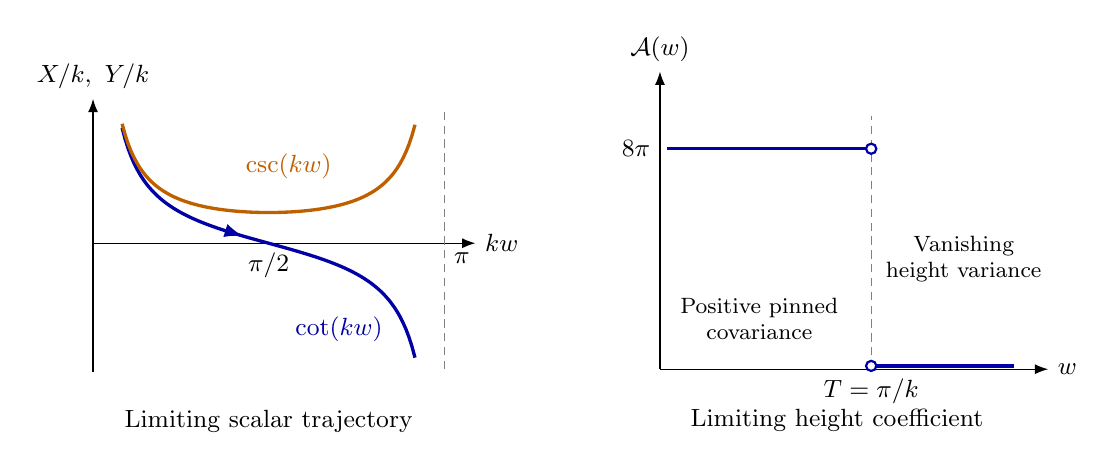
\begin{tikzpicture}[x=1cm,y=1cm,>=Latex,font=\small]
\begin{scope}[xshift=0cm,yshift=1.9cm,x=1.42cm,y=.39cm]
 \draw[->] (0,-4.2)--(0,4.7) node[above] {$X/k,\ Y/k$};
 \draw[->] (0,0)--(3.42,0) node[right] {$kw$};
 \draw[densely dashed,gray] (3.14159,-4.1)--(3.14159,4.3);
 \node[below right] at (3.14159,0) {$\pi$};
 \node[below] at (1.5708,0) {$\pi/2$};
 \draw[blue!65!black,very thick,domain=.26:2.88,samples=100]
  plot (\x,{cos(\x*180/pi)/sin(\x*180/pi)});
 \draw[orange!75!black,very thick,domain=.26:2.88,samples=100]
  plot (\x,{1/sin(\x*180/pi)});
 \node[blue!65!black,fill=white,inner sep=1pt] at (2.2,-2.8) {$\cot(kw)$};
 \node[orange!75!black,fill=white,inner sep=1pt] at (1.75,2.5) {$\csc(kw)$};
 \draw[->,blue!65!black,thick] (1.17,.43)--(1.34,.235);
 \node[align=center] at (1.57,-5.8) {Limiting scalar trajectory};
\end{scope}
\begin{scope}[xshift=7.2cm,yshift=.3cm,x=1.45cm,y=2.8cm]
 \draw[->] (0,0)--(3.4,0) node[right] {$w$};
 \draw[->] (0,0)--(0,1.35) node[above] {$\mathcal A(w)$};
 \draw[densely dashed,gray] (1.85,0)--(1.85,1.15);
 \node[below] at (1.85,0) {$T=\pi/k$};
 \draw[blue!65!black,very thick] (.06,1)--(1.85,1);
 \draw[blue!65!black,very thick] (1.85,.015)--(3.1,.015);
 \draw[blue!65!black,fill=white,thick] (1.85,1) circle[x radius=.045,y radius=.023];
 \draw[blue!65!black,fill=white,thick] (1.85,.015) circle[x radius=.045,y radius=.023];
 \node[left] at (0,1) {$8\pi$};
 \node[above,align=center,font=\footnotesize] at (.87,.09) {Positive pinned\\covariance};
 \node[above,align=center,font=\footnotesize] at (2.66,.35) {Vanishing\\height variance};
 \node[align=center] at (1.55,-.23) {Limiting height coefficient};
\end{scope}
\end{tikzpicture}
\caption{The two limits that determine the correlation length. Left: the explicit rescaled trajectory, with $k=\sqrt{3\mathcal P}$, has its outgoing pole at $w=T$. Right: the finite-scale free-height coefficient has a step at the same value. No value at the jump is asserted. Positive covariance below $T$ and circulation estimates above $T$ give the two bounds on $\delta\log_L\xi(b)$.}
\label{fig:flow-profile}
\end{figure}


\section{Finite height laws and their temperature response}\label{sec:finite}

The temperature dependence needed in the proof is already visible on a
finite graph.  We first recall the comparison inequalities for the dual
heights, and then derive a lower bound for the derivative of a height
variance.  The lower bound will later distinguish a change of temperature
from a displacement along the critical trajectory.

\subsection{Conventions and finite comparisons}

For a finite primary height graph $G=(V,E)$, orient its edges once and
write $\nabla_e h=h_{e^+}-h_{e^-}$.  The height spacing is $2\pi$ and
its edge weight is
\begin{equation}\label{eq:bessel-weight}
 p_b(k)=e^{-b}I_k(b),\qquad
 \sum_{k\in\Z}p_b(k)e^{tk}=\exp\{b(\cosh t-1)\}.
\end{equation}
In particular, $p_b$ is the distribution of the difference of two
independent Poisson variables of mean $b/2$.  Each unoriented edge
contributes one factor.  The primary Laplacian $A_G$ is normalized by
\begin{equation}\label{eq:primary-energy}
 \langle v,A_Gv\rangle=\sum_{e\in E}(\nabla_ev)^2,
\end{equation}
where all discrete pairings use counting measure.  We never replace
$A_G$ by $A_G/4$.

A free connected component of the height law is taken modulo its common
$2\pi\Z$ translations.  A representative can be pinned at one vertex
when evaluating an invariant test.  If Gaussian observations confine the
constant, all its translates are instead summed.  On a torus we use
single-valued periodic heights, hence zero winding, with the same common
translation convention.  Its height space is
$2\pi\Z^{V}/(2\pi\Z\one)$; choosing mean-zero representatives means
projecting this lattice onto the mean-zero space, rather than requiring
each projected coordinate to remain an integer multiple of $2\pi$.  Additional primary pins always have value zero
unless an affine law is specified.

Fourier expansion of the spin interaction identifies the free spin
partition function with the divergence-free integer-current sum.  Rotating
currents onto the dual edges gives the height law with exterior face
height zero.  A spin insertion at two vertices changes the divergence to
two opposite unit sources; subtracting a unit current along a path between
them gives a height law with an integral connection on the crossed dual
edges.  This is the free-boundary duality of \cite[Lemma~2.1]{X}.
It applies to the edge convention in \eqref{eq:bessel-weight}; the factors
$e^b$ cancel in every partition ratio.

We shall use the following finite comparison rules.  A centered law may
include nonnegative quadratic penalties in real linear observations,
independent Gaussian observation noises, and centered linear equalities.
An affine law has the same precision and parallel constraint space but
may have an integral edge connection, nonzero equality values, or shifted
observation centers.

\begin{lemma}[Finite comparisons]\label{lem:comparisons}
For the finite height laws just described, increasing centered precision
decreases centered covariances and real moment generating functions.
The covariance in an affine law, also after a real linear tilt, dominates
the corresponding centered covariance.  A shifted-to-centered partition
ratio is at most one and decreases when the same positive precision is
added to both laws.  The latter monotonicity also holds with a fixed real
linear statistic inserted in the exponent of the affine numerator.

Centered invariant characteristic coefficients are positive and increase
with precision.  The Hessian of their logarithm at any phase is bounded
below by its Hessian at zero.  A characteristic test on a freely translated
component is invariant when the sum of its coefficients is an integer;
a real linear test on such a component must have coefficient sum zero.
For a centered real linear test $X$,
\begin{equation}\label{eq:laplace-lower}
                    \log\E e^X\ge\tfrac12\Var(X).
\end{equation}
The same centered moment and characteristic comparisons imply that, as
$b$ increases, centered covariances and real transforms increase, whereas
centered invariant characteristic coefficients decrease.
\end{lemma}

\begin{proof}
The lattice-Gaussian inequality underlying these comparisons is due
to Regev and Stephens-Davidowitz \cite{RSD}; related extensions to
annealed integer-valued Gaussian fields appear in
\cite[Appendix~D]{AHPS}.  The statements at fixed $b$ are \cite[Lemma~2.2]{X}.  We recall the
approximation which also gives the last assertion.  Replace each primary
edge by $N$ bonds in series, with normalized lattice-Gaussian bond weight
$(b/(2N))^{k^2}$.  On compact sets of real $t$ its transform is
\[
 \frac{\sum_k(b/(2N))^{k^2}e^{tk}}
      {\sum_k(b/(2N))^{k^2}}
 =1+\frac bN(\cosh t-1)+O(N^{-2}).
\]
The full chain therefore converges to \eqref{eq:bessel-weight}, including
all fixed exponential moments.  Matching endpoints, cycle constraints,
period constraints, and the additional observations are positive
quadratic forms or limits of such forms on the enlarged lattice.  The
finite lattice-Gaussian comparison inequalities apply there.  Increasing
$b$ decreases the bond precision $2\log(2N/b)$, proving the required
monotonicities before passage to the limit.  A spanning-forest
parametrization and full-chain exponential moments dominate the sums on
each fixed primary graph.  This justifies the limit, including fixed
polynomial insertions and real tilts.  Confined constants are dominated
by their observation penalties; unconfined constants are factored out.
\end{proof}

If $X=\sum_e w_e\nabla_eh$, its \emph{reference cost} is
$\sum_e w_e^2$, minimized over flows representing the same test.  For
$X=\langle h,f\rangle$ with $\sum_xf_x=0$, the minimum is
\begin{equation}\label{eq:reference-cost}
                 G_G(f)=\langle f,A_G^+f\rangle.
\end{equation}
The analogous definition uses a grounded Laplacian when primary vertices
are pinned.

\begin{lemma}[Uniform reference bounds]\label{lem:reference-cost}
Fix a compact interval $I\subset(0,\infty)$.  In every centered finite
height law above, for $b\in I$ and each fixed $r\ge1$,
\begin{equation}\label{eq:reference-moments}
 \Var(X)\le C_I\sum_e w_e^2,\qquad
 \E|X|^r\le C_{I,r}\Bigl(\sum_e w_e^2\Bigr)^{r/2}.
\end{equation}
For every fixed $t$, the transform
$\E\exp(tX/(\sum_e w_e^2)^{1/2})$ is bounded uniformly in the graph.
More generally, if $\max_e|tw_e|\le K$, then
\begin{equation}\label{eq:bounded-flow-mgf}
                \log\E e^{tX}\le C_{I,K}t^2\sum_e w_e^2.
\end{equation}
Zero tests are interpreted separately.
\end{lemma}

\begin{proof}
Release the centered endpoint, curl, period, and observation constraints
in the full-chain construction of Lemma~\ref{lem:comparisons}.  The
comparison bounds the transform by a product of independent whole-chain
transforms.  Their limiting logarithm is
$b\sum_e(\cosh(2\pi tw_e)-1)$, which is bounded by the right side of
\eqref{eq:bounded-flow-mgf} when the arguments are bounded.  The same
bound holds uniformly in sufficiently fine subdivision.  For a flow
normalized by its Euclidean norm every coefficient has modulus at most
one.  Fixed exponential moments then give \eqref{eq:reference-moments}
and the normalized transform bound.  This is the argument of
\cite[Lemma~2.3]{X}; its constants are uniform on $I$.
\end{proof}

\subsection{Poisson insertions and a finite-volume continuity estimate}

Retain the two Poisson variables $U_e,V_e$ for every oriented edge in
\eqref{eq:bessel-weight}, and impose
$U_e-V_e=\nabla_eh/(2\pi)$.  The joint unnormalized weight is
\[
 \prod_{e\in E}e^{-b}\frac{(b/2)^{U_e+V_e}}{U_e!V_e!}
\]
with the same height constraints and observation penalties as before.
Let $N=\sum_e(U_e+V_e)$ and $M=|E|$.  For $\ell\ge0$, write
$(N)_\ell=N(N-1)\cdots(N-\ell+1)$, with $(N)_0=1$.

\begin{lemma}[Factorial insertions]\label{lem:factorial}
In a centered finite height law, including centered primary pins and
centered observation penalties,
\begin{equation}\label{eq:factorial-bound}
                         \E_b(N)_\ell\le(bM)^\ell.
\end{equation}
If the observation centers are prescribed real values, the unnormalized
factorial insertion is bounded by $(bM)^\ell$ times the corresponding
zero-observation centered sum.
\end{lemma}

\begin{proof}
Expand $(N)_\ell$ as the sum over ordered choices of $\ell$ Poisson
units, recording their edges and signs.  Removing those units leaves a
partition sum with an integral edge connection and the same primary
height variables, pins, and observation penalties.  In particular the
remaining Poisson differences obey the shifted curl and period
constraints determined by that connection.  Every removed unit
contributes $b/2$.  Lemma~\ref{lem:comparisons} bounds each shifted sum
by its centered zero-observation counterpart.  Summing the $(2M)^\ell$
choices proves the assertion.  Repeated choices of the same edge cause
no difficulty: falling factorials are exactly the factors canceled by
removing several units from its Poisson factorial.
\end{proof}

For a fixed finite graph with observations $\eta$, let $\mu_b^\eta$
denote its unnormalized joint weight, including the Poisson variables,
and let $Z_b^0$ denote its centered zero-observation mass.  The graph may
have centered hard pins; these are included in both objects.

\begin{lemma}[Finite-volume parameter continuity]\label{lem:finite-perturbation}
Fix $b_0>0$ and a compact set $K$ of complex observation vectors on a
fixed finite list of observation shapes.  There are constants $c,C>0$
such that, for $\eta\in K$ and $|b-b_0|M\le c$,
\begin{equation}\label{eq:finite-tv}
 \frac{\|\mu_b^\eta-\mu_{b_0}^\eta\|_{\rm TV}}{Z_{b_0}^0}
                   \le C|b-b_0|M.
\end{equation}
Here total variation for complex weights means the sum of their absolute
values.  The constants can be uniform over any prescribed finite family
of graph topologies and observation shapes.  In particular, each
centered normalizer is nonzero on a disk of radius $c/M$ about $b_0$.
\end{lemma}

\begin{proof}
The parameter likelihood in the augmented variables is exactly
\begin{equation}\label{eq:poisson-likelihood}
       \exp\{-(b-b_0)M\}(b/b_0)^N.
\end{equation}
Expand the second factor in falling factorials.  For real observations,
Lemma~\ref{lem:factorial} bounds the absolute sum of its positive-order
terms, divided by $Z_{b_0}^0$, by
\[
 \sum_{\ell\ge1}\frac{|b-b_0|^\ell}{\ell!b_0^\ell}(b_0M)^\ell
                  =e^{|b-b_0|M}-1.
\]
The scalar exponential in \eqref{eq:poisson-likelihood} has the same
bound.  For $\eta=\eta_1+i\eta_2$, the absolute observation penalty is
its real-$\eta_1$ penalty times $e^{\|\eta_2\|^2/2}$, uniformly bounded
on $K$.  This proves \eqref{eq:finite-tv}.  At zero observation it gives
$|Z_b^0/Z_{b_0}^0-1|<1/2$ after decreasing $c$, hence nonvanishing.
All sums are analytic on compact parameter sets by the same expansion.
\end{proof}

\subsection{A strict response bound}

The upper bound in Lemma~\ref{lem:reference-cost} alone does not imply
that changing $b$ moves the long-scale height coefficient.  The following
inequality supplies the needed strict response using only finite graphs.

\begin{lemma}[Temperature response]\label{lem:response}
Let $G$ be a finite connected graph with the centered Bessel height law,
and let $f\ne0$ have coefficient sum zero.  Set
$X=\langle h,f\rangle$ and $G(f)=\langle f,A_G^+f\rangle$.
For $b$ in a compact interval $I\subset(0,\infty)$,
\begin{equation}\label{eq:temperature-response}
 \frac{\Var_b(X)^2}{4\pi^2b^2G(f)}
       \le \partial_b\Var_b(X)
       \le C_I|E|G(f).
\end{equation}
In particular, these inequalities hold on every zero-winding periodic
torus, with constants independent of its size.
\end{lemma}

\begin{proof}
Let $C_b$ be the covariance operator on mean-zero tests.  For each
oriented edge $e$, removing one positive Poisson unit gives the shifted
height weight
\[
 \prod_{d\in E}p_b\bigl(\nabla_dh/(2\pi)-\one_{\{d=e\}}\bigr).
\]
Let $r_e$ be its partition sum divided by the centered sum, and $v_e$
its mean of $X$.  Reversing $h$ identifies the negative-removal law with
its reflection, so its partition ratio is $r_e$ and its mean is $-v_e$.
By Lemma~\ref{lem:comparisons}, $0<r_e\le1$ and each shifted variance
is at least $\Var_b(X)$.

Differentiating the normalized augmented law inserts the score $N/b$;
the deterministic term $-|E|$ cancels.  Since the centered mean of $X$
is zero,
\[
 \partial_b\Var_b(X)=b^{-1}\Cov_b(X^2,N).
\]
Removing a positive or negative unit separately now gives the exact
identity
\begin{equation}\label{eq:response-insertions}
 \partial_b\Var_b(X)
   =\sum_{e\in E}r_e\bigl(\Var_{e,+}(X)-\Var_b(X)+v_e^2\bigr)
   \ge\sum_{e\in E}r_ev_e^2.
\end{equation}
The same removal with the insertion $X$ gives
\[
 \E_b[(U_e-V_e)X]=br_ev_e.
\]
As $\nabla_eh=2\pi(U_e-V_e)$, this is
\begin{equation}\label{eq:response-gradient}
                    \nabla_e(C_bf)=2\pi br_ev_e.
\end{equation}
Discrete integration by parts and Cauchy--Schwarz yield
\[
 \begin{split}
 \Var_b(X)^2
 &=\langle\nabla A_G^+f,\nabla C_bf\rangle^2\\
 &\le G(f)\sum_e|\nabla_eC_bf|^2
 \le4\pi^2b^2G(f)\sum_er_ev_e^2.
 \end{split}
\]
Together with \eqref{eq:response-insertions}, this proves the lower
bound.  For the upper bound, Lemma~\ref{lem:factorial} gives
$\E N^2\le(bM)^2+bM$, while
Lemma~\ref{lem:reference-cost} gives $\E X^4\le C_IG(f)^2$.
Cauchy--Schwarz in the score identity proves
$|\partial_b\Var_b(X)|\le C_IMG(f)$, since $M\ge1$ and $b\in I$.
The finite-volume analyticity established above justifies every
differentiation.  No bound on the inverse precision of a subdivided
Gaussian chain is used.
\end{proof}

\section{Analytic entry and the activity coordinates}\label{sec:entry}

We now connect the finite height laws to the small-activity map of
\cite{F}.  The map itself acts on analytic functions and is independent
of the temperature of the physical input.  The point requiring a new
argument is initialization: the critical construction must remain small
on a parameter disk large enough to differentiate with respect to $b$.
We prove this on a disk of radius proportional to $s^{-2}$, where $s$ is
the observation-cell side.  All constants depending on fixed geometric
parameters are chosen before $s$ tends to infinity.

\subsection{The reference field and the initialization norm}

The critical free-height coefficient is $a=8\pi$ by
\cite[Section~6]{X}.  Fix $\alpha=\sqrt a$ and $\omega=2\pi/\alpha$.
The reference field has covariance $A^+$, so that $\alpha$ times the
reference field has height covariance $aA^+$.  We keep this reference,
including $\alpha$, fixed when $b$ varies.

Partition the primary graph into whole square cells of side $s$, let
$B_s$ average over each cell, and introduce the observations
\begin{equation}\label{eq:observations}
                         \eta=B_sh+e,
\end{equation}
where the components of $e$ are independent standard Gaussians.  On a
retained graph $G$, let $Z_{G,b}(\eta)$ be the height partition sum with
penalty $\exp(-\|B_sh-\eta\|^2/2)$, and define the fixed reference energy
\begin{equation}\label{eq:observation-energy}
 E_G(\eta)=\min_{v\in\R^{V(G)}}
       \{a^{-1}\|\nabla v\|_G^2+\|B_sv-\eta\|^2\}.
\end{equation}
Each component constant is free in this minimization.  For a retained
cell face $f=(Q,Q')$, put $w_f=\eta_{Q'}-\eta_Q$ and use the entire
cutoff
\begin{equation}\label{eq:entry-cutoff}
 \chi_s(z)=
 \frac{\int_{-s}^s e^{-(z-t)^2/2}\,dt}{\int_{-s}^se^{-t^2/2}\,dt},
 \qquad
 \widehat Z_{G,b}(\eta)=Z_{G,b}(\eta)\prod_f\chi_s(w_f).
\end{equation}
A deleted face loses both its primary bonds and its cutoff factor.

Here are the reference split and norm used in \cite{F}.  For an integer
$u\ge1$, set
\[
 P_u(\cos t)=\left(\frac{\sin(ut/2)}{u\sin(t/2)}\right)^{64},
 \qquad \mathsf P_u=P_u(1-A/64),
\]
with removable values understood, and put
\begin{equation}\label{eq:reference-split}
 C_{<u}=A^{-1}(I-\mathsf P_u),\qquad
 \Gamma_u=A^{-1}(\mathsf P_u-\mathsf P_{Lu}),\qquad
 C_{\ge u}=A^+\mathsf P_u.
\end{equation}
The first two quotients have polynomial continuations at the constant
mode.  They have finite range and are positive.  Their constant modes
can be integrated because the final common mean is uniform modulo
$\omega$.

At side $u$, a polymer is a finite set $X$ of $u$-blocks connected for
the fixed adjacency of \cite{F}.  Its occupied support is the union of
those blocks.  The field dependence of $K(X,\phi)$ is confined to this
support together with the prescribed microscopic collar of
\cite[Proposition~4.1]{F}, whose width is at most a fixed sufficiently
small fraction of $u$.  This dependence region is distinct from the
larger norm padding $D_u(X)$, which is enlarged to whole observation
cells and contains all fixed difference stencils.

We use the bulk symmetry class of \cite[Theorem~4.6(i)]{F}.
Its activities are analytic in the field and satisfy
\begin{equation}\label{eq:bulk-activity-symmetries}
 K(X,-\phi)=K(X,\phi),\qquad
 K(X,\phi+\omega\one)=K(X,\phi),\qquad
 K(gX,g\phi)=K(X,\phi),
\end{equation}
where $g$ is a compatible block translation or square-lattice rotation
or reflection and $(g\phi)(v)=\phi(g^{-1}v)$.  Compatibility means
that $g$ preserves the chosen block and observation grids.  On a torus
we impose the corresponding periodic support and covariance rules.
These identities are complex-linear conditions on the activity;
reality on real fields is a separate property.  The point norm is
\begin{equation}\label{eq:entry-point-norm}
 \begin{split}
 \|f\|_{u,D}&=\max_{v\in D}\{|f(v)|,u|\nabla f(v)|,
                                           u^2|\nabla^2f(v)|\},\\
 |K(X)|_{u,\phi}
 &=\sum_{r\ge0}\frac{h_0^r}{r!}
   \sup_{\|f_i\|_{u,D_u(X)}\le1}
       |D^rK(X,\phi)[f_1,\ldots,f_r]|.
 \end{split}
\end{equation}
Let $\mathscr W_u^\kappa(X,\phi)$ be the ordinary exponential regulator
specified in \cite[Section~4.2, Equations~(41)--(43)]{F}; it controls the bulk gradient energy,
its boundary trace, and scaled second differences.  The additional
observation regulator is given explicitly by
\begin{equation}\label{eq:entry-observation-regulator}
 V_u(X,\phi)=\frac12\sup_{\zeta,e}
 \left\{h_*E_{D_u(X)}\bigl(B_s\alpha(\phi+\zeta)+e\bigr)
       -p_1^{-1}(\|\zeta\|_{C_{<u}}^2+\|e\|^2)\right\}.
\end{equation}
The Cameron norm is taken on the covariance support.  With a fixed block
weight $A_w>1$, the activity norm is
\begin{equation}\label{eq:entry-activity-norm}
 \|K\|_{u,s}=\sup_{X,\phi}
 A_w^{|X|}\frac{|K(X)|_{u,\phi}}
                  {\mathscr W_u^\kappa(X,\phi)e^{V_u(X,\phi)}}.
\end{equation}
Write $\mathscr A^{\mathrm{bulk}}_{u,s}$ for the complex space of
activity families satisfying the support and symmetry conditions above
and having finite norm \eqref{eq:entry-activity-norm}.  Every activity
ball and activity variation below is taken in this space or its
compatible-torus counterpart.  The ordinary regulator is kept exactly
as in the cited construction; its shell averaging and translation estimates, together with the
explicit observation regulator, are part of the imported local-map
bounds below.  Norms with different observation sides $s$ need not be
identified.

The cutoff gives a strict large-field reserve.  Indeed, adjacent-cell
averages have a primary flow representation with coefficient bound
$C/s$ and squared cost $C$.  Applying
\eqref{eq:bounded-flow-mgf} with tilts of size at most a fixed multiple
of $s$, then using the Gaussian tails of $\chi_s$, gives uniformly for
$b$ in a compact neighborhood of $\bc$
\begin{equation}\label{eq:entry-large-field}
 e^{E_G(\eta)/2}\frac{\widehat Z_{G,b}(\eta)}{Z_{G,b}(0)}
             \le e^{(1-c_*)E_G(\eta)/2},\qquad \eta\in\R^{\mathcal Q(G)},
\end{equation}
for some fixed $c_*>0$ on every retained topology used in the
construction.  More explicitly, transporting each site straight to its
translate in a neighboring cell gives flows $\Phi_f$ with
\[
 \max_e\left|\sum_ft_f\Phi_f(e)\right|\le Cs^{-1}\max_f|t_f|,
 \qquad \sum_e\left|\sum_ft_f\Phi_f(e)\right|^2\le C\sum_ft_f^2.
\]
The tilted affine comparison applies also at prescribed observations;
releasing the height and noise equalities gives a bound
$\exp(C\sum_ft_f^2)$.  Choose
$t_f$ proportional to $\operatorname{sgn}(w_f)\min(|w_f|,s)$.
For $|w_f|>s$ the cutoff supplies the remaining quadratic decay.
Finally $E_G(\eta)\le C\sum_fw_f^2$, by cell interpolation.
These are the steps in \cite[Lemma~4.4 and Equation~(57)]{F}; the only physical transform
used there is $\exp\{b(\cosh(2\pi t)-1)\}$, whose constants are uniform
on the chosen $b$ interval.

Choose fixed parameters with strict inequalities
\begin{equation}\label{eq:entry-reserves}
        1-c_*<h_1<h_*<1/p_2,\qquad 1<p_1<p_2.
\end{equation}
There is also slack in the exponent of $\mathscr W$.  Choose the fixed
analytic radius, field-strip widths, and a sufficiently large dyadic
$L$ as in \cite{F}; then choose the activity weights and the small
map domain.  Fix its coloring period $q$, choose a sufficiently large
dyadic $R_0$, and set $P_0=R_0^5$.  An admissible observation side
satisfies
\begin{equation}\label{eq:entry-side}
                         qR_0s=L^{j_0}.
\end{equation}
The index $j_0$ is absolute, rather than reset to zero at entry.
The choice of $R_0$ remains subject to any further fixed small-tube
requirements made below; all such choices precede the limits in $s$
and $b$.

\subsection{A parameter disk for initialization}

We use the finite initialization of \cite{F} with no magnetic or
compulsory component.  On a compatible finite torus it represents the
cutoff law exactly, up to a field-independent scalar, after averaging
$e$ and the Gaussian field with covariance $C_{<L^{j_0}}$.  The
corresponding plane activities are defined by the same local formulas.
For clarity, the partition functional of an activity is
\[
 \mathcal Z_u(K;\phi)=\sum_{V\subset\mathcal B_u}
                         \prod_{X\in\operatorname{Comp}(V)}K(X,\phi),
\]
where components use the fixed block adjacency and the empty product
is one.  The representation identifies the averaged cutoff interaction
with a scalar times $\mathcal Z_{L^{j_0}}$.

\begin{proposition}[Analytic initialization]\label{prop:entry}
For every sufficiently small $\rho>0$, the fixed choices above can be
made so that there exist $c_{R_0}>0$ and $s_0<\infty$ with the following
property.  For every admissible $s\ge s_0$, the ordinary plane and
compatible-torus entry activities $K_s(b)$ are Banach analytic on
\begin{equation}\label{eq:entry-parameter-disk}
                         |b-\bc|<c_{R_0}s^{-2},
\end{equation}
and take values in $\mathscr A^{\mathrm{bulk}}_{L^{j_0},s}$ or its
compatible-torus counterpart, with norm at most $\rho$.
They are real on real fields when $b$ is real.  Their support,
symmetry, and local copying identities agree with those at criticality
throughout the complex parameter disk.
For real parameters in this disk the cutoff partition representation
is exact.  On a smaller concentric disk, for each fixed $r\ge1$,
\begin{equation}\label{eq:entry-cauchy}
                \|\partial_b^rK_s(b)\|_{L^{j_0},s}
                              \le C_{R_0,r}s^{2r}.
\end{equation}
\end{proposition}

\begin{proof}
We first describe the parts of the finite expansion whose estimates
have to be extended.  The geometry and algebra are those of
\cite[Sections~4.6--4.7, Theorem~4.6]{F}; only their physical weights change with $b$.
The observation cells are partitioned into tiles of side comparable to
$R_0$.  A finite colored sequence of isolation events deletes the
remaining bonds between tiles.  At an event with open patch $o_i$ and
cut patch $c_i$, its proxy is
\begin{equation}\label{eq:entry-proxy}
 \mathcal B_i(b,\eta)=C_i(b)
                  e^{-(E_{o_i}(\eta)-E_{c_i}(\eta))/2},\qquad
 C_i(b)=\frac{Z_{o_i,b}(0)}{Z_{c_i,b}(0)}.
\end{equation}
One writes the original factor as its proxied cut factor plus their
difference.  Selecting the difference marks that event.  Later events
within its fixed neighborhood are skipped.  After the finite sequence,
undeleted intertile bonds lie in the union of the marked neighborhoods.
We call each connected part of this union a halo.  Outside the halos,
an isolated tile contributes either one or its normalized factor minus
one.  The latter choice is a selected tile.

The remaining Gaussian mismatch is expanded in links
$e^{b_\ell w_fw_{f'}}-1$, with
\begin{equation}\label{eq:entry-links}
                         |b_\ell|\le Ce^{-c(R_0+d_\ell)}.
\end{equation}
Here $d_\ell$ records the entire tagged path length, including winding
on a torus.  A link covers at most $C(1+d_\ell/R_0)$ entry blocks.
An individual pattern $\pi$ consists of marked events, selected tiles,
and links, with their complete occupied cover $X(\pi)$.  Write $l(\pi)$
for the number of marks and selected tiles.  Each of these physical
items uses at most $C_{R_0}$ observation cells and $C_{R_0}s^2$ primary
edges.  Link-only cells carry no physical height factor.  All identical
factors off the affected halos cancel before the pattern is defined.
Its denominator is a product of the affected local scalars $C_i(b)$
and isolated-tile normalizers $Z_{Q,b}(0)$.  In particular, a centered
partition function of an arbitrarily large halo is not a denominator
of a defining pattern.

We keep every Gaussian energy in \eqref{eq:entry-proxy} fixed.  Thus the
finite algebra, the link coefficients, the occupied covers, and the
copying identities remain valid with the actual parameter in every
physical factor and scalar normalizer.  It remains to bound and sum the
resulting patterns.

\paragraph{Real parameters.}
In the critical proof a positive expansion of each marked difference
introduces a conditional factor
\begin{equation}\label{eq:entry-mark-fraction}
 d_i(\eta,\gamma)=
 \frac{|K_{o_i}(\eta,\gamma)-\mathcal B_i(\eta)K_{c_i}(\eta,\gamma)|}
      {K_{o_i}(\eta,\gamma)+\mathcal B_i(\eta)K_{c_i}(\eta,\gamma)}
                         \le1.
\end{equation}
The kernels prescribe the primary guard values $\gamma$ surrounding
the event.  Exterior factors common to the two choices cancel in this
ratio.  The halo is then cut into boxes of side $P_0$ in cell units.
Only guards whose testing neighborhoods lie inside a box are retained.
Affine comparison bounds the joint observation and guard densities
before and after cutting.  The resulting centered zero-guard ratio is
bounded by a product of local separated-pin comparisons.  Gaussian
shape errors have small face-square coefficients.  This is precisely
the positive-topology and seam accounting in
\cite[Equations~(71)--(74)]{F}.

After $R_0,P_0$, the field strips, and the large-field threshold are
fixed, the compact-data part of this argument concerns finitely many
box topologies.  Each has at most $C_{R_0}s^2$ primary edges.  A box is
called good when the sum of squared differences on its underlying cell
faces is below that fixed threshold.  Period recentering places its
observations in a fixed compact set.  The critical inputs in
\cite[Proposition~2.3 and Equations~(75)--(80)]{F} give on these compact sets: bounds on normalized positive
box factors, separated-pin restoration bounds, and a small fixed list
of moments of the fractions \eqref{eq:entry-mark-fraction}.  The list
includes all H\"older orders required by the finite number of marks
which a $P_0$-box can contain.  All inequalities are used with strict
slack.

Lemma~\ref{lem:finite-perturbation}, applied to these finite graphs,
preserves the required tolerances when
$|b-\bc|\le c_{R_0}s^{-2}$.  For centered pin interactions one applies
the lemma to each pinned sum itself, so that a small absolute change
in an unpinned normalization is never used as a relative estimate for
a rare pin event.  On real compact observation sets,
\[
 Z_{G,b}(\eta)/Z_{G,b}(0)
 =e^{-\|\eta\|^2/2}\E_{G,b,0}e^{\langle\eta,B_sh\rangle}
                       \ge e^{-\|\eta\|^2/2},
\]
which converts normalized total-variation estimates to the needed
relative estimates.

The conditional fractions require some care because the guards have
an increasing number of primary vertices.  For one retained event,
use the two complete adjacent positive box topologies and let
$A_b(\gamma),B_b(\gamma)$ be their joint weights, incorporating the
proxy and cutoff scalars.  Their total masses are comparable, uniformly
on the fixed compact set: at zero observation this follows from the
open and zero-guard brackets and the bounded separated-pin interaction;
for other compact observations it follows from the preceding lower
bound and the upper affine comparison.  Lemma~\ref{lem:finite-perturbation}
controls both arrays in $\ell^1$, in units of either total mass.
For nonnegative $A,B,A',B'$,
\[
 (A+B)\left|
 \frac{|A-B|}{A+B}-\frac{|A'-B'|}{A'+B'}\right|
 \le2(|A-A'|+|B-B'|),
\]
with the continuous convention at a zero denominator.  The same
estimate for the $r$th power has an additional factor at most $r$.
Consequently every required fixed moment of $d_i$ changes by a quantity
tending to zero with $c_{R_0}$.  No estimate uniform in individual guard
values is needed.  The compact imaginary-observation estimates after
pinning strips are preserved by the complex version of
Lemma~\ref{lem:finite-perturbation}.

The remaining inputs are uniform finite comparisons and
\eqref{eq:entry-large-field}.  They control the boxes outside the
compact set with the same reserves.  The deterministic Gaussian
localization, link estimates, and counting do not involve $b$.
Repeating the real and complex-field interpolation of
\cite[Lemma~4.7, Equations~(85)--(89)]{F} therefore gives, on fixed field disks with radius
larger than the polarization radius needed in
\eqref{eq:entry-point-norm},
\begin{equation}\label{eq:entry-real-pattern}
 |F_\pi(b;\phi+zf)|
 \le C^{l(\pi)}e^{-cR_0l(\pi)}
       \prod_{\ell\in\pi}Ce^{-c(R_0+d_\ell)}
       \mathscr W_{L^{j_0}}^\kappa(X,\phi)e^{V_{L^{j_0}}(X,\phi)}.
\end{equation}
Here $b$ is real in the parameter interval, $\phi$ is real,
$\|f\|_{L^{j_0},D}\le1$, and $|z|$ is in that fixed disk.
The constants in the exponential gains may have decreased.

We have extended the small real-parameter bound.  To obtain parameter
Cauchy estimates we next need an analytic bound on a complex disk; this
bound need not retain the small factor attached to each physical item.

\paragraph{A complex-parameter majorant in the same norm.}
Let $r_s=c_{R_0}s^{-2}$ and $b_+=\bc+r_s$.  For $|b-\bc|\le r_s$ we
have $|b|\le b_+$.  On a positive physical branch containing $N_\pi$
retained primary edges, absolute augmented Poisson weights satisfy
\begin{equation}\label{eq:complex-poisson-majorant}
 \left|\prod_e e^{-b}\frac{(b/2)^{U_e+V_e}}{U_e!V_e!}\right|
 \le e^{(b_+-\Re b)N_\pi}
       \prod_e e^{-b_+}\frac{(b_+/2)^{U_e+V_e}}{U_e!V_e!}.
\end{equation}
The physical support count gives $N_\pi\le C_{R_0}l(\pi)s^2$.
Each local scalar normalizer is nonzero in this disk by
Lemma~\ref{lem:finite-perturbation}; its value and its inverse, relative
to the corresponding value at $b_+$, cost at most a fixed factor.
There are $O(l(\pi))$ affected scalars.  Expand each marked difference
into its two terms and compare their unnormalized physical numerators
by \eqref{eq:complex-poisson-majorant}, and their local scalar factors
separately.  The result is bounded by $e^{C_{R_0}l(\pi)}$ times the
corresponding positive pattern at $b_+$.  At this point one may apply
the real positive-topology estimate at $b_+$.  This ordering uses no
complex partition function of a large connected halo.

For a field displacement $zf$ in the fixed field disk, every imaginary
observation coordinate is bounded.  The absolute observation penalty
costs $e^{\|\Im\eta\|^2/2}$ on each physical factor.  There are at
most $C_{R_0}l(\pi)$ such coordinates, including the local proxies.
The real quadratic forms satisfy
\[
                 \Re E_G(\eta_1+i\eta_2)=E_G(\eta_1)-E_G(\eta_2).
\]
Their imaginary contributions therefore also cost at most
$e^{C_{R_0}l(\pi)}$.  For the real parts keep the Gaussian shapes
combined into the reference mismatch before estimating them.  It
consists of the energy of the actual positive physical topology and
the small localized proxy and link errors.  Thus overlapping proxy
patches do not create overlapping broad-energy charges.

More explicitly, after dropping the fractions $d_i$, the large-field
bound may be used on every actual halo piece and every separate
selected-tile factor.  Its broad quadratic cost is
\begin{equation}\label{eq:complex-broad-charge}
                   \frac{1-c_*}{2}\sum_B E_B(\eta_1).
\end{equation}
The actual graphs $B$ are disjoint: selected tiles lie outside the halo
graph and are mutually isolated.  Restricting a trial field for the
open energy on $D=D_{L^{j_0}}(X)$ to each of them gives
$\sum_BE_B\le E_D$.  The remaining proxy, seam, and link costs have
small coefficients on underlying face differences with bounded
per-face sum.  The cell flow estimate bounds each such face square
by the energy of its two underlying cells.  Taking $R_0$ large leaves
these costs inside the strict gap $h_1-(1-c_*)$.  Hence the complete
positive real-variable quadratic form $q_\pi$ obeys
\begin{equation}\label{eq:complex-form-domination}
                           q_\pi(\eta_1)\le\tfrac12h_1E_D(\eta_1).
\end{equation}
This is the form domination of \cite[Equation~(82)]{F}, with all physical boxes
now charged broadly.  Its coefficient and its ambient open energy are
unchanged.

To see that the determinant is still harmless, write the averaging
variables as a standard Gaussian vector $\zeta$ and
$\eta_1=d+\mathsf S\zeta$.  Set
$M_\pi=\nabla_\zeta^2[p_1q_\pi(d+\mathsf S\zeta)]$.
The covariance contraction for the observation energy and
\eqref{eq:complex-form-domination} give
$0\le M_\pi\le p_1h_1I<I$.  Gaussian completion is exactly
\begin{equation}\label{eq:complex-entry-completion}
 \bigl(\E e^{p_1q_\pi(d+\mathsf S\zeta)}\bigr)^{1/p_1}
 =\det(I-M_\pi)^{-1/(2p_1)}
  \exp\sup_\zeta\left\{q_\pi(d+\mathsf S\zeta)
                                  -\frac{\|\zeta\|^2}{2p_1}\right\}.
\end{equation}
The supremum is bounded by the same $V_{L^{j_0}}(X,\phi)$ in
\eqref{eq:entry-observation-regulator}.  A broad energy has rank at most
its number of observation coordinates, as in
\cite[Equations~(83)--(84)]{F}.  There are at most
$C_{R_0}l(\pi)$ physical coordinates; proxy errors keep their small
coefficients.  Link-only cells enter through the reserved link cost,
not a broad rank.  The trace bound is consequently
\begin{equation}\label{eq:complex-entry-trace}
 \operatorname{tr}M_\pi\le C_{R_0}l(\pi)
       +C\sum_{\ell\in\pi}e^{-c(R_0+d_\ell)}
                                      \operatorname{poly}(d_\ell).
\end{equation}
A face contrast has uniformly bounded reference variance by the cell
flow bound, which proves the second term, even for arbitrarily long
links.  Since $\|M_\pi\|$ is bounded away from one,
$-\log\det(I-M_\pi)\le C\operatorname{tr}M_\pi$.
H\"older's inequality handles the ordinary regulator with its fixed
exponent reserve.  Translation by the bounded real part of $zf$ costs
$e^{C|X|}$.  Such a factor can be absorbed by weakening the gains of
\eqref{eq:entry-links}, because each link occupies only
$O(1+d_\ell/R_0)$ blocks.  The exponential gain per physical item is
not retained in this coarse estimate.

We have obtained, on the same field disks and in the same regulators,
\begin{equation}\label{eq:entry-complex-pattern}
 |F_\pi(b;\phi+zf)|
 \le e^{C_{R_0}l(\pi)}
       \prod_{\ell\in\pi}Ce^{-c(R_0+d_\ell)}
       \mathscr W_{L^{j_0}}^\kappa(X,\phi)e^{V_{L^{j_0}}(X,\phi)}.
\end{equation}
The domination also proves analyticity of each pattern after Gaussian
averaging.  All scalar denominators are local and nonzero, and the
integrals converge absolutely on compact parameter and field disks.

\paragraph{Recovering smallness in the parameter disk.}
For fixed $\pi,\phi,z,f$, apply the two-constants theorem to the upper
and lower half-disks $|b-\bc|<r_s$.  On the real diameter use
\eqref{eq:entry-real-pattern}; on the semicircle use
\eqref{eq:entry-complex-pattern}.  If $|b-\bc|\le\vartheta r_s$, the
harmonic measure of the semicircle is at most $\omega(\vartheta)$,
where $\omega(\vartheta)\to0$ as $\vartheta\downarrow0$.  The
regulator and a common weakened link product are independent of $b$
and can be divided out.  The resulting item factor is at most
\[
 \exp\{[-(1-\omega(\vartheta))cR_0
                         +\omega(\vartheta)C_{R_0}+C]l(\pi)\}.
\]
Choose $\vartheta>0$, depending only on $R_0$, so that its exponent is
at most $-cR_0l(\pi)/2$, after enlarging $R_0$ if needed.  Thus the
small pattern bound holds on the reduced complex parameter disk.
For patterns containing only links, both boundary estimates already
have the common link gains.

The fixed field disk has radius exceeding the polarization radius in
\eqref{eq:entry-point-norm}.  Cauchy's formula and polarization
therefore sum all field derivatives with that norm.  Connected
summation over the complete occupied covers, with the gains just
proved, is the same absolutely convergent sum as in
\cite[Theorem~4.6]{F}.  Its norm is at most $Ce^{-cR_0}$, uniformly in
$s$, the absolute entry index, and compatible volume.  The same bound
on compact parameter disks makes the sum Banach analytic.  Absorb
$\vartheta$ into $c_{R_0}$ and choose $R_0$ to reach the prescribed
$\rho$.  Parameter Cauchy estimates give \eqref{eq:entry-cauchy}.
The occupied covers retain every field dependency, as in the critical
construction.  The covariant placement and color rules, reference
Gaussian averaging, and field-negation identities are unchanged when
only the physical weights and centered scalar normalizers depend on
$b$.  Thus \eqref{eq:bulk-activity-symmetries} and the prescribed collar
rules hold throughout the parameter disk.  The exact finite algebra
and real positive normalizers give the partition representation for
real $b$, and the same local formulas give the copying identities.
\end{proof}

\subsection{The map at fixed reference}

The initialization puts the entire activity into the remainder.  At a
later side $L^j$, separate two singleton functions on each regular block:
\[
 e_B^0(\phi)=\frac12\sum_{v\in B}\sum_{e=\pm e_1,\pm e_2}
                                      |\nabla_e\phi(v)|^2,
 \qquad
 c_B^\alpha(\phi)=L^{-2j}\sum_{v\in B}\cos(\alpha\phi_v).
\]
Their coefficients are denoted by $t_j/2$ and $z_j$; the remaining
activity is $\mathcal R_j$.  Block covariance makes these coefficients
independent of the block.  Field negation excludes the sine singleton,
and square symmetry makes the retained neutral gradient quadratic
isotropic.  These are the two scalar directions in the bulk weak map
of \cite[Section~5.1]{F}.  The exact map integrates the shell
$\Gamma_{L^j}$, removes designated field-independent factors, and
reexpresses the result in the same subset partition algebra.  The
following interface collects the activity estimates used in the rest
of the paper.

\begin{proposition}[Activity map]\label{prop:map}
For all sufficiently large absolute indices $j$, the map on
$(t,z,\mathcal R)\in\mathbb C^2\times
\mathscr A^{\mathrm{bulk}}_{L^j,s}$, with the occupied-support and
designated-localization conventions of \cite[Proposition~4.1]{F},
preserves the bulk symmetry class and is analytic on a fixed ball
$|t|+|z|+\|\mathcal R\|_{L^j,s}<\rho_{\mathrm{map}}$.
Its linear part is
\begin{equation}\label{eq:map-triangular}
 (t,z,\mathcal R)\longmapsto
   (t+P_j^t\mathcal R,\lambda_jz+P_j^z\mathcal R,
                                                \mathsf C_j\mathcal R),
 \quad \|\mathsf C_j\|\le\theta_0<1,
 \quad \lambda_j=1+O(e^{-cj}),
\end{equation}
with uniformly bounded rows $P_j^t,P_j^z$.  The nonlinear part and its
Taylor derivatives have quadratic bounds with uniform constants.

There are analytic normal coordinates $(u,Z,Q)$, uniform in the entry
side, such that the pure Gaussian curve is $(u,0,0)$ and the map fixes
$u$ on that curve.  With $b_*=2\log L$ and a constant $H>0$, define
\begin{equation}\label{eq:balanced-coordinates}
                  x=b_*u,\qquad y=\sqrt{b_*H}\,Z,\qquad W=(x,y).
\end{equation}
The coordinate changes obey
\begin{equation}\label{eq:coordinate-comparison}
 t=u+O(u^2+\|Q\|),\qquad
 z=(1+O(e^{-cj}))Z+O(u^2+\|Q\|),\qquad
 \mathcal R=O(u^2)+Q,
\end{equation}
with the differentiated analytic bounds of these orders.  In a fixed
small tube,
\begin{equation}\label{eq:normal-map}
 \begin{split}
 W_+&=W+(-y^2,-xy)+\mathcal E_j(W,Q),\\
 |\mathcal E_j(W,Q)|
 &\le C\{j^{-2}|W|^2+|W|^3+(|W|+\|Q\|)\|Q\|\},\\
 \|Q_+\|&\le\theta\|Q\|+C|W|^2,\qquad \theta<1.
 \end{split}
\end{equation}
The error is an analytic function with the corresponding Taylor
bounds on all fixed derivatives.

On a separately initialized compatible torus with a fixed range buffer,
the two singleton coefficients copy the plane coefficients through its
stop.  The torus remainder has its own contraction and analytic
quadratic bound.  Its derivative at zero has no singleton forcing.
All constants are uniform in the stop, the entry side, and their
associated norms.
\end{proposition}

\begin{proof}
The exact activity map and its uniform norm bounds are
\cite[Proposition~4.1]{F}; the triangular form is
\cite[Equation~(93)]{F}.  We recall the coordinate construction to
specify the derivative bounds being used.  Put
$\ell_j=\prod_{h\ge j}\lambda_h=1+O(e^{-cj})$ and
$\mathsf C_{h:j}=\mathsf C_{h-1}\cdots\mathsf C_j$.  The balanced
linear coordinates are
\[
 T=t+\sum_{h\ge j}P_h^t\mathsf C_{h:j}\mathcal R,
 \qquad
 Z=\ell_jz+\sum_{h\ge j}\ell_{h+1}P_h^z\mathsf C_{h:j}\mathcal R.
\]
The series converge geometrically.  At the chosen entry, initialize an
exact Gaussian interaction $\exp(d\sum_Be_B^0/2)$ and iterate the
same map.  Its balanced gradient is $T_j^g(d)=d+O(d^2)$ and its
remainder is $\mathcal R_j^g(d)=O(d^2)$, uniformly on a common complex
disk.  Define $u=(T_j^g)^{-1}(T)$ and
$Q=\mathcal R-\mathcal R_j^g(u)$, as in
\cite[Equations~(95), (99), and (101)]{F}.  This gives
\eqref{eq:coordinate-comparison}; in particular its linear remainder
rows are bounded, while derivatives of its quadratic scalar terms are
$O(|u|)$.

The parity estimates of \cite[Lemma~5.2]{F} give leading scalar terms
$-H_jZ^2$ and $-b_juZ$, with no nonconstant term on the Gaussian curve.
Their remainders have the differentiated orders used in
\eqref{eq:normal-map}.  Moreover
\cite[Lemma~5.3]{F} gives
$|H_j-H|+|b_j-b_*|\le C(1+j)^{-2}$.
Rescaling by \eqref{eq:balanced-coordinates} yields the displayed
map.  Terms with a small coefficient multiplying $Q$ are absorbed into
a slightly larger contraction constant.  The copying assertion and the
separate torus contraction are part of the same local-map statement;
no equality between plane and torus remainders is required.
\end{proof}

The triangular contraction also has a useful elementary consequence.
In equivalent scalar and remainder norms, the derivative of the full
map on a sufficiently small tube has norm at most $1+\gamma$, for any
prescribed $\gamma>0$.  To see this, first use the balanced coordinates,
whose scalar linear rows contain no remainder, and choose a product
norm with the fixed remainder contraction.  At zero the operator norm
is at most one.  Uniform analytic derivative bounds then give the
claim on a small tube.  A torus remainder driven by these scalar
coordinates satisfies the corresponding growth bound by convolution.

\subsection{Finite torus observables and comparison of observation grids}

Fix a sufficiently large dyadic range buffer $D_0$ and, for an absolute
stop $j$, use the torus of side
\begin{equation}\label{eq:stopping-tori}
                              n_j=D_0L^j.
\end{equation}
Each such torus is initialized separately at side $qR_0s$.  It has
$D_0^2$ blocks at its stop and its singletons copy the plane history.
The physical cutoff initialization requires $n_j\ge sP_0$.
Define the physical first cosine and its noisy-cell approximation by
\begin{equation}\label{eq:physical-cosine}
 \begin{split}
 H_n(h)&=n^{-2}\sum_{v\in(\Z/n\Z)^2}h_v\cos(2\pi v_1/n),\\
 X_{n,s}&=\langle\eta,f_{n,s}\rangle,
 \qquad f_{n,s}(Q)=(s/n)^2\cos(2\pi x_{Q,1}/n),
 \end{split}
\end{equation}
where $x_Q$ is the arithmetic center of the primary sites in $Q$.
The origins of all grids agree.  Both real tests annihilate constants.
The phase test is $e^{i\bar\eta}$, where $\bar\eta$ is the uniform
mean of the cell observations, interpreted modulo $2\pi$.
Set $\mathfrak g=1/(8\pi^2)$ and let
\[
 v^0_{n,s}=\langle f_{n,s},(I+aB_sA^+B_s^*)f_{n,s}\rangle
\]
be the observation variance in the fixed Gaussian reference.

\begin{proposition}[Analytic torus observables]\label{prop:readouts}
On a fixed small complex ball of terminal activities, the cutoff
variance correction and the cutoff phase expectation extend to analytic
functions of the activity coordinates.  If
$\nu_j=|t_j|+|z_j|+\|\mathcal R^{\rm tor}_{j|j}\|$, they satisfy
\begin{equation}\label{eq:torus-readouts}
 \begin{split}
 \widehat\Var(X_{n_j,s})-v^0_{n_j,s}
      &=\kappa_{n_j,s}t_j+O(\|\mathcal R^{\rm tor}_{j|j}\|+\nu_j^2),\\
 \widehat\E e^{i\bar\eta}
      &=p_{j,s}z_j+O(\|\mathcal R^{\rm tor}_{j|j}\|+\nu_j^2).
 \end{split}
\end{equation}
All fixed activity derivatives have the corresponding Taylor bounds,
uniformly in entry and stop.  The multipliers are positive, bounded
above and below, and
\begin{equation}\label{eq:readout-multipliers}
 v^0_{n,s}=a\mathfrak g+O(s/n+n^{-2}),\qquad
 \kappa_{n,s}=a\mathfrak g+O(s/n+n^{-2}).
\end{equation}
At a common absolute stop, the multipliers $p_{j,s}$ for different
entries agree except for their mean-observation-noise factor; their
relative difference is $O((s_1/n)^2+(s_2/n)^2)$.
\end{proposition}

\begin{proof}
These are the terminal analytic functionals of
\cite[Equations~(97)--(98), (116)--(119), and (130)]{F}.
Their analyticity does not require a scaling limit for the physical
input.  Indeed, on the fixed $D_0^2$-block grid the Gaussian and common-mean
integral of the terminal subset sum is $1+O(D_0^2\nu_j)$, uniformly
on a fixed complex source disk.
Choose the activity ball so that this error is less than $1/2$.
Both normalized numerator and denominator are then analytic and the
denominator is nonzero.

Completing the Gaussian source $wX_{n,s}$ before entry averaging gives
the factor $e^{v^0_{n,s}w^2/2}$ and translates the interaction by a
microscopic cosine $F(w)=w\gamma_{n,s}\cos(2\pi v_1/n)$.
Writing $\beta_{n,s}$ for the cell-average cosine factor,
\[
 B_s\cos(2\pi v_1/n)=\beta_{n,s}\cos(2\pi x_{Q,1}/n),\qquad
 \gamma_{n,s}=\frac{2v^0_{n,s}}{\alpha\beta_{n,s}},\qquad
 \beta_{n,s}=1+O((s/n)^2).
\]
The linear gradient singleton contributes
$t_j\langle F,AF\rangle/2$ to the logarithm; mean integration removes
the first harmonic at linear order.  Since
$\langle\cos(2\pi v_1/n),A\cos(2\pi v_1/n)\rangle
=2n^2\sin^2(\pi/n)$, this gives the first line and
\eqref{eq:readout-multipliers}.  The remainder costs its norm and all
higher terms cost $O(\nu_j^2)$.

For the phase insertion the common-mean integral instead selects the
fundamental singleton.  Its coefficient is
\[
 p_{j,s}=\frac{D_0^2}{2}
           \exp\{\tau_{j,s}/2-aD_{{\rm tail},j}/2\}>0,
\]
where $D_{{\rm tail},j}$ is the diagonal of the retained mean-free
covariance and $\tau_{j,s}$ is the variance, in height units, of the
integrated high mean including the observation noise.  Both are bounded
on the fixed terminal geometry.  At the same absolute stop the high
covariances telescope to the same constant-mode continuation.  The only
entry-dependent contribution to $\tau_{j,s}$ is the noise variance
$(s/n)^2$.  This proves the second assertion and the comparison of
multipliers.  Cauchy estimates on a smaller activity ball give all
stated derivatives.
\end{proof}

The next two lemmas permit comparison through these observables without
identifying the activity spaces of distinct observation grids.

\begin{lemma}[Cutoff error and its derivative]\label{lem:cutoff-derivative}
For real $b$ in the interval of Proposition~\ref{prop:entry}, and
$n\ge sP_0$ with $\log n=o(s^2)$, replacing the original torus
expectation by its normalized cutoff expectation changes the variance
of $X_{n,s}$ and the phase expectation by at most
\begin{equation}\label{eq:cutoff-derivative-error}
                                Cn^Ce^{-cs^2}.
\end{equation}
The same bound holds for their first $b$ derivatives and for divided
differences between any two real parameters in that interval.
\end{lemma}

\begin{proof}
The cell-flow proof of \eqref{eq:entry-large-field} also bounds the
probability that a prescribed face difference exceeds $s/2$ by
$Ce^{-cs^2}$, uniformly in the compact $b$ interval.  On its complement,
$1-\chi_s$ has that bound.  Summing over faces and applying H\"older
with the uniform reference moments gives the unnormalized loss for the
phase and the first two moments of $X_{n,s}$, as in
\cite[Lemma~4.4]{F}.  The cutoff mass is consequently $1-o(1)$ after
normalization by the uncut law.

To differentiate a normalized expectation, insert the Poisson score
$N/b$.  Lemma~\ref{lem:factorial} bounds every fixed moment of $N$ by a
fixed power of $n$, uniformly on the parameter interval.  Apply
H\"older to the product of this insertion, the observable, and the
cutoff loss.  The face tail retains a bound $e^{-c's^2}$, while the
other factors cost a power of $n$.  Differentiating the cutoff
normalizer has the same estimate because it is bounded away from zero.
This proves \eqref{eq:cutoff-derivative-error} for derivatives.
Integrating the derivative bound proves the divided-difference version.
\end{proof}

\begin{lemma}[Observation-grid comparison]\label{lem:grid-comparison}
After dividing the phase expectation by its deterministic mean-noise
factor, it is exactly $\E e^{i\bar h}$, independently of $s$.
After subtracting the independent observation-noise variance and dividing
by $\beta_{n,s}^2$, the variance of $X_{n,s}$ differs from
$\Var H_n$ by $O((s/n)^4)$.  Its first $b$ derivative, and its divided
differences over a compact real parameter interval, differ by at most
\begin{equation}\label{eq:grid-derivative-error}
                                  Cn^2(s/n)^4.
\end{equation}
The estimates are uniform for compatible grids with $n/s$ sufficiently
large.  Cutoff observables incur the additional error in
\eqref{eq:cutoff-derivative-error}.
\end{lemma}

\begin{proof}
The spatial mean of $B_sh$ is exactly the microscopic mean.  The
independent mean noise has variance $(s/n)^2$, proving the phase
identity.  The profile $B_s^*f_{n,s}$ projects onto the microscopic
first cosine with coefficient $\beta_{n,s}$ and has no first sine
component, by reflection around arithmetic cell centers.  The remaining
Fourier modes have frequency-index distance at least $cn/s$ from zero.
Their total squared coefficient norm is at most
$Cn^{-2}(s/n)^2$, whereas $A^+$ restricted to these modes has norm at
most $Cs^2$.  Their reference cost is therefore $O((s/n)^4)$.
Translation invariance of the physical torus law makes distinct Fourier
modes exactly orthogonal.  Thus the variance is the first-cosine
variance plus the alias variance, without a cross term.  The reference
bound controls the latter variance.  Lemma~\ref{lem:response}, applied
to the alias test, controls its derivative by its reference cost times
$|E|=2n^2$.  The factor $\beta_{n,s}^{-2}$ is uniformly bounded and
independent of $b$.  Integration gives the divided-difference estimate.
\end{proof}

\subsection{The critical histories and late entry}

We finish the interface by recording exactly which critical information
is used later.  A history means the plane sequence initialized wholly
in its remainder and iterated with Proposition~\ref{prop:map}, together
with the separately initialized tori at its valid stops.

\begin{proposition}[Critical histories]\label{prop:critical}
The fixed parameters and entry threshold can be chosen so that there
is a family $\mathcal H^{(k)}$ at $b=\bc$, with admissible
$s_k\asymp2^k$ and entry indices $j_0(k)=O(k)$, having the following
properties.  For every fixed $0<c<c'<3$, uniformly on
$c2^k\le j\le c'2^k$,
\begin{equation}\label{eq:critical-asymptotic}
 W_j^{(k)}=\frac{(1,1)}j+O\!\left(\frac{\log(2+j)}{j^2}\right),
 \qquad
 \|Q_j^{(k)}\|+\|\mathcal R_j^{(k)}\|=O(j^{-2}).
\end{equation}
The separately initialized torus remainders also satisfy $O(j^{-2})$
on these stage ranges behind every valid later stop in the same
history up to $4\cdot2^k$.

More generally, for any prescribed sufficiently small tube and any
integer bound $J_{\max}(s)=o(s^2)$, the critical plane history at an
admissible side $s$ stays in that tube through $J_{\max}(s)$, for all
large $s$.  Every stage of its separately initialized tori with valid
stops below $J_{\max}(s)$ stays in the corresponding small ball.  The
choices of geometric parameters are independent of $s$ and
$J_{\max}$.
\end{proposition}

\begin{proof}
The family and its confinement through $4\cdot2^k$ are
\cite[Proposition~5.1 and Lemma~5.5]{F}.  We explain both the
second-coordinate precision and the extension to longer critical
histories.

In the proof of that proposition, let $Y_j=|Z_j|$ for the spliced
critical histories.  Equations~(135)--(137) of \cite{F} give
\[
 u_j\asymp Y_j\asymp j^{-1},\qquad
 u_j=\sqrt{H/b_*}\,Y_j+O(j^{-2}),\qquad
 u_j=(b_*j)^{-1}+O(\log(2+j)/j^2).
\]
The overlap bounds in \cite[Lemma~5.7]{F} transfer both coordinates
between histories with $O(j^{-2})$ error on the indicated fractional
ranges.  The phase formula \cite[Equation~(130)]{F}, together with
positive physical characteristic coefficients and the exponentially
small cutoff loss, selects $Z_j>0$ there.  Rescaling by
\eqref{eq:balanced-coordinates} gives \eqref{eq:critical-asymptotic}.
The plane remainder bound is part of the same proposition and its odd
cone estimate.  For a larger torus, its separate contraction is driven
by the copied scalar sequence.  Contracting from an earlier fractional
range suppresses its initial contribution exponentially and sums an
$O(j^{-2})$ forcing, giving the asserted bound at every intermediate
stage.

For the last assertion, the physical input to critical confinement is
\cite[Lemma~5.4]{F}.  It gives the critical torus Gaussian first-cosine
limit and factorization with the mean phase.  For any fixed tolerance,
first $P_0$ and then $s$ can be chosen so that the variance and mixed
phase discrepancies are below that tolerance for every compatible
$n\ge sP_0$.  No rate of convergence in $n$ is asserted or needed.
The mixed phase functional has a nonzero multiplier on $z$, as shown
in \cite[Equations~(118)--(119)]{F}.  The variance multiplier in
Proposition~\ref{prop:readouts} is nonzero as well.

Suppose there were a first exit from a tube of radius $\rho$.
Before that exit both plane and torus remainder contractions give
\[
 \|\mathcal R_j\|+\|\mathcal R^{\rm tor}_{j|j}\|
                    \le C\theta^{j-j_0}\rho_{\rm ent}+C\rho^2,
\]
where $\rho_{\rm ent}$ is the entry norm.  At the candidate exit the
bounded map leaves all states inside a fixed multiple of the tube, so
the terminal observables are still defined.  The variance and mixed
phase identities then bound the two singleton coefficients by
$C(\rho_{\rm ent}+\rho^2+\delta_{\rm phys}+\delta_{\rm cut})$.
Here $\delta_{\rm phys}$ is the uniform critical discrepancy just
described.  The number of initial indices with $n_j<sP_0$ is at most
$\max(0,\lceil\log_L(R_0^4/(D_0q))\rceil)$, independent of $s$;
their amplification is absorbed by the small entry norm.
Finally, uniformly for $j\le J_{\max}(s)$,
\[
 \delta_{\rm cut}\le Cn_j^Ce^{-cs^2}
           \le \exp\{O(J_{\max}(s))-cs^2\}\longrightarrow0.
\]
Choose $\rho$ small, then the entry and physical discrepancies small
relative to $\rho$, and finally $s$ large.  The preceding bound
excludes the first exit.  Separate torus contractions give the same
conclusion at all earlier stages of each valid stopped torus.  This is
the finite-history argument of \cite[Lemma~5.5]{F} with precisely the
larger range permitted by the cutoff estimate.
\end{proof}

\section{Temperature response and the passage through the small-activity region}
\label{sec:trajectory}

The activity estimates now determine the scale at which the height
variance first departs from its critical value.  The essential point is
to determine how the physical temperature crosses the critical
trajectory.  We first prove a nonzero linear response in its growing
direction, then follow a real temperature perturbation until it reaches
a fixed small exit level.  All coordinates and Gaussian reference
parameters in this section are those of Proposition~\ref{prop:map};
only the input activities depend on the physical inverse temperature
\(b\).  The comparison of changing entries follows the physical-readout
method of \cite[Lemma~5.7 and the proof of Proposition~5.1]{F};
here we apply it also to temperature derivatives and secants.

Write \(\mathcal H^{(k)}\) for the critical families in
Proposition~\ref{prop:critical}, with observation side
\(s_k\asymp2^k\).  The index \(j\) is always the absolute block index.
In particular the corresponding physical torus has side
\(n_j=D_0L^j\), even when the entry side changes.  We use
\[
 W_j=(x_j,y_j),\qquad
 x_j=b_*u_j,\qquad y_j=\sqrt{b_*H}\,Z_j,
 \qquad b_*=2\log L.
\]
The symbol \(y_j\) here denotes the harmonic coordinate, rather than
an observation field.  A superscript \(\mathrm{tor}\) on a remainder
always refers to the separately initialized torus at its specified
stop.

We fix the order of the smallness choices.  Enlarge the remainder
contraction constant in Proposition~\ref{prop:map} slightly to a
number \(\theta_1<1\), and choose \(r\in(\theta_1,1)\).  Choose a
constant \(C_*\) so large that
\begin{equation}\label{eq:traj-parameter-choice}
 C_*\log L>1000,\qquad
 \frac2{C_*}<\frac{-\log r}{100}.
\end{equation}
Next choose \(\gamma>0\) with
\[
 \gamma C_*<\frac1{100},\qquad
 \gamma<\frac{-\log r}{100}.
\]
Choose a sufficiently small activity tube, so that the derivative of
the plane map in balanced coordinates has norm at most
\(e^\gamma\) at every point of that tube.  This is possible because
its linearization is the identity on the two scalar coordinates and
a contraction on the remainder.  The nonlinear remainder terms are
absorbed while keeping their contraction at most \(\theta_1\).
Finally choose the entry parameter and its lower scale threshold as
in Propositions~\ref{prop:entry} and~\ref{prop:critical}, for this
tube.  Every choice in this paragraph is fixed independently of
\(b\).  Changing the equivalent coordinate norms only changes fixed
constants in the estimates below.

\subsection{The derivative of the critical trajectory}

\begin{proposition}[Nonzero temperature response]\label{prop:response}
For the fixed choices above there is a number
\(\mathcal P\in(0,\infty)\) such that, with
\[
 V_j^{(k)}=
 \left.\frac{\partial W_j^{(k)}(b)}{\partial b}\right|_{b=\bc},
 \qquad q_u=(1,-\tfrac12),
\]
we have
\begin{equation}\label{eq:traj-response-limit}
 \sup_{\frac12 2^k\le j\le\frac52 2^k}
 \left|\frac{V_j^{(k)}}j-\mathcal Pq_u\right|
 \longrightarrow0.
\end{equation}
The plane transverse remainder and every separately initialized
torus remainder, at an index in this range behind a valid stop in
the critical history, have temperature derivative bounded by
\(C|V_j^{(k)}|/j+e^{-cj}\).
\end{proposition}

\begin{proof}
We omit the history superscript until we compare two entries.  The
entry analyticity in Proposition~\ref{prop:entry} gives an initial
derivative bound \(Cs_k^2\).  Propagation in the chosen tube bounds
all plane derivatives by \(Cs_k^2e^{\gamma j}\); contraction of a
torus remainder driven by the same scalars gives the weaker common
bound \(Cs_k^2e^{2\gamma j}\).  These estimates are used only to
remove the initial remainder contribution.

On a slightly larger fixed fractional interval than that in the
statement, Proposition~\ref{prop:critical} gives
\[
 W_j=\frac{(1,1)}j+O\!\left(\frac{\log j}{j^2}\right),\qquad
 \|Q_j\|+\|\mathcal R_{j|h}^{\mathrm{tor}}\|=O(j^{-2}).
\]
Here \(h\ge j\) is any valid stop within the history's horizon.
Differentiating the map of Proposition~\ref{prop:map} therefore gives
\begin{equation}\label{eq:traj-linear-response}
 V_{j+1}=A_jV_j+B_j\partial_b Q_j,
 \qquad
 A_j=I+\frac{\mathsf M}{j}
            +O\!\left(\frac{\log j}{j^2}\right),
 \qquad \|B_j\|\le\frac Cj,
 \qquad
 \mathsf M=\begin{pmatrix}0&-2\\-1&-1\end{pmatrix}.
\end{equation}
For a fixed torus stop \(h\), put
\[
 r_{j|h}=\|\partial_bQ_j\|
                 +\|\partial_b\mathcal R_{j|h}^{\mathrm{tor}}\|.
\]
The analytic remainder estimates, the absence of linear forcing
from the scalar inputs into the unbalanced torus remainder, and the
coordinate changes in Proposition~\ref{prop:map} imply
\begin{equation}\label{eq:traj-derivative-contraction}
 r_{j+1|h}\le\theta_1r_{j|h}+\frac Cj|V_j|.
\end{equation}
Terms with a small coefficient multiplying either remainder
derivative have been included in \(\theta_1\).  The constants are
independent of \(h\).

We give the backward estimate that makes this contraction useful.
Fix \(j\) in the asserted interval and take
\(l=\lfloor j/2\rfloor\).  For large \(k\), the interval
\([l,j]\) lies inside the slightly enlarged fractional range on
which the preceding bounds hold.  Define
\[
 S_v=\max_{l\le i\le j}r^{j-i}|V_i|,
 \qquad
 S_q=\max_{l\le i\le j}r^{j-i}r_{i|h}.
\]
Iterating \eqref{eq:traj-derivative-contraction}, and using
\(i\asymp j\) on this interval, gives
\begin{equation}\label{eq:traj-weighted-forward}
 S_q\le\frac CjS_v+Cr^{j-l}r_{l|h}.
\end{equation}
For large \(j\), the matrices \(A_i\) are invertible and
\(\|A_i^{-1}\|\le1+C/j\) in a fixed equivalent scalar norm.
Solving \eqref{eq:traj-linear-response} backward from \(j\),
multiplying at index \(i\) by \(r^{j-i}\), and summing the
geometric factors \(r^{v-i}\) over intermediate indices
\(i\le v<j\), gives
\begin{equation}\label{eq:traj-weighted-backward}
 S_v\le C|V_j|+\frac CjS_q.
\end{equation}
Absorbing \(CS_q/j^2\) between these inequalities yields
\[
 r_{j|h}\le\frac Cj|V_j|+Cr^{j-l}r_{l|h}.
\]
The crude initial derivative estimate and the choice of \(\gamma\)
make the last term exponentially small on these fractional
intervals.  Consequently
\begin{equation}\label{eq:traj-slaving}
 r_{j|h}\le\frac Cj|V_j|+e^{-cj}.
\end{equation}
The same proof without the torus term gives the plane assertion.

We next use the physical meaning of the two scalar coordinates.
The height part of the first-cosine observation has variance bounded
below by a positive constant on the critical tori and has bounded
reference cost.  Lemma~\ref{lem:response} thus gives a fixed positive
lower bound for its temperature derivative.  Lemma~\ref{lem:cutoff-derivative}
allows us to use the cutoff readout with an exponentially small
error.  Differentiating Proposition~\ref{prop:readouts}, using
\eqref{eq:traj-slaving} and the coordinate changes, bounds this
response by \(C|V_j|+e^{-cj}\).  In particular
\begin{equation}\label{eq:traj-response-nonvanishing}
                         |V_j|\ge c>0.
\end{equation}
This lower bound is the step that will exclude a purely decaying
solution of the linearized recurrence.

To compare two entries, define the normalized diagnostic vector
\begin{equation}\label{eq:traj-normalized-diagnostic}
 \mathscr O_{j,s}(b)=
 \begin{pmatrix}
 \bigl(\widehat\Var_b X_{n_j,s}
                  -\|f_{n_j,s}\|_2^2\bigr)/\beta_{n_j,s}^2\\[2pt]
 e^{(s/n_j)^2/2}\widehat\E_b e^{i\bar\eta}
 \end{pmatrix}.
\end{equation}
The subtracted term is the independent observation-noise variance
in the uncut law.  Lemma~\ref{lem:grid-comparison} compares this
vector with the same physical pair
\((\Var_b^{\mathrm{tor}}H_{n_j},
\E_b^{\mathrm{tor}}e^{i\bar h})\) for either entry.
At zero activity, its linear scalar coefficient in the
\(W_j,Q_j\) coordinates is
\[
 \operatorname{diag}\left(
 \frac{\kappa_{n_j,s}}{b_*\beta_{n_j,s}^2},
 \frac{e^{(s/n_j)^2/2}p_{j,s}\ell_j^{-1}}{\sqrt{b_*H}}\right).
\]
Here \(\ell_j=1+O(e^{-cj})\) is the balancing factor in the
proof of Proposition~\ref{prop:map}.  The linear remainder rows
are controlled by \eqref{eq:traj-slaving}.
Its constant background is independent of \(b\).  Differentiating
and using \eqref{eq:traj-slaving} gives
\begin{equation}\label{eq:traj-response-readout}
 D_jV_j+O(|V_j|/j)+O(e^{-cj}),
 \qquad
 D_j=\operatorname{diag}\left(
       \frac{a\mathfrak g}{b_*},
       \frac{p_j}{\sqrt{b_*H}}\right).
\end{equation}
The numbers \(p_j\) and their inverses are uniformly bounded and
positive.  At a common absolute stop this diagonal matrix may be
chosen identically for both entries: the difference of the actual
multipliers is exponentially small and is included in the error.
The variance comparison error is bounded by
\(Cn_j^2(s/n_j)^4\); the phase comparison is exact after removal
of the mean noise, apart from the cutoff error.  All these errors
are exponentially small when the entries being compared have
\(s\asymp j\).  Since both readouts describe the same finite
physical torus, \eqref{eq:traj-response-readout} and
\eqref{eq:traj-response-nonvanishing} give
\begin{equation}\label{eq:traj-response-overlap}
 |V_j^{(k)}-V_j^{(k')}|
 \le \frac Cj\bigl(|V_j^{(k)}|+|V_j^{(k')}|\bigr)
\end{equation}
whenever the index lies in the fixed interior ranges for both
histories.  In particular their norms are comparable.  Only two
physical scalar readouts were compared; no subtraction of
remainders belonging to different activity norms is involved.

Define a single sequence by taking \(V_j=V_j^{(k)}\) for
\(2^k\le j<2^{k+1}\).  At an ordinary step,
\eqref{eq:traj-linear-response} and \eqref{eq:traj-slaving} show
that this sequence obeys
\[
 V_{j+1}=\left(I+\frac{\mathsf M}{j}+E_j\right)V_j,
 \qquad \|E_j\|\le C\frac{\log j}{j^2}.
\]
Indeed an error vector of norm at most \(\eta|V_j|\) can be
written as a matrix of norm at most \(\eta\) applied to \(V_j\).
The nonvanishing bound permits this representation also for the
exponentially small errors.  At a change of entry there is, by
\eqref{eq:traj-response-overlap}, an additional matrix error of
norm \(C/j\).

The matrix \(\mathsf M\) has eigenvectors
\(q_u=(1,-1/2)\) and \(q_s=(1,1)\), with eigenvalues \(1\) and
\(-2\), respectively.  Let \((U_k,S_k)\) be the coordinates of
\(V_{2^k}\) in this basis.  Telescoping products over a dyadic
interval gives
\begin{equation}\label{eq:traj-epoch}
 \begin{pmatrix}U_{k+1}\\S_{k+1}\end{pmatrix}
 =\left\{
   \begin{pmatrix}2&0\\0&1/4\end{pmatrix}+\mathsf E_k
   \right\}
   \begin{pmatrix}U_k\\S_k\end{pmatrix},
 \qquad \|\mathsf E_k\|\le Ck2^{-k}.
\end{equation}
For completeness, the unperturbed growing product is exactly
\(\prod_{j=n}^{2n-1}(1+1/j)=2\), and the decaying product is
\(\prod_{j=n}^{2n-1}(1-2/j)=1/4+O(n^{-1})\).
All partial products within one dyadic interval and their inverses
are bounded.  Summing \(C\log j/j^2\) over the interval, together
with its one \(C/j\) change of entry, proves the stated bound on
\(\mathsf E_k\).

For all sufficiently large \(k\), the cone
\(\{|S_k|\le|U_k|\}\) is invariant under
\eqref{eq:traj-epoch}.  If a sequence never enters this cone,
then \(|U_k|<|S_k|\) at every sufficiently large index, and
\eqref{eq:traj-epoch} gives
\(|S_{k+1}|\le\tfrac12|S_k|\).  Both coordinates would tend to
zero, contrary to \eqref{eq:traj-response-nonvanishing}.  Thus the
sequence enters the cone.  Thereafter
\[
 U_{k+1}=2U_k(1+\eta_k),\qquad
 |\eta_k|\le Ck2^{-k}.
\]
The factors \(1+\eta_k\) are positive on the tail and their
logarithms are absolutely summable.  It follows that
\(U_k/2^k\) converges to a finite nonzero number \(\mathcal P\).
The second row of \eqref{eq:traj-epoch}, divided by its first,
gives
\[
 \frac{|S_{k+1}|}{|U_{k+1}|}
 \le \rho\frac{|S_k|}{|U_k|}+Ck2^{-k}
 \quad\text{for some }\rho<1,
\]
so this ratio tends to zero.  The same product estimates on partial
dyadic intervals show that \(V_j/j\to\mathcal Pq_u\) at every
intermediate index.  Applying \eqref{eq:traj-response-overlap}
then gives the uniform assertion for either history on its interior
range.  Finally the first component of
\eqref{eq:traj-response-readout} has positive physical response.
Its leading term would be negative and of order \(j\) if
\(\mathcal P<0\).  Hence \(\mathcal P>0\).
\end{proof}

\subsection{Matching a late entry to the critical trajectory}

We will use one observation side much larger than the absolute index
at which the perturbation is first measured.  The next lemma supplies
the critical estimates for that history.  Its proof compares finite
physical diagnostics, so no rate of convergence of a critical height
scaling limit is needed.

\begin{lemma}[Critical estimates after a logarithmic initial interval]
\label{lem:traj-late-critical}
Let \(s\to\infty\) through admissible observation sides, put
\(J=\lfloor C_*\log s\rfloor\), and let \(K(s)\ge J\) satisfy
\(K(s)=o(s^2)\).  For the history with observation side \(s\), at
\(b=\bc\), uniformly for \(J/2\le i\le K(s)\),
\begin{equation}\label{eq:traj-late-critical}
 W_i=\frac{(1,1)}i+O\!\left(\frac{\log i}{i^2}\right),
 \qquad
 \|Q_i\|+\|\mathcal R_i\|=O(i^{-2}).
\end{equation}
Every separately initialized torus with a valid stop
\(h\in[i,K(s)]\) also has
\(\|\mathcal R_{i|h}^{\mathrm{tor}}\|=O(i^{-2})\).
\end{lemma}

\begin{proof}
The extended critical confinement in Proposition~\ref{prop:critical}
keeps all these states in the chosen small tube.  Put
\(i_0=\lceil J/100\rceil\).  At every \(i\ge i_0\), compare the
history with a canonical history \(\mathcal H^{(k)}\) for which
\(2^k\le i<2^{k+1}\).  Both are exact descriptions of the same
physical torus of side \(n_i\).  The first choice in
\eqref{eq:traj-parameter-choice} ensures
\(s/n_i\le e^{-ci}\) throughout this range.  The observation
sampling errors and multiplier differences are consequently
exponentially small.  The cutoff error is uniformly at most
\[
 C\exp\{CK(s)-cs^2\},
\]
and is also exponentially small in \(i\), since \(K(s)=o(s^2)\).
The canonical history has the bounds of
Proposition~\ref{prop:critical}.

Write \(d_i=|t_i|+|z_i|\), and let \(R_i\) be the maximum of
\(\|\mathcal R_i\|\) and the remainder norms at stage \(i\)
of all the separate tori with stops in \([i,K(s)]\).  The two
nonzero scalar multipliers in Proposition~\ref{prop:readouts} give
\begin{equation}\label{eq:traj-late-readout}
 d_i\le\frac Ci+CR_i+Cd_i^2.
\end{equation}
In writing this inequality we absorbed remainder squares and mixed
terms using the uniform small tube.  Remainder contraction, with
copied scalar forcing also on each torus, gives
\begin{equation}\label{eq:traj-late-contraction}
 R_{i+1}\le\theta_1R_i+Cd_i^2.
\end{equation}
The family of tori in the maximum only decreases when \(i\)
increases, so the same inequality holds for the maximum itself.

Absorb \(Cd_i^2\) into the left side of
\eqref{eq:traj-late-readout}.  Then
\(d_i\le C/i+CR_i\), and, since \(R_i\) is uniformly small,
\eqref{eq:traj-late-contraction} becomes
\[
 R_{i+1}\le\theta_2R_i+\frac C{i^2}
 \quad\text{for a fixed }\theta_2<1.
\]
Iteration from \(i_0\) shows that
\(R_i\le C\theta_2^{i-i_0}+C/i^2\).  For \(i\ge J/2\) the
first term is at most \(C/i^2\), uniformly for all later \(i\),
when \(s\) is large.  Thus \(R_i=O(i^{-2})\) and
\(d_i=O(i^{-1})\).

Repeat the readout comparison with these improved bounds.  Each
nonlinear and remainder error is now \(O(i^{-2})\).  Consequently
the two unbalanced scalar coordinates agree with those of the
canonical history to \(O(i^{-2})\).  Each coordinate change to
\(W,Q\) differs from its linear part by \(O(i^{-2})\), by
Proposition~\ref{prop:map}.  The canonical critical estimates
therefore give \eqref{eq:traj-late-critical}.
\end{proof}

\subsection{A temperature secant at the matching index}

Let
\[
 \eps=\bc-b>0,\qquad \delta=\sqrt\eps,
 \qquad s\asymp\eps^{-1/3},\qquad
 J=\lfloor C_*\log s\rfloor,
\]
where \(s\) is chosen admissibly.  Consecutive admissible sides have
a fixed ratio, so the two-sided bound implicit in \(\asymp\)
is independent of \(\eps\).  These choices give
\begin{equation}\label{eq:traj-scale-slack}
 \eps s^2\longrightarrow0,
 \qquad \delta^{-1}=o(s^2),
 \qquad J=o(\delta^{-1}).
\end{equation}
The first inequality places \(b\) inside the analytic entry disk;
the second keeps every stop of order \(\delta^{-1}\) within the
cutoff range.

\begin{lemma}[Matching the temperature secant]\label{lem:traj-secant}
For the history with observation side \(s\),
\begin{equation}\label{eq:traj-secant-match}
 \frac{W_J(\bc-\eps)-W_J(\bc)}{-\eps}
      =J\bigl(\mathcal Pq_u+o(1)\bigr),
 \qquad
 \left\|\frac{Q_J(\bc-\eps)-Q_J(\bc)}{\eps}\right\|\le C.
\end{equation}
The same uniform bound holds for the secant of each unbalanced torus
remainder at stage \(J\) behind a stop of order \(\delta^{-1}\).
\end{lemma}

\begin{proof}
Entry analyticity and propagation in the small tube first give,
through stage \(J\), the crude bound
\begin{equation}\label{eq:traj-crude-proximity}
 \text{distance between the states at \(\bc-\eps\) and \(\bc\)}
       \le C\eps s^2e^{2\gamma J}.
\end{equation}
This statement uses each history's own norm.  The torus bound follows
by contracting its remainder with the same scalar inputs.  Since
\(\eps\asymp s^{-3}\) and \(2\gamma C_*<1\), the right side
decays as a negative power of \(s\); in particular it is smaller
than every fixed negative power of \(J\).  Induction with a fixed
margin to the boundary of the tube justifies the propagation up to
\(J\).

Denote the scalar secants by \(\widetilde V_i\), with denominator
\(-\eps\).  On \([J/2,J]\), Lemma~\ref{lem:traj-late-critical}
and \eqref{eq:traj-crude-proximity} allow us to integrate the
analytic derivatives of the map along the segment between its two
input states.  This gives the same form of scalar and remainder
inequalities as \eqref{eq:traj-linear-response} and
\eqref{eq:traj-derivative-contraction}.  The extra coefficients
from \eqref{eq:traj-crude-proximity} are exponentially small in
\(J\), and hence fit inside their displayed errors.  The crude
bound for any initial remainder secant is \(Cs^2e^{2\gamma J}\).
The weighted estimates \eqref{eq:traj-weighted-forward}--
\eqref{eq:traj-weighted-backward}, now on a fixed-fraction interval
ending at \(J\), therefore give
\begin{equation}\label{eq:traj-secant-slaving}
 \widetilde r_J\le\frac CJ|\widetilde V_J|+e^{-cJ}.
\end{equation}
Indeed the homogeneous contribution is bounded by a constant times
\(r^{c_1J}s^2e^{2\gamma J}\).  The choices of \(C_*\) and
\(\gamma\) make its exponent strictly negative; taking, for
example, an interval of length \(J/4\) within \([J/2,J]\)
suffices.  The estimate is uniform for the torus remainders behind
later stops.

To identify this secant, choose a canonical history with
\(s_k\asymp J\) and \(J\) in its fixed interior range.  In that
history we can compare the secant directly with its derivative.
For all stages through \(J\), analytic continuation in the
parameter is valid and bounded on a disk of radius
\[
 \rho_J=cJ^{-2}e^{-2\gamma J}
\]
about \(\bc\).  To see this, the entry displacement is bounded
by \(Cs_k^2\rho_J\), and its amplification through \(J\)
is bounded by \(Ce^{\gamma J}\); the resulting displacement
tends to zero.  The same argument and contraction control the
separate torus states.  Cauchy's estimate bounds second parameter
derivatives of the stopped states by \(C\rho_J^{-2}\).
Since \(\log\eps=-3J/C_*+O(1)\),
\begin{equation}\label{eq:traj-cauchy-error}
 \eps\rho_J^{-2}
 \le CJ^4\exp\{(-3/C_*+4\gamma)J\}
 \longrightarrow0.
\end{equation}
Thus the canonical scalar secant is
\(V_J^{(k)}+o(1)\), with analogous absolute control of its
remainder secants.  This is the only use of a second temperature
derivative; it is taken in the history with entry side comparable
to \(J\).

Compare the two histories through their physical readout secants.
Lemma~\ref{lem:grid-comparison} and
Lemma~\ref{lem:cutoff-derivative} apply uniformly on the real
parameter segment \([\bc-\eps,\bc]\), so their first-derivative
bounds apply also to the divided differences.  Taylor expansion of
\(\mathscr O_{J,s}\) from \eqref{eq:traj-normalized-diagnostic}
on the segment between each history's two temperature states,
followed by \eqref{eq:traj-secant-slaving}, gives
\begin{equation}\label{eq:traj-secant-comparison}
 D_J\widetilde V_J
   =D_JV_J^{(k)}
       +O\!\left(
           \frac{|\widetilde V_J|+|V_J^{(k)}|}{J}\right)+o(1),
\end{equation}
with the same uniformly invertible diagonal matrix as in
\eqref{eq:traj-response-readout}.  The multipliers and observation
errors are exponentially small because the first condition in
\eqref{eq:traj-parameter-choice} also gives
\(n_J^2(s/n_J)^4\le e^{-cJ}\).

Proposition~\ref{prop:response} gives \(|V_J^{(k)}|=O(J)\).
Absorbing \(C|\widetilde V_J|/J\) in
\eqref{eq:traj-secant-comparison} shows
\(|\widetilde V_J|=O(J)\), then
\(\widetilde V_J-V_J^{(k)}=O(1)+o(1)\).
Proposition~\ref{prop:response} and
\eqref{eq:traj-secant-slaving} prove all the assertions.
\end{proof}

\subsection{The nonlinear passage time}

We now follow the real perturbed trajectory beyond the matching
index.  The result includes exactly the two physical variance facts
needed in the following section.  Recall the microscopic torus
cosine \(H_n\) from \eqref{eq:physical-cosine}, and
\(\mathfrak g=1/(8\pi^2)\).

\begin{proposition}[Passage time and the variance diagnostic]
\label{prop:passage}
Put
\[
 k_0=\sqrt{3\mathcal P},\qquad T=\frac\pi{k_0}.
\]
For \(b=\bc-\eps\), use an admissible observation side
\(s\asymp\eps^{-1/3}\).  On every compact subinterval of
\((0,T)\), the scalar trajectory satisfies, uniformly for
\(w=\delta j\) in that subinterval,
\begin{equation}\label{eq:traj-scaled-limit}
 \frac{x_j(b)}\delta\longrightarrow k_0\cot(k_0w),
 \qquad
 \frac{y_j(b)}\delta\longrightarrow k_0\csc(k_0w),
 \qquad \|Q_j(b)\|=O(\delta^2).
\end{equation}
In particular, for every sequence \(\eps\downarrow0\) and
\(\delta j\to w\in(0,T)\),
\begin{equation}\label{eq:traj-before-variance}
                \Var_{b,n_j}^{\mathrm{tor}}H_{n_j}
                       \longrightarrow a\mathfrak g.
\end{equation}
For every sufficiently small fixed \(d>0\), there are exit indices
\(j_e=j_e(\eps,d)\) such that
\begin{equation}\label{eq:traj-exit}
 \delta j_e\longrightarrow T,\qquad
 x_{j_e}=-d+O(d^2),\qquad y_{j_e}=O(d),\qquad
 \|Q_{j_e}\|+\|\mathcal R_{j_e|j_e}^{\mathrm{tor}}\|=O(d^2).
\end{equation}
All states through the exit lie in the small-activity map domain.
For some \(c_d>0\),
\begin{equation}\label{eq:traj-exit-variance}
 \limsup_{\eps\downarrow0}
       \Var_{b,n_{j_e}}^{\mathrm{tor}}H_{n_{j_e}}
                 \le a\mathfrak g-c_d.
\end{equation}
The torus law in these assertions is the original periodic Bessel
height law in the zero-winding sector, with its common height
translation factored out.
\end{proposition}

\begin{proof}
Set
\(\Delta W_i=W_i(\bc-\eps)-W_i(\bc)\) and define
\(\Delta Q_i\) similarly.  We first prove that, for a sufficiently
small fixed \(\eta>0\), uniformly on
\(J\le i\le\eta/\delta\),
\begin{equation}\label{eq:traj-early-perturbation}
 \Delta W_i=-\eps i\bigl(\mathcal Pq_u+O(\eta^2)+o(1)\bigr),
 \qquad \|\Delta Q_i\|\le C\eps.
\end{equation}
Here the constant in \(O(\eta^2)\) is independent of sufficiently
small \(\eta\), and \(o(1)\to0\) as \(\eps\to0\).
The critical history has the estimates of
Lemma~\ref{lem:traj-late-critical} through every fixed multiple of
\(\delta^{-1}\), by \eqref{eq:traj-scale-slack}.

Bootstrap the estimate \(|\Delta W_i|\le C_1\eps i\).
The differentiated remainder bounds in
Proposition~\ref{prop:map} give
\[
 \|\Delta Q_{i+1}\|
 \le\theta_1\|\Delta Q_i\|
       +C_{C_1}\bigl(i^{-1}\eps i+(\eps i)^2\bigr).
\]
The second term is \(O_{C_1}(\eps)\) on the indicated range.
Lemma~\ref{lem:traj-secant} and contraction therefore give
\(\|\Delta Q_i\|\le C_{C_1}\eps\).
Subtract the two scalar recurrences and linearize their leading
quadratic terms about the critical trajectory.  The result is
\begin{equation}\label{eq:traj-difference-recurrence}
 \Delta W_{i+1}
       =\left(I+\frac{\mathsf M}{i}\right)\Delta W_i+e_i,
 \qquad
 |e_i|\le C_{C_1}\left(
          \frac{\eps\log i}{i}+\frac\eps i+\eps^2i^2\right).
\end{equation}
The first error uses the \(O(\log i/i^2)\) critical correction
and the differentiated cubic terms.  The second uses
\(\|\Delta Q_i\|=O(\eps)\) and the \(O(i^{-1})\) scalar
remainder row.  The last is the quadratic term in \(\Delta W_i\).

In the eigenbasis of \(\mathsf M\), the unperturbed products from
\(h\) to \(i\) have norm at most \(Ci/h\), and send \(q_u\)
to \((i/h)q_u\) exactly.  Variation of constants in
\eqref{eq:traj-difference-recurrence} and
Lemma~\ref{lem:traj-secant} therefore gives, after division by
\(\eps i\), a total error bounded by
\[
 o(1)+C_{C_1}\sum_{h\ge J}\frac{\log h+1}{h^2}
           +C_{C_1}\eps\sum_{h\le i}h
 \le o(1)+C_{C_1}\left(\frac{\log J}{J}+\eta^2\right).
\]
Choose \(C_1\) larger than the leading bound, then choose
\(\eta\) small.  The improved inequality closes the bootstrap.
The trajectory stays within the chosen tube throughout this
argument, by the same bound and the critical estimates.
This proves \eqref{eq:traj-early-perturbation}.  The unbalanced
remainder on every torus behind a stop of order \(\delta^{-1}\)
satisfies its corresponding bounds by the same contraction with
copied scalars.

For the continuous-scale limit, linearly interpolate
\(x_j/\delta,y_j/\delta\) at times \(w=\delta j\).
On every compact subinterval of \((0,\eta]\),
\eqref{eq:traj-early-perturbation} and the critical estimates bound
these interpolants uniformly and give \(Q_j=O(\delta^2)\).
The map in Proposition~\ref{prop:map} then gives bounded slopes and,
uniformly on such a subinterval, the limiting equations
\begin{equation}\label{eq:traj-ode}
                        X'=-Y^2,\qquad Y'=-XY.
\end{equation}
Indeed the scalar map error is \(O(\delta^3)\) there, while a
step has length \(\delta\) and the scalar coordinates were divided
by \(\delta\).  Its contribution to the slope tends to zero.
Compactness and integration of the discrete equations therefore
show that every subsequential limit solves
\eqref{eq:traj-ode}.

Applying \eqref{eq:traj-early-perturbation} with arbitrarily small
\(\eta\) determines its behavior at the left endpoint:
\begin{equation}\label{eq:traj-left-asymptotic}
 (X(w),Y(w))
   =\frac{(1,1)}w
       -w\bigl(\mathcal Pq_u+O(w^2)\bigr)
                  \qquad(w\downarrow0).
\end{equation}
The equations preserve \(X^2-Y^2\), whose value is
\(-3\mathcal P\) by \eqref{eq:traj-left-asymptotic}.
Thus \(X'=-(X^2+3\mathcal P)\).  Its pole at zero and the
positive sign of \(Y\) near zero give uniquely
\[
 X(w)=k_0\cot(k_0w),\qquad Y(w)=k_0\csc(k_0w).
\]
Every subsequential limit is the same, so convergence holds on
compact subintervals of \((0,\eta]\).

We extend it to each compact subinterval of \((0,T)\).
Starting from any fixed time in \((0,\eta)\), choose a bound
strictly larger than the supremum of the displayed solution on
the target compact interval.  While the discrete scalars divided
by \(\delta\) remain within this bound, remainder contraction
gives \(\|Q_j\|=O(\delta^2)\), so the scalar error in the Euler
approximation tends uniformly to zero.  The quadratic vector field
is Lipschitz on this bounded set.  The discrete Gronwall inequality
then gives uniform convergence up to the end of the interval and
excludes a first exit from the larger bound.  This proves
\eqref{eq:traj-scaled-limit}, including the analogous torus
remainder bounds behind these stops.

It remains to control the final part of the trajectory, where the
scaled solution diverges but the unscaled activity is still small.
Fix a time \(w_0\in(T/2,T)\).  Starting at
\(j_{\mathrm{start}}=\lfloor w_0/\delta\rfloor\), let \(j_e\) be the first
index with \(-x_{j_e}\ge d\), provided such an index exists.
We prove its existence and the estimates in
\eqref{eq:traj-exit} using a cone on which both scalar coordinates
have a definite direction of motion.

Take a large fixed \(M>k_0\) and let \(w_M\in(T/2,T)\) be the
outgoing time at which \(Y(w_M)=M\).  At an index with
\(\delta j\to w_M\), compact convergence gives
\[
 y_j=(M+o(1))\delta,
 \qquad -x_j/y_j=1+O(M^{-2})+o(1).
\]
The remainder estimate at this index can be made
\begin{equation}\label{eq:traj-cone-initial}
 \|Q_j\|+\|\mathcal R_{j|h}^{\mathrm{tor}}\|
                     \le K M^2\delta^2
\end{equation}
with \(K\) independent of large fixed \(M\).  Here \(h\) can
be any later stop up to a fixed sufficiently large multiple of
\(\delta^{-1}\).  To verify the independence, use the fixed
scaled interval on which the limiting outgoing \(Y\) increases
from \(M/2\) to \(M\).  Throughout it \(|W|\le CM\delta\)
for all sufficiently small \(\delta\), with an absolute \(C\),
and its number of discrete steps tends to infinity.  Contraction
bounds the forced remainder by \(CM^2\delta^2\) and removes
the contribution from the earlier state.  The threshold for
\(\delta\) may depend on \(M\), as is appropriate when \(M\)
is fixed before taking \(\delta\to0\).

For sufficiently small coordinates consider
\begin{equation}\label{eq:traj-outgoing-cone}
 y>0,\qquad \frac12\le q:=-x/y\le2,
 \qquad \|Q\|+\|\mathcal R^{\mathrm{tor}}\|\le K_1y^2.
\end{equation}
Choose \(K_1\) sufficiently large for the remainder contraction.
In this cone the scalar map gives
\begin{align}
 y_+&=y\{1+qy+O_{K_1}(y^2+j^{-2}y)\},
       \label{eq:traj-y-growth}\\
 q_+-q&=y(1-q^2)+O_{K_1}(y^2+j^{-2}y).
       \label{eq:traj-ratio-growth}
\end{align}
At each endpoint of \([1/2,2]\) the leading term in
\eqref{eq:traj-ratio-growth} points inward.  It also points
uniformly inward on fixed small neighborhoods of the endpoints.
Away from those neighborhoods a sufficiently small step cannot
cross either endpoint.  Thus the ratio condition is preserved
for small \(y\) and large \(j\).  Equation~\eqref{eq:traj-y-growth}
gives constants \(0<c<C\) such that
\[
                    y+cy^2\le y_+\le y+Cy^2.
\]
Remainder contraction preserves the last condition in
\eqref{eq:traj-outgoing-cone}: its forcing is at most \(C'y^2\),
so choose \(K_1>C'/(1-\theta_1)\), and use \(y_+\ge y\).
This applies to the plane remainder and separately to every
stopped torus under consideration.

For large fixed \(M\), \eqref{eq:traj-cone-initial} places the
trajectory in this cone.  Choose \(d\) small enough that the cone
estimates hold until the first crossing of \(-x=d\), including
that crossing.  Before it, \(y\le2d\), and reciprocal summation
gives
\[
 \frac1{y_i}-\frac1{y_{i+1}}
   =\frac{y_{i+1}-y_i}{y_iy_{i+1}}\ge c'>0.
\]
It follows that the exit occurs within \(C/(M\delta)\) further
steps: otherwise the last inequality would force \(1/y_i<0\).
At the crossing, the change of \(x\) is \(O(y^2)=O(d^2)\).
The cone and remainder bounds therefore give the last three
assertions in \eqref{eq:traj-exit}.

Compact convergence on \([w_0,T-\zeta]\), for any fixed
\(\zeta>0\), shows that no such exit occurs there when
\(\delta\) is small.  Hence \(\liminf\delta j_e\ge T\).
The preceding upper bound gives
\[
 \limsup_{\delta\downarrow0}\delta j_e\le w_M+C/M.
\]
Since \(w_M\uparrow T\) as \(M\to\infty\), this proves
\(\delta j_e\to T\).  Throughout this argument all unscaled
coordinates remain small; no activity map is used beyond its
domain.  The fixed horizon of stopped tori can be taken larger
than \((T+1)/\delta\), and the exit lies before it for small
\(\delta\).

Finally apply the variance readout of
Proposition~\ref{prop:readouts}.  At a stop with
\(\delta j\to w\in(0,T)\), the scalar activity is \(O(\delta)\)
and the remainder is \(O(\delta^2)\), so the variance converges
to \(a\mathfrak g\).  At the exit, the coordinate change gives
\[
 t_{j_e}=-\frac d{b_*}+O(d^2),\qquad
 \|\mathcal R_{j_e|j_e}^{\mathrm{tor}}\|+\nu_{j_e}^2=O(d^2).
\]
Here \(\nu_{j_e}\) is the full stopped activity size.  The
readout multiplier tends to \(a\mathfrak g\), and therefore
\[
 \Var_{b,n_{j_e}}^{\mathrm{tor}}H_{n_{j_e}}
     =a\mathfrak g-\frac{a\mathfrak g}{b_*}d
                        +O(d^2)+o_{\eps\downarrow0}(1).
\]
To pass from the cutoff observation to \(H_n\), remove the
independent noise and use the sampling comparison and cutoff
bound.  Their errors tend to zero both before and at the exit,
since \(\log n_j=O(\delta^{-1})=o(s^2)\) and \(s/n_j\to0\).
Taking \(d\) sufficiently small gives
\eqref{eq:traj-exit-variance}, for example with
\(c_d=a\mathfrak g d/(2b_*)\) after decreasing its allowed range.
\end{proof}

\section{The coefficient on logarithmic scales}\label{sec:profile}

Proposition~\ref{prop:passage} locates a change in a torus variance at
logarithmic scale $T$. We now identify the free and pinned height laws
on either side of that scale. The comparison estimates are finite-graph
statements, whereas the height limit theorems in \cite{X} are stated at
fixed inverse temperature. We therefore formulate the limit argument
for a sequence of temperatures and retain the order of its auxiliary
limits.

Throughout this section let $b_k<\bc$, $b_k\to\bc$, and put
$\delta_k=\sqrt{\bc-b_k}$. Passing to subsequences will always preserve
these notations. All finite comparison constants may be chosen for one
fixed compact interval of positive temperatures containing the $b_k$
and $\bc$.

\subsection{Extraction of the coefficient profile}

Let $B_m=\{0,\ldots,m-1\}^2$, let $A_{B_m}$ be its free unit-edge
Laplacian, and define
\begin{equation}\label{eq:profile-coefficient}
 g_m(x)=x_1/m,\qquad
 a_m(b)=\Var_{B_m,b}^{\mathrm{free}}(h,A_{B_m}g_m).
\end{equation}
The test in \eqref{eq:profile-coefficient} is the difference of the
right and left face averages. The two coordinate affine tests have
covariance matrix $a_m(b)I_2$, by the reflections and quarter turns of
the square. Their reference costs are bounded, so $a_m(b)\le C$
uniformly in $m$ and in the temperatures under consideration.

Cutting an $M$-square into $m$-squares and strips of width less than $m$
gives the comparison
\begin{equation}\label{eq:profile-cut}
 \sqrt{a_M(b)}\le \sqrt{a_m(b)}
       +C\bigl(m^{-1}+m/M\bigr)^{1/2},\qquad M\ge m.
\end{equation}
Indeed, omit the seam and strip flows in the large square's affine
test. Their squared reference cost is $O(m^{-1}+m/M)$. Releasing the
cell constraints increases covariance and makes the retained cell
tests independent. The triangle inequality in $L^2$ and the reference
moment bound then give \eqref{eq:profile-cut}. This is \cite[Equation~(2.6)]{X}; its constant is uniform here because it uses only the
compact-temperature reference bound.

\begin{proposition}[Extraction on logarithmic scales]\label{prop:profile}
Every sequence $b_k\to\bc$ from below has a subsequence and a
nonincreasing function $\mathcal A:(0,\infty)\to[0,a]$, where
$a=8\pi$, with the following property. At each continuity point
$w>0$ of $\mathcal A$, every integer sequence $m_k$ satisfying
$\delta_k\log_L m_k\to w$ obeys
\begin{equation}\label{eq:profile-limit}
                         a_{m_k}(b_k)\longrightarrow\mathcal A(w).
\end{equation}
One may choose $\mathcal A$ to be right continuous.
\end{proposition}

\begin{proof}
For positive rational $q$, set $m_k(q)=\lfloor L^{q/\delta_k}\rfloor$.
A diagonal subsequence gives a limit of $a_{m_k(q)}(b_k)$ for every
such $q$. If $q<q'$, then $m_k(q)/m_k(q')\to0$ and
$m_k(q)\to\infty$. Equation~\eqref{eq:profile-cut} orders the two
limits. Denote these rational limits by $\alpha(q)$ and define their
right-limit regularization by
\[
             \mathcal A(w)=\sup_{q>w,\ q\in\mathbb Q}\alpha(q).
\]
This is nonincreasing and right continuous. Values at rational jump
points need not be preserved; only continuity points will be used.

For $q_-<w<q_+$, a sequence as in the statement eventually lies between
$m_k(q_-)$ and $m_k(q_+)$. Applying \eqref{eq:profile-cut} in these two
directions bounds the limsup and liminf of $\sqrt{a_{m_k}(b_k)}$ by
the values at $q_-$ and $q_+$. Letting these rationals tend to the
continuity point $w$ proves \eqref{eq:profile-limit}.

Centered covariance increases with $b$, as follows either from the
chain approximation or from the finite comparisons of
Section~\ref{sec:finite}. Thus $a_m(b_k)\le a_m(\bc)$. The critical
height coefficient is $a$ by \cite[Section~6]{X}, and
$a_m(\bc)\to a$ by \cite[Theorem~2.4]{X}.
Consequently $0\le\mathcal A\le a$.
\end{proof}

Fix for the moment a continuity point $w$, a sequence $n_k$ with
$\delta_k\log_Ln_k\to w$, and write $a_*=\mathcal A(w)$.
Multiplying $n_k$ by any fixed positive constant, or rounding it by a
bounded number of lattice steps, leaves this logarithmic scale
unchanged. This observation supplies the coefficient limit on all
fixed macroscopic pieces used below.

\subsection{Free Gaussian limits at a moving temperature}

We use scaled densities with the following convention. A lattice
profile $f_k$ represents $f\in L^2(U)$ if its piecewise constant
scaled density converges to $f$ in $L^2$. For a fixed bounded piecewise
continuous $f$ one may take $f_k(x)=n_k^{-2}f(x/n_k)$, using compatible
cell averages if needed along its discontinuities. When $\int_Uf=0$,
make the total exactly zero by replacing this profile with
$f_k-(\sum_xf_k(x))u_{U_k}$, where $u_{U_k}$ is uniform probability.
The subtracted total tends to zero. Smooth shifts $g$ are sampled as
$g_k(x)=g(x/n_k)$. A boundary probability is normalized by the number
of vertices on that face. Joint statements below include every fixed
finite collection of these observations.

\begin{lemma}[Free limits in a fixed rectangle]\label{lem:profile-free}
Let $U_k$, rescaled by $n_k^{-1}$, be free rectangles converging to a
fixed nondegenerate axis rectangle $U$. For smooth shifts defined near
$\overline U$,
\begin{equation}\label{eq:profile-free-gradient}
 \log\E_{U_k,b_k}^{\mathrm{free}}e^{(h,A_{U_k}g_k)}
       \longrightarrow \frac{a_*}{2}\int_U|\nabla g|^2.
\end{equation}
The joint limits are centered Gaussian and all joint moments converge.
For zero-total density smears the limiting covariance is
$a_*(-\Delta_{U,N})^{-1}$ on mean-free functions. Face probabilities
minus volume probabilities of the same total are also allowed.
These conclusions include $a_*=0$.
\end{lemma}

\begin{proof}
We give the moving-temperature version of the cutting and folding
argument in \cite[Theorem~2.4]{X}. Its one
infinite-size affine comparison is replaced below by a finite
macroscopic enclosure.

First consider an affine shift $g(x)=p\cdot x$. Tile most of $U$ by
squares of a small fixed macroscopic side, leaving strips of
arbitrarily small total area. The coefficient of every retained
square tends to $a_*$ by \eqref{eq:profile-limit}. Releasing the cuts,
using independence of the resulting laws, and bounding the strip
flows by reference cost give
\begin{equation}\label{eq:profile-affine-upper}
 \limsup_k\Var(h,A_{U_k}g_k)\le a_*|U|\,|p|^2.
\end{equation}
The strip bound is sent to zero after $k\to\infty$.

To prove the reverse inequality, place $U$ strictly inside a fixed
square $S$ and partition $S\setminus U$ into finitely many rectangles
of positive width. Use the actual $U_k$ endpoints for the complementary cuts; their
rescaled lengths converge to the prescribed positive lengths.
The full affine observation on $S_k$ is the sum of the affine
observations on these pieces and $U_k$, apart from seam flows of
reference cost $o(1)$. Its variance tends to $a_*|S|\,|p|^2$.
Cutting increases covariance; each piece has the upper bound
\eqref{eq:profile-affine-upper}. The sum of those upper bounds is
exactly $a_*|S|\,|p|^2$. Hence the bound must be attained on each
piece. Otherwise a subsequence with a fixed deficit on one piece,
together with the upper bounds on the others, would contradict the
limiting variance on $S_k$. This proves affine saturation on $U$.
All enclosing lengths are asymptotic to fixed positive multiples of $n_k$.

For a smooth or continuous piecewise smooth $g$, approximate its
gradient on small fixed macroscopic rectangles by constant vectors.
The seams have vanishing reference cost; the interior error is bounded
by its squared $L^2$ gradient error. Letting the rectangles shrink
after the mesh limit gives
\begin{equation}\label{eq:profile-partial-upper}
 \limsup_k\Var(h,A_{U_k}g_k)\le a_*\int_U|\nabla g|^2.
\end{equation}
The same estimate holds for partial gradient observations restricted
to polygonal pieces. Explicitly, for a piece $H$ the partial test is
\[
 J_{H,k}(g)=\sum_{\substack{\{x,y\}\in E(U_k)\\x,y\in H_k}}
              (g_k(y)-g_k(x))(h_y-h_x),
\]
where $H_k=\{x\in U_k:x/n_k\in H\}$, and its energy bound is
$a_*\int_H|\nabla g|^2$. Edges crossing a
fixed cut contribute a vanishing reference-cost error.
Call equality \emph{saturation}. On a convergent
joint covariance subsequence, the difference between the quadratic
form on the right of \eqref{eq:profile-partial-upper} and the limiting
covariance is positive semidefinite. Its null space is linear.
Saturation therefore passes to linear combinations, to
$L^2$-gradient limits, and to restrictions obtained by cutting an
enclosing rectangle and comparing the sum of the energy bounds.

For completeness, the finite reflection step used to generate
nonaffine saturated shifts has no temperature-limit hypothesis.
Work first in a rectangle symmetric about the reflection line.
Choose the representative with one height on the line fixed at zero,
and let $\mathcal T$ be the sigma-field generated by its full trace.
For an odd saturated shift, denote by $Y_+$ and $Y_-$ the partial
tests on the two open sides after transporting exceptional
coefficients to the line in a reflection-symmetric manner.
Suppose that the off-line coefficients of $Y_+$ are nonnegative;
those of $Y_-$ are then nonpositive. The subdivided quadratic law is
conditionally associated, and this property passes to the primary
graph. Consequently
$\Cov(Y_+,Y_-\mid\mathcal T)\le0$.
Reflection fixes the prescribed trace and exchanges the two sides,
while oddness changes the sign of the test. Thus the conditional
means satisfy the exact identity
\[
 \E(Y_-\mid\mathcal T)=-\E(Y_+\mid\mathcal T).
\]
The total covariance is therefore
\[
 \Cov(Y_+,Y_-)
   =\E\Cov(Y_+,Y_-\mid\mathcal T)
       -\Var\bigl(\E(Y_+\mid\mathcal T)\bigr)\le0.
\]
The transport has vanishing reference cost, so its contribution to
covariances tends to zero by the uniform second-moment bound.
The saturated sum and the separate energy bounds
\eqref{eq:profile-partial-upper} then force both original partial
tests to saturate. An odd shift vanishes on its reflection
line, so the weak gradient of $g\one_H$ is
$\one_H\nabla g$. Its lattice gradient test differs from
$J_{H,k}(g)$ only by the stated vanishing-cost seam. Thus the folded
shift itself saturates.

Here are the shifts and transports from
\cite[proof of Theorem~2.4, Equation~(2.8)]{X}. For a hinge at $t$,
use a fixed enclosing rectangle symmetric about $x_1=t$ and the odd
affine seed $g=x_1-t$. Transport the negative coefficients adjacent to
that vertical cut to the cut. There are $O(n_k)$ of them,
each of size $O(n_k^{-1})$, on bounded-length paths of bounded overlap.
Their total squared cost is $O(n_k^{-1})$. This yields the hinges
$(x_1-t)_+$; restriction gives their saturation on the target
rectangle. Linear combinations and energy approximation then give
every smooth function of $x_1$, and likewise of $x_2$. For a diagonal cut write $Y=x_2+t$ and start with
$F(x_1)-F(Y)$ on a square symmetric under interchanging $x_1,Y$.
Initially impose $F'''<0$ and positive derivatives at the two end
faces. The interior coefficients in $x_1>Y$ are nonnegative because
the centered second differences of $F$ decrease with their center;
the two outer-face coefficients have positive leading terms.
Exceptional diagonal-strip coefficients again have total transport
cost $O(n_k^{-1})$. We obtain saturation of
\begin{equation}\label{eq:profile-fold}
             (F(x_1)-F(x_2+t))\one_{\{x_1>x_2+t\}}.
\end{equation}
Every smooth $F$ is a difference of two functions with those strict
properties, by adding a sufficiently large cubic of negative third
derivative and then a sufficiently large positive linear function.
Thus \eqref{eq:profile-fold} holds for arbitrary smooth $F$.
Rounding a reflection line changes the squared gradient cost by
$O(n_k^{-1})$.

Given smooth $g$, choose a bounded interval $I$ containing all
$x_1-x_2$ in the target rectangle. Choose a smooth family $F_t$,
compactly supported in $I$ after slightly enlarging $I$, with
$F_t'(x)=-g_{12}(x,x-t)$ whenever $(x,x-t)$ lies in that rectangle.
Integrate \eqref{eq:profile-fold} over $t\in I$. Indeed, differentiating first in
$x_1$ and then in $x_2$ gives the distributional identity
\[
 \partial_{12}\int_I
 (F_t(x_1)-F_t(x_2+t))\one_{\{x_1>x_2+t\}}\,dt
          =-F'_{x_1-x_2}(x_1)=g_{12}(x_1,x_2).
\]
The difference from $g$ is a sum of one-variable functions. Riemann
sums converge in gradient energy, including across the moving
reflection lines. Linearity and energy approximation therefore prove
saturation for every smooth $g$.

The finite centered comparison gives
$\log\E e^X\ge\Var(X)/2$, providing the Laplace lower bound.
For the upper bound, cut into cells of fixed macroscopic side $r$.
A retained smooth-gradient test $X$ on one cell has reference-cost
square root $O(r)$. The normalized exponential moment estimate gives,
for each fixed $p>1$,
\[
 \log\E e^{pX}=\tfrac12p^2\Var(X)+O_p(r^3),
 \qquad \E(|X|^3e^{p|X|})=O_p(r^3),
\]
with constants uniform in $k$. H\"older's inequality and the same
reference bound remove the seam errors. There are $O(r^{-2})$ cells.
First send $k\to\infty$, then $r\downarrow0$, and finally
$p\downarrow1$. This proves \eqref{eq:profile-free-gradient}.
Apply it to real linear combinations to obtain joint Gaussian limits;
the exponential bounds supply convergence of moments.

For densities, approximate by finite sums of Neumann eigenfunctions
and use their smooth inverse-Laplacian shifts. The discrete Neumann
form approximation and Poincar\'e inequality bound the reference cost
of the error by its squared scaled $L^2$ norm. Using the actual
rectangle endpoints before passing to their limits handles the
rounding. Finally move a face probability to a parallel strip of
width $r$. Parallel normal flows cost $O(r+n_k^{-1})$; the strip is a
density smear. Let $k\to\infty$ and then $r\downarrow0$.
\end{proof}

\subsection{Fractional means}

For a free graph and a profile $s$ of integer total, write
$\phi(s)=\E e^{i(h,s)}$. It is independent of the representative of
$h$ modulo a common $2\pi$ translation. Finite comparison gives
$0<\phi(s)\le1$. If $v$ has zero total, the logarithmic Hessian bound
and the fact that $\log\phi\le0$ imply
\begin{equation}\label{eq:profile-phase-transfer}
 \left|\sqrt{-\log\phi(s+v)}-\sqrt{-\log\phi(s)}\right|
                  \le\sqrt{\Var(h,v)/2}.
\end{equation}
Indeed, for all real $t$ let $F(t)=\log\phi(s+tv)$ and
$V=\Var(h,v)$. The inequalities $F''\ge-V$ and $F\le0$ give
$|F'|^2\le-2VF$ by optimizing the quadratic lower bound for $F$;
integration gives \eqref{eq:profile-phase-transfer}, as in
\cite[Equation~(2.2)]{X}.

\begin{lemma}[Uniform fractional means]\label{lem:profile-phase}
Under the hypotheses of Lemma~\ref{lem:profile-free}, suppose $a_*>0$.
The fractional mean modulo $2\pi$ converges to uniform measure,
independently of the Gaussian observations in that lemma. For every
fixed nonzero integer $l$ and every zero-total profile $v_k$ of bounded
reference cost,
\begin{equation}\label{eq:profile-phase-zero}
 \E\exp\{i(h,lu_{U_k}+v_k)\}\longrightarrow0,
\end{equation}
where $u_{U_k}$ is uniform probability on $U_k$.
\end{lemma}

\begin{proof}
We describe the soft joining and replica argument of
\cite[Theorem~2.5, Equations~(2.10)--(2.13)]{X}, keeping
its lattice and geometric limits separate. Start with a square of side
$m=m_k$ on the chosen logarithmic scale. Let $u_m$ be its volume
probability, $\rho_m$ its right-face probability, and set
\[
 X=(h,A_{B_m}(x_1/m)),\qquad Y=(h,\rho_m-u_m).
\]
Lemma~\ref{lem:profile-free} gives joint Gaussian limits, with
$\Var X\to a_*$ and $\Cov(X,Y)\to a_*/2$.
Suppose along a subsequence that $\phi(lu_m)$ is bounded away from
zero for a nonzero integer $l$. Uniform exponential bounds provide a
further subsequence on which
\[
 F_m(t,v)=\E e^{i(h,lu_m)+itX+ivY}
\]
converges locally with all derivatives. On real arguments the limit
$F$ is strictly positive by \eqref{eq:profile-phase-transfer}.

The replica identity is a finite quadratic-lattice identity. Let
$F_{m,N}$ denote the preceding transform with each primary edge
replaced by $N$ Gaussian chain bonds and the observations evaluated
at the primary endpoints. For two independent fields under this
subdivided law put $S=h_1+h_2$, $D=h_1-h_2$.
Choose both representatives to vanish at the same reference vertex.
At every vertex of the subdivided graph, $S\equiv D$ modulo
$4\pi\Z$. Conditional on this full common parity class, $S$ and $D$
are independent and identically distributed. If $V_{ij}$ is the conditional second moment
of $S_i,S_j$, for linear observations indexed by $i,j$, then
\begin{equation}\label{eq:profile-replica}
 \E V_{ij}=2\Cov(h_i,h_j),\qquad
 \Cov(V_{ij},V_{rs})=2\kappa(h_i,h_j,h_r,h_s),
\end{equation}
where all moments in this identity are in the subdivided law and
$\kappa$ is its fourth joint cumulant. This follows by expanding
$\E S_iS_jD_rD_s$ in the original two copies. Differentiating
$F_{m,N}$ in its observation variables gives
\[
 \E S_iS_j e^{i(l(h_1-h_2,u_m)+tX(D)+vY(D))}
       =-2(F_{m,N}F_{m,N,ij}-F_{m,N,i}F_{m,N,j}).
\]
In the conditional expectation on the left, replace $V_{ij}$ by its
mean. The error is at most $\sqrt{\Var V_{ij}}$. First take the chain
limit on each fixed primary graph. Then the Gaussian moment limits
in Lemma~\ref{lem:profile-free} make the needed fourth cumulants zero.
For $ij=XX,XY$ this yields
\[
 (\log F)_{tt}=-a_*,\qquad (\log F)_{tv}=-a_*/2.
\]
Reflection gives $F_t(0,0)=0$. Consequently
\begin{equation}\label{eq:profile-phase-transform}
 F(t,v)=F(0,v)\exp\{-a_*t^2/2-a_*tv/2\}.
\end{equation}

Softly join two horizontal squares as follows. Keep independent
seam increments with the Bessel law and put
$H_2=(h_1,\rho_R)-(h_2,\rho_L)-\bar\eta$,
where $\bar\eta$ is their mean with the joining orientation.
Penalize this mismatch by $e^{-H_2^2/2}$. Sum relative cell translations; quotient by their
common translation. Adding exact seam matching recovers the joined
rectangle. The soft variance of the sum of the internal affine tests
is bounded above by twice the free square variance and below by its
variance in the joined rectangle. The joined full affine test differs
from this sum by a seam flow of squared cost $O(m^{-1})$.
Lemma~\ref{lem:profile-free} therefore makes the soft variance tend to
$2a_*$.

The comparisons just used with summed translations can be obtained
from ordinary finite comparisons without reweighting the original
free cells. First confine each cell mean by an auxiliary precision
$\zeta\sum_i\bar h_i^2$. For each representative mean $\mu$,
its translation sum is
$\sum_{q\in\Z}e^{-\zeta(\mu+2\pi q)^2/2}$.
After division by its Gaussian integral scalar, this tends uniformly
to one as $\zeta\downarrow0$. After adding the soft penalty, divide
out the common-translation scalar; the relative-translation Gaussian
sum is uniformly bounded in its representative-dependent shift.
The finite precision comparisons at $\zeta>0$ therefore pass to
$\zeta=0$ by dominated convergence, using the uniform internal
moments. This justifies both variance comparisons with the original
free-cell product law.

Poisson summation of the relative translations expresses the soft
characteristic transform as a positive sum of integer sectors, with
weights $e^{-q^2/2}\chi_m(q)$; here $0<\chi_m(q)\le1$ is the
independent seam characteristic. Explicitly,
$\chi_m(q)=\exp\{mb(\cos(2\pi q/m)-1)\}$, so
$\chi_m(q)\to1$ for fixed $q$, uniformly in the temperatures here.
To specify the sector functions, write
$F_m^{(q)}(t,v)=\E e^{iq(h,u_m)+itX+ivY}$. If $\rho_R,\rho_L$
are the two vertical face probabilities, reflection and charge
reversal give
\[
 \psi_q(t)=\phi(q\rho_R+tA(x_1/m))
               \phi(-q\rho_L+tA(x_1/m))
           =F_m^{(q)}(t,q)^2.
\]
Each sector satisfies $(\log\psi_q)''\ge-2\Var X$. The logarithmic Hessian of a positive
sum is the mean of the sector logarithmic Hessians plus the variance
of the sector logarithmic first derivatives. Thus the soft variance
is at most twice the free variance minus this latter, nonnegative
variance. Differentiation under the sector sum is justified uniformly:
with $V=2\Var X$,
\[
 \psi_q| (\log\psi_q)'|^2
       \le2V(-\psi_q\log\psi_q)\le2V/e,
\]
and raw second derivatives are bounded by $V$. The Gaussian weights
are summable.

At $t=0$ the normalizing constant is
$Z_m=\sum_qe^{-q^2/2}\chi_m(q)\psi_q(0)$, and
$1\le Z_m\le\sum_qe^{-q^2/2}$ because the zero sector is one.
Its normalized weight $p_0$ is therefore bounded below and its
logarithmic derivative is zero. The sector $q=l$ also has normalized
weight $p_l$ bounded below: \eqref{eq:profile-phase-transfer} moves $lu_m$ to a
seam face at bounded cost. By reflection, charge reversal and
\eqref{eq:profile-phase-transform}, its logarithmic derivative tends
to $-a_*l$, up to orientation. If $D_q$ denotes the sector
logarithmic derivative, their contribution bounds the variance of
derivatives below by $p_0p_l(D_l-D_0)^2$. Its liminf is strictly
positive, contradicting convergence of the
soft variance to $2a_*$. Hence $\phi(lu_m)\to0$.
Equation~\eqref{eq:profile-phase-transfer} then proves
\eqref{eq:profile-phase-zero} for square profiles of bounded cost.

For a fixed rectangle, enclose it in a fixed-multiple square. Regard
its mean phase as a phase on the square. The difference from the
square mean has bounded reference cost, so its square coefficient
tends to zero. Cutting the complement decreases characteristic
coefficients and leaves the rectangle phase on one free component;
hence the rectangle coefficient also tends to zero. Bounded-cost
phase transfers inside the rectangle give the stated generality.
Mixed real characteristic functions with the mean-free observations
now vanish whenever $l\ne0$, and for $l=0$ they have the Gaussian
limit. Fourier approximation on the circle proves joint independence.
Uniform exponential moments permit passage with any fixed real tilt
and polynomial insertion in the mean-free observations.
\end{proof}

\subsection{Primary pins at a moving parameter}

We next transfer the free limits to a hard pin.  This requires more
than convergence of finitely many unconditioned observations: a pin
specifies every primary height in a region.  We use the band and cable
argument of \cite[Section~3]{X}, stating its finite estimates explicitly
and verifying the limits with the parameter varying along the sequence.
At a positive continuity value of the coefficient profile, the free
and phase assumptions below are supplied by
Lemmas~\ref{lem:profile-free} and~\ref{lem:profile-phase}.

\begin{lemma}[Moving-parameter pinned limits]\label{lem:profile-pins}
Let \(b_k\) lie in a compact interval \(J\subset(0,\infty)\), and let
\(n_k\to\infty\).  Suppose that, on every fixed nondegenerate rectangle
with mesh \(n_k^{-1}\), the free Bessel height laws at \(b_k\) have
Gaussian Laplace and moment limits for mean-free density smears and
energy-approximable weak Laplacian tests, with coefficient \(a_*>0\).
Suppose also that the fractional mean modulo \(2\pi\) converges jointly
with those tests to an independent uniform variable.

Let \(U\) be a fixed rectangle and let \(p\subset U\) be a nonempty
finite union of aligned positive-area boxes.  Assume that the resulting
pieces have nondegenerate faces and positive-width passages; bounded
lattice rounding is allowed.  Pin every primary vertex of \(p\) to zero.
Define
\[
 \mathcal H_p=\{v\in H^1(U):v=0\text{ almost everywhere on }p\},
 \qquad \mathcal E_U(v,w)=\int_U\nabla v\cdot\nabla w,
\]
and let \(G_p\) be the inverse of this form: for a bounded density \(f\),
\(G_pf\in\mathcal H_p\) satisfies
\(\mathcal E_U(G_pf,v)=\int_Ufv\) for \(v\in\mathcal H_p\).
For every fixed finite collection of bounded piecewise continuous
densities \(f_1,\ldots,f_d\), their primary smears converge jointly,
with all Laplace transforms and polynomial moments, to the centered
Gaussian vector with covariance
\begin{equation}\label{eq:profile-pinned-covariance}
                  a_*\int_U f_iG_pf_j.
\end{equation}
The densities need not have zero integral.
\end{lemma}

\begin{proof}
Write \(n=n_k\) and \(b=b_k\) in this proof, and index primary vertices
by \(x\in nU\cap\Z^2\), with the permitted boundary rounding.
For a continuum density \(f\), put \(f_n(x)=n^{-2}f(x/n)\);
equivalent cell quadratures give the same limits.  All discrete
pairings use ordinary sums: \((h,f_n)=\sum_xh_xf_n(x)\), whereas
\(g_n(x)=g(x/n)\).  Probability averages, including cell averages,
use weights equal to the reciprocal of their full primary counts.
The unit-edge form is denoted by \(A_{U,n}\); its energy tends to
\(\mathcal E_U\).  All unspecified finite-graph constants below are
uniform for \(b\in J\).  We first prove the assertion for
\[
                     X_{g,n}=(h,A_{U,n}g_n),
\]
where \(g\) is smooth on the rectangle, may meet its free walls, and
vanishes in a neighborhood of \(p\).  The final approximation will use
the form grounded on \(p\) to reach arbitrary densities.

Fix a closed neighborhood \(V\) of \(\supp g\), separated from \(p\),
so that the primary support of \(A_{U,n}g_n\) lies in \(V\) for all
sufficiently large \(k\).  Choose a positive-width band \(K\)
separating \(p\) from \(V\), with positive gaps on both sides.
Such a band can be chosen as a finite union of rectangular strips, clipped at the free
walls.  Partition it into rectangular cells \(d\) of side comparable
to \(\ell\), with uniformly bounded aspect ratios.  If \(h_d\) is the
probability average in \(d\), set
\begin{equation}\label{eq:profile-band}
 W_{\ell,\lambda}(h)
   =\exp\left\{-\frac\lambda2\sum_d|d|h_d^2\right\},
 \qquad
 \widehat W_{n,\ell,\lambda}
   =\frac{W_{\ell,\lambda}}{\mathcal P_n(W_{\ell,\lambda})}.
\end{equation}
Here \(\mathcal P_n\) is the sigma-finite free measure obtained by
normalizing the law modulo common \(2\pi\Z\)-translations and then
summing all translations.  The band confines its constant, so the
denominator in \eqref{eq:profile-band} is finite and positive.  We write
\(\E_W\) for integration against \(\widehat W\,d\mathcal P_n\).
Throughout the proof the order is
\begin{equation}\label{eq:profile-band-order}
                k\to\infty,\qquad \ell\downarrow0,
                \qquad \lambda\to\infty.
\end{equation}
In particular, every band partition and strength is fixed before the
moving-parameter mesh limit.

We will prove that these successive band limits give variance
\(a_*\mathcal E_U(g,g)\) for \(X_{g,n}\), and that this value is
no larger than \(\liminf_k\Var_pX_{g,n}\). The free variance upper
bound will then give equality. The comparison is the main task.
The finite exploration argument below controls the linear tilts
introduced by the band and proves that exploration from \(p\) reaches
\(V\) with vanishing probability. When it does not reach \(V\),
the exposed test is zero and the centered posterior variance is at
most the hard-pin variance; the bounded band fourth moment controls
the contribution when it does reach \(V\). We finish by squeezing
Laplace transforms and using the grounded form to approximate density
smears.

\emph{Band limits.}
At a fixed partition and strength, the assumed joint free limits turn
translation summation into integration of the constant against
\(dc/(2\pi)\).  This passage also holds with every fixed polynomial
insertion.  Indeed, if \(S\) is the probability average over \(U\) and
\(\bar h_K=|K|^{-1}\sum_d|d|h_d\), then
\[
 W_{\ell,\lambda}\le
       e^{-\lambda|K|\bar h_K^2/2},
 \qquad S-\bar h_K\text{ has bounded primary reference cost}.
\]
The reference-cost moment and fixed-linear-exponential bounds, uniform
on \(J\), control this difference; the displayed Gaussian factor
controls the sum over translations.  They give uniform integrability
of the normalizing constants and polynomial insertions.  The limiting
law is therefore the Gaussian with precision
\(a_*^{-1}\mathcal E_U+\lambda\sum_d|d|v_d^2\).

The subsequent cell refinement is a statement about these Gaussian
forms.  Integrating their constant first leaves the covariance
\(C_\ell\) of the cell projection of the mean-free Neumann field,
after subtracting its \(K\)-average.  The inverse Neumann Laplacian
on a rectangle is Hilbert--Schmidt, so
\(\sup_\ell\|C_\ell\|_{\mathrm{HS}}<\infty\).  For \(q\ge1\),
if \(t_j\) are the eigenvalues of \(\lambda C_\ell\), the determinant
factor in the normalized \(q\)-th weight moment satisfies
\[
 \frac12\sum_j\{q\log(1+t_j)-\log(1+qt_j)\}
                  \le C_q\sum_jt_j^2.
\]
The constant integral is a bounded positive factor at fixed \(\lambda\).
Poincar\'e's inequality, with the constant controlled by the band,
also bounds every moment of \(S\) in the resulting Gaussian law.
Consequently, for every fixed \(q\ge1\), \(r\ge0\), and \(\lambda>0\),
\begin{equation}\label{eq:profile-band-density}
 \limsup_{\ell\downarrow0}\limsup_{k\to\infty}
 \mathcal P_n\bigl(\widehat W^q(1+|S|)^r\bigr)<\infty.
\end{equation}
Strong convergence of cell projections and the ordinary form
approximation give the band covariance
\begin{equation}\label{eq:profile-band-Gaussian}
 T_\lambda^{-1},\qquad
 T_\lambda=-\Delta_U/a_*+\lambda\one_K.
\end{equation}
These are the ingredients of the band-density argument in
\cite[Lemma~3.3]{X}, now deduced from the assumed sequence limits.
Since \(g\) vanishes near \(K\),
\(T_\lambda(a_*g)=-\Delta_Ug\) in the weak Neumann sense.  Thus the
limiting variance of \(X_{g,n}\) is \(a_*\mathcal E_U(g,g)\).
Its limiting fourth moment is bounded uniformly for
\(\lambda\ge\lambda_0>0\), by Gaussian covariance monotonicity.

\emph{Finite cable estimates.}
Metric-graph Gaussian sign clusters are developed in
\cite[Section~3, Lemma~3.2]{Lupu}; the Brownian-bridge extension of
integer-restricted Gaussian fields is described in
\cite[Section~7]{AHPS}. We use this construction on the finite
Gaussian-chain approximants.
We record the finite inputs used to remove the band and impose the
primary pin.  Replace each primary edge by \(N\) lattice-Gaussian
bonds with increment weight \(q_N^{j^2}\), where \(q_N=b/(2N)\),
and attach the corresponding independent Brownian bridges conditional
on their endpoint heights.  Let \(\mathcal P_{n,N}\) be the resulting
unweighted sigma-finite cable measure, and let \(\E_{W,N}\) and
\(\Pbb_{W,N}\) denote its normalized band law; write
\(\widehat W_N=W/\mathcal P_{n,N}(W)\).  A cable bond is open
when its bridge does not hit zero.  Under the unweighted cable measure,
conditional on the magnitudes and the open graph, the nonzero clusters
have independent fair signs.  Exploration stops
a bridge at its first zero or at its next vertex.  The centered
unvisited law has additional zero pins and increased precision on
the stopped segments.  These finite disintegration and comparison
facts, together with the estimates below, are those of
\cite[Lemmas~2.2, 3.4, and~3.5]{X}.
All cluster quantities in the following argument refer to these
finite-\(N\) measures.  Subdivision is removed by a
\(\limsup_{N\to\infty}\) at each fixed primary graph, before taking
\(k\to\infty\).  Primary observables and their band normalizers
have actual fixed-graph limits, equal to those of the Bessel law.
No limit of the cable clusters is required.  A remainder denoted by
\(o_k(1)\) in a cable estimate means that its absolute value has
\(\limsup_{k\to\infty}\limsup_{N\to\infty}\) equal to zero at the
fixed auxiliary parameters then under consideration.

The dependence on \(b\) is controlled by the whole-chain estimate
\begin{equation}\label{eq:profile-chain-mgf}
 \log\frac{\sum_{j\in\Z}q_N^{j^2}e^{2\pi tj}}
               {\sum_{j\in\Z}q_N^{j^2}}
       \le \frac{C_{J,R}t^2}{N},\qquad |t|\le R,
\end{equation}
for all sufficiently large \(N\), uniformly on \(J\).
This is \cite[Equation~(3.5)]{X} with its parameter dependence made explicit.
Grouping opposite integers proves this directly: the numerator
increment is bounded by a constant times
\(t^2\sum_{j\ge1}q_N^{j^2}j^2e^{2\pi Rj}=O_{J,R}(t^2/N)\).
A primary flow extended through all \(N\) bonds therefore has a
uniform moment cost.  Additional zero pins and increased precision
decrease this centered cost.  No bare resistance of the subdivided
network is used.

For clarity, write \(\mathcal R(f)\) for the minimum squared
unit-edge flow cost of a mean-free primary test \(f\).  After exposing
a cluster of scaled diameter at least \(r>0\), the full-component
unvisited mean has grounded reference cost at most \(V_r\).  If
\(\mathcal D\) is the collection of band cells touched by an exposed
path and \(\ell<r/C\), the remaining averages satisfy
\begin{equation}\label{eq:profile-path-cost}
 \mathcal R_{\rm post}
       \left(\sum_{d\in\mathcal D}|d|c_dh_d^U\right)
          \le C\ell^2\sum_{d\in\mathcal D}|d|c_d^2.
\end{equation}
Here the superscript \(U\) denotes the unvisited contribution,
extended by zero on visited primary vertices.  The same bound holds
for exploration from a filled region.  In particular, the remaining
probability average in a cell reached by a path from a fixed multiple
of its diameter away has uniformly bounded centered posterior moments.
These statements follow from path Poincar\'e on the unit-edge network:
a spanning path anchors a positive fraction of the rows or columns
in a fixed enlargement of a touched cell, giving an \(\ell^2\)
factor; the enlargements have bounded overlap.  Duality gives
\eqref{eq:profile-path-cost}, and \eqref{eq:profile-chain-mgf}
transfers it to the cable posterior.
The local estimate is \cite[Equation~(3.6), Lemma~3.4]{X}.

We also need the finite estimates that control the sigma-finite
constant before band weighting.  Write its sign disintegration as
\(\nu_{n,N}(d\omega)\mathcal R_\omega(d\sigma)\), and put
\[
 M_C(f)=\sum_{x\in C}|h_x|f_x,\qquad
 m_C=M_C(u),\qquad Q=\sum_Cm_C^2,
\]
where \(u\) is the probability weight on all primary vertices of
\(U\).  If \(u_d\) is the probability weight in a cell \(d\),
we abbreviate \(M_C(u_d)\) to \(M_C(d)\).  A cluster is counted once
if it contains a primary vertex;
internal cable vertices contribute no mass.  For \(t\ge1\) and every
integer \(q\ge1\), the bin bounds are
\begin{align}
 \nu_{n,N}(Q\le4t^2)&\le C(1+t),\notag\\
 \int_{Q\le4t^2}\left(\sum_CM_C(f)^2\right)^q\,d\nu_{n,N}
 &\le C_q(1+t)
 \left(t\left|\sum_xf_x\right|
       +\mathcal R\left(f-u\sum_xf_x\right)^{1/2}\right)^{2q}.
 \label{eq:profile-bins}
\end{align}
For any nonnegative cost \(I(C)\) determined by a completed cluster,
and all sufficiently large \(t=t(r)\), reinsertion gives
\begin{equation}\label{eq:profile-reinsertion}
 \int\sum_{\diam C\ge r}I(C)\one_{\{m_C\le2t\}}\,d\nu_{n,N}
 \le2\int\one_{\{Q\le8t^2\}}
          \sum_{\diam C\ge r}I(C)\one_{\{m_C\le2t\}}\,d\nu_{n,N}.
\end{equation}
Finally, for every \(j>0\), some \(M<\infty\) satisfies
\begin{equation}\label{eq:profile-damping}
 \mathcal P_{n,N}\left((1+|S|)^{-M}
             \one_{\{t^2<Q\le4t^2\}}\right)
                       \le C_j(1+t)^{-j}.
\end{equation}
The constants in these estimates depend only on fixed geometry,
the displayed moment orders, \(r\) when present, and \(J\).
Indeed, the proof of \eqref{eq:profile-bins} uses fair-sign
Khintchine and Paley--Zygmund bounds, at most \(C(1+t)\)
translations with \(|S|\le Ct\), and the primary reference moments.
After a macroscopic cluster is exposed, path anchoring bounds every
moment of the complementary squared-mass sum; its probability of
being at most \(4t^2\) is at least \(1/2\), proving
\eqref{eq:profile-reinsertion}.  Polynomial damping follows by
separating clusters below a fixed diameter from the macroscopic
ones: a small cluster misses one of finitely many fixed boxes and
is controlled by the corresponding mean-free test; a large cluster
anchors the complementary mean.  These are finite estimates, proved
in \cite[Lemma~3.5, Equations~(3.7)--(3.9)]{X}; their only parameter-dependent inputs are the
uniform primary moment bounds and \eqref{eq:profile-chain-mgf}.
All cable statements are made first at a fixed primary graph and then
passed through its subdivision limit.  Thus they require no convergence
rate for \(N\) uniform in \(k\).

\emph{Band-weighted clusters and tilt errors.}
We now combine those finite estimates with
\eqref{eq:profile-band-density}.  This is the point where the free
limits enter the exploration argument.  If
\(F=(\sum_CM_C(f)^2)^{1/2}\), or if \(F\) is a signed partial sum
selected using signless data,
and \(A_t\) is a dyadic bin of \(Q\), then
\begin{align*}
 \mathcal P_{n,N}(\widehat W_N|F|^q\one_{A_t})
 &\le
 \mathcal P_{n,N}(\widehat W_N^4(1+|S|)^M)^{1/4}
 \mathcal P_{n,N}((1+|S|)^{-M}\one_{A_t})^{1/4}\\
 &\hspace{35mm}\times
 \mathcal P_{n,N}(|F|^{2q}\one_{A_t})^{1/2}.
\end{align*}
The bin moments grow polynomially in \(t\), whereas
\eqref{eq:profile-damping} has arbitrarily high polynomial decay.
Choosing its exponent after \(q\) therefore bounds the sum and its
tail.  In particular, with \(D_\ell^2=1+\log(1/\ell)\),
\begin{equation}\label{eq:profile-weighted-moments}
 \E_{W,N}\left(\sum_CM_C(d)^2\right)^q
       +\E_{W,N}|d_*|^{2q}
        \le C_{q,\lambda}D_\ell^{2q}+o_k(1).
\end{equation}
Here \(d_*\) is any signed selection whose nonnegative coefficients
are bounded by the full cell average.  The logarithm is the ordinary
reference cost of a probability cell average minus \(S\).  Fixed
observation boxes have a fixed constant in its place.  The remainder
is taken at fixed \(\ell,\lambda\); the constants remain valid in
the subsequent cell refinement.

Replacing the signs of all clusters of diameter at least \(r\) by
independent fair signs changes the band law by vanishing total
variation in the first two limits of \eqref{eq:profile-band-order}.
Here is the quantitative estimate ensuring this assertion for our
sequence.  On \(Q\le t^2\), expand the difference of the two band
energies in the old and new signs.  Fair-sign orthogonality, followed
by exposure of one cluster, \eqref{eq:profile-path-cost}, and
\eqref{eq:profile-reinsertion}, gives
\begin{equation}\label{eq:profile-sign-error}
 \mathcal P_{n,N}\left(\one_{\{Q\le t^2\}}
       |\log W(\sigma')-\log W(\sigma)|^2\right)
       \le C_{\lambda,t,r}\ell^2D_\ell^2+o_k(1).
\end{equation}
The intermediate conditional second moment is bounded by
\(C\ell^2\sum_d|d|M_C(d)^2\), which explains the factor
\(\ell^2\).  On this finite-mass bin, split at a fixed tolerance
for the logarithmic difference, use H\"older and
\eqref{eq:profile-band-density} on the exceptional set, and use
\(|e^x-e^y|\le(e^\eta-1)(e^x+e^y)\) when \(|x-y|\le\eta\).
Then send \(\eta\) to zero.  The weighted moments remove the bin
cutoff, also against fixed polynomial observables.  Exchanging the
old and new sign samples preserves the unweighted measure and \(Q\),
so the two weighted tails obey the same bound.  This supplies the
sequence version of the argument in \cite[Lemmas~3.6--3.7]{X}.

Clusters of diameter less than \(r\) contribute a second moment at
most \(C_t r^2(1+\log(1/r))\) on a fixed bin to a bounded density
smear: partition into \(r\)-cells and use that such a cluster meets
only boundedly many neighboring cells.  Higher bin moments and the
weighted tail bound extend the vanishing to every fixed moment.
It follows, by fair-sign resampling, the band Gaussian limit, and
then removal of smaller clusters, that for nonnegative fixed
density smears \(f_1,f_2\),
\begin{equation}\label{eq:profile-cluster-cross}
 \limsup_{\ell\downarrow0}\limsup_{k\to\infty}\limsup_{N\to\infty}
 \E_{W,N}\sum_{\diam C\ge r}M_C(f_1)M_C(f_2)
                    \le (f_1,T_\lambda^{-1}f_2).
\end{equation}
If \(Q_f=\sum_{\diam C\ge r}M_C(f)^2\), fair-sign Jensen also
bounds the limiting \(q\)-th moment of \(Q_f\) by the Gaussian
\(2q\)-th moment of its smear.  These bounds are uniform for
\(\lambda\ge\lambda_0\), since the Gaussian covariance decreases
with \(\lambda\).  Uniformity toward large strength is thus obtained
after the mesh and cell limits.

During exploration write \(h_d=d_*+h_d^U\).  Relative to its centered
posterior with the restricted band precision, the unvisited law has
linear tilt
\[
 L=-\lambda\sum_d|d|d_*h_d^U,\qquad
 \zeta^2=C\lambda^2\ell^2\sum_d|d|d_*^2.
\]
The latter quantity bounds its reference cost by
\eqref{eq:profile-path-cost}.  For one completed macroscopic cluster
define \(\zeta_C^2\) by replacing \(d_*\) with \(M_C(d)\), and put
\(E_2=\sum_{\diam C\ge r}\zeta_C^2\).  Weighted Jensen and
\eqref{eq:profile-weighted-moments} give
\begin{equation}\label{eq:profile-tilt-moments}
       \E_{W,N}\zeta^{2q}+\E_{W,N}E_2^q
        \le C_{q,\lambda,r}\ell^{2q}D_\ell^{2q}+o_k(1).
\end{equation}
When \(\zeta\le1\), the centered posterior \(\mu\) satisfies
\[
 1\le\mu(e^L),\qquad
 \mu(e^{2L})\le e^{C\zeta^2},\qquad
 \mu((e^L-1)^2)\le C'\zeta^2.
\]
Thus fixed-cost posterior means and second moments change by
\(O(\zeta)\), using their fourth moments.  Large tilts are removed by
polynomial truncation.  In the size-biased exploration used below,
the precise bound for fixed boxes \(B,i\) is
\begin{equation}\label{eq:profile-large-tilts}
 \sum_{\diam C\ge r}M_C(B)\one_{\{\zeta_C>1\}}
       (1+h_i^2+M_C(i)^2)
       \le \sqrt{Q_BE_2}\,(1+h_i^2+Q_i).
\end{equation}
For \(\zeta_C\le1\), the corresponding errors are bounded by
\(\sqrt{Q_B}(1+\sqrt{Q_i})(\sqrt{E_2}+E_2)\).
H\"older, the weighted moments, and \eqref{eq:profile-tilt-moments}
make both expectations vanish at fixed \(\lambda\) after the mesh
and cell limits.  For exploration from a filled region the same
conclusion follows directly by discarding \(\zeta>1\) using
\eqref{eq:profile-tilt-moments} and the actual band moments.
The finite tilt estimates used here are
\cite[Equations~(3.12)--(3.14)]{X}; the argument above identifies
the sequence limits of all their moment inputs.

\emph{Vanishing reach.}
It remains to show that exploration from \(p\) is unlikely to cross
the band and reach \(V\).  Choose finite small-cell coverings
\(i\) and \(B\) on the starting and target sides, respectively,
with fixed positive gaps from the band, the starting region, and
the target region.  They cover separator strips,
so any crossing cluster meets a cell on each side.  The radius
\(\rho\) of these cells is fixed before the band refinement.
Choose the macroscopic threshold \(r>0\) below the fixed separations
that a cluster joining the starting region, either comparison strip,
the band, or the target must span.  Every cluster contributing to
the cross terms below then has diameter at least \(r\), and the
previous moment and tilt estimates apply with this one threshold.
Path anchoring bounds the remaining centered variance of an average
in a reached cell by a constant \(C_0\) independent of \(\rho\).
On the other hand, a logarithmic trial function supported away from
the band gives the continuum band variance lower bound
\[
                   c a_*\log(1/\rho)-C.
\]
The trial pays no band mass, so this bound is uniform in \(\lambda\).
At a free wall it is restricted to the rectangle, which is permitted
for the Neumann form.  Since \(a_*>0\), choose \(\rho\) so small
that the prior variance exceeds \(C_0+2c_0\) for a fixed \(c_0>0\).
The band limits then give a gap at least \(c_0\) in the discrete
laws, for each fixed strength and sufficiently fine partition and mesh.
This is the only step that requires a positive height coefficient;
it uses \(a_*>0\) in the limiting band law.  The finite estimates
require only \(b\in J\), with no assumption on \(a(b_k)\).

There are two useful consequences of this gap.  Write a target
average as exposed plus unvisited height.  The centered posterior
variance is at most the prior variance and loses at least \(c_0\)
if the cell is reached.  Restoring its tilt has the vanishing
errors just proved.  Fair-sign resampling of the exposed term gives
\begin{equation}\label{eq:profile-exterior-deficit}
 c_0\Pbb_{W,N}(B\text{ reached})
    \le\E_{W,N}\sum_{C:C\cap p\ne\varnothing}M_C(B)^2+o(1).
\end{equation}
Here and below \(o(1)\) vanishes in the first two limits at fixed
\(\lambda\).  A second comparison starts by biasing with \(|h_x|\),
for \(x\in B\), and exposing its cluster.  The finite size-bias
inequality
\[
                   \E[X^2|Y|]\ge\E X^2\,\E|Y|
\]
holds for real linear tests under centered band precision.  It follows
from the minimal characteristic logarithmic Hessian in the finite
comparison rules: integrate
\(\E[X^2\cos(tY)]\le\E X^2\,\E\cos(tY)\) against
\(2\,dt/(\pi t^2)\) after subtracting the identity at zero.
Consequently the pre-exposure second moment at \(i\) is at least
its unbiased variance.  The completed-cluster bias cancels from
the conditional complement law.  Apply the same variance deficit,
multiply by \(\E|h_x|\), and average \(x\) over \(B\).  This yields
\begin{equation}\label{eq:profile-biased-deficit}
 c_0\E_{W,N}\sum_{C:C\cap i\ne\varnothing}M_C(B)
       \le\E_{W,N}\sum_C M_C(B)M_C(i)^2+o(1).
\end{equation}
Only clusters spanning the fixed separation contribute to the
exposed or tilted terms.  They have a fixed positive diameter,
so \eqref{eq:profile-large-tilts} justifies their summed errors.
Equations \eqref{eq:profile-exterior-deficit} and
\eqref{eq:profile-biased-deficit} are the two finite deficit
comparisons in \cite[Equations~(3.16)--(3.17),
proof of Proposition~3.8]{X}.

As \(\lambda\to\infty\), the inverse forms \(T_\lambda^{-1}\)
decrease to the inverse with a hard zero band on \(K\).  This follows
from weak energy compactness and recovery by functions zero on \(K\).
The band separates \(B\) from \(i\), so
\((B,T_\lambda^{-1}i)\to0\).  By
\eqref{eq:profile-cluster-cross}, the limiting expectation of
\(\sum_CM_C(B)M_C(i)\) therefore vanishes.  On
\(\max_CM_C(i)\le R\), the right side of
\eqref{eq:profile-biased-deficit} is at most \(R\) times this cross
sum.  Its remaining tail tends to zero as \(R\to\infty\), uniformly
after the first two limits and toward large \(\lambda\), because
\[
              \sum_CM_C(B)M_C(i)^2\le\sqrt{Q_B}\,Q_i
\]
and the \(Q\)'s have arbitrary fixed moments uniformly in that
order of limits.  Thus the first-mass sum on the left of
\eqref{eq:profile-biased-deficit} vanishes.  Every cluster joining
\(p\) to \(B\) visits some cell \(i\).  Truncating
\(\max_CM_C(B)\) in \eqref{eq:profile-exterior-deficit} and applying
these first-mass bounds, with the same moment control of its tail,
proves
\begin{equation}\label{eq:profile-vanishing-reach}
 \lim_{\lambda\to\infty}\limsup_{\ell\downarrow0}
 \limsup_{k\to\infty}\limsup_{N\to\infty}
 \Pbb_{W,N}\bigl(\text{exploration from }p
                     \text{ reaches }V\bigr)=0.
\end{equation}

\emph{Pinned tests and the grounded approximation.}
On a finite subdivided graph, explore every cluster meeting the
primary pin region.  If it does
not reach \(V\), the exposed part of \(X_{g,n}\) is zero.
The centered posterior has the pin \(p\), possibly further zero
pins and increased segment precision, and a nonnegative restricted
band form.  Its variance is at most the variance of \(X_{g,n}\)
under the primary hard-pin law on that subdivided graph, by finite
precision comparison.  At fixed primary graph, this latter variance
converges as \(N\to\infty\) to the Bessel hard-pin variance.
The averaged tilt errors vanish as above.  On failure,
Cauchy--Schwarz bounds the actual second-moment contribution by
the fourth-moment root times the square root of the failure
probability.  The band fourth moment is uniformly bounded in the
successive limits, whereas \eqref{eq:profile-vanishing-reach}
makes that probability vanish.  Hence
\[
 \liminf_{k\to\infty}\Var_p X_{g,n}
                   \ge a_*\mathcal E_U(g,g).
\]
The free variance bound gives the opposite limsup.  For every real
\(t\), the finite lower bound for the logarithmic moment generating
function and the upper bound obtained by releasing the pin give
\[
 \frac{t^2}{2}\Var_p X_{g,n}
       \le \log\E_p e^{tX_{g,n}}
       \le \log\E_{\rm free}e^{tX_{g,n}}.
\]
The free release is permitted because \(A_{U,n}g_n\) has total zero.
The two endpoints converge to \(a_*t^2\mathcal E_U(g,g)/2\).
Applying this to finite linear combinations gives the joint
Gaussian Laplace limit for these tests; uniform primary exponential
moments give their polynomial moment limits.  Weak free-face terms
may be approximated first by bounded density smears in primary
reference cost, with the gap from \(p\) and \(K\) preserved.

Finally let \(f\) be any bounded piecewise continuous density,
and set \(v=G_pf\).  Smooth shifts \(g_j\) vanishing near \(p\),
and allowed to meet the free walls, are dense in \(\mathcal H_p\)
in energy.  Choose \(\mathcal E_U(v-g_j,v-g_j)\to0\).
The ordinary mixed-form approximation on these rectangular
geometries, as stated in \cite[Section~3.1 and proof of
Theorem~3.1]{X}, gives
\begin{equation}\label{eq:profile-grounded-approximation}
 \lim_{k\to\infty}
 \mathcal R_{p,n}\bigl(f_n-A_{U,n}g_{j,n}\bigr)
                    =\mathcal E_U(v-g_j,v-g_j),
\end{equation}
where \(\mathcal R_{p,n}\) is the squared dual norm of the unit-edge
form grounded on \(p\).  To see the precise form of this approximation,
let \(A_{p,n}\) be the restriction to unpinned coordinates and put
\(v_n=A_{p,n}^{-1}f_n\).  The left side before its limit is
\[
 (f_n,A_{p,n}^{-1}f_n)-2(f_n,g_{j,n})
                +(g_{j,n},A_{U,n}g_{j,n}).
\]
Mixed inverse-form convergence, quadrature, and smooth energy
consistency give respectively
\(\mathcal E_U(v,v)\), \(\mathcal E_U(v,g_j)\), and
\(\mathcal E_U(g_j,g_j)\), proving
\eqref{eq:profile-grounded-approximation}.  Values of a test on pinned vertices are
immaterial in this norm.  Equivalently, a flow representing its
unpinned coefficients may discharge into the pinned vertices.
This is why \eqref{eq:profile-grounded-approximation} imposes no
zero-total condition on \(f\).

Uniform reference-cost bounds make the difference between the two
smears in \eqref{eq:profile-grounded-approximation} tend to zero
in every fixed moment, first as \(k\to\infty\) and then
\(j\to\infty\).  Their fixed linear exponential bounds give the
same passage for Laplace transforms, by Cauchy--Schwarz applied to
\(e^{t(h,f_n)}-e^{tX_{g_j,n}}\).  The limiting variance is
\(a_*\mathcal E_U(v,v)=a_*\int_UfG_pf\).
Apply the argument to every finite linear combination of the
\(f_i\)'s and use polarization to obtain
\eqref{eq:profile-pinned-covariance}, with the asserted joint
Laplace and moment convergence.
\end{proof}

Two choices of pin will be used below.  If \(D\) is an inner rectangle
and \(p=U\setminus D\) is its positive-width rectangular rim, then
\(\mathcal H_p\) identifies
with \(H^1_0(D)\) by zero extension, and
\eqref{eq:profile-pinned-covariance} is the Dirichlet covariance
\(a_*G_D\).  If a positive-width primary collar surrounds a compactly
supported shift inside an unwrapped torus rectangle, zero pinning
that collar separates its interior law from the exterior.  The lemma
therefore applies to that interior law as well.


\subsection{Torus limits and uniform zero-coefficient estimates}

\begin{proposition}[Gaussian laws at continuity scales]\label{prop:gaussian-profile}
Let $w$ be a continuity point of the extracted profile, let
$\delta_k\log_Ln_k\to w$, and put $a_*=\mathcal A(w)$.
The free rectangular limits are those in
Lemma~\ref{lem:profile-free}; if $a_*>0$, their fractional means have
the conclusion of Lemma~\ref{lem:profile-phase}, and their fixed
primary pinned geometries have the Gaussian Laplace and moment limits
of Lemma~\ref{lem:profile-pins}. In particular, on a square interior
surrounded by a fixed positive-width zero rim, the covariance of
bounded piecewise continuous density smears converges to
$a_*(-\Delta_D)^{-1}$, with
Dirichlet boundary on that square.

On the zero-winding height torus of side $n_k$, every smooth periodic
shift $g$ satisfies
\begin{equation}\label{eq:profile-torus}
 \Var(h,A_{\mathrm{tor}}g_k)\longrightarrow
                         a_*\int_{\mathbb T^2}|\nabla g|^2.
\end{equation}
Thus the area-weighted first cosine observation in
\eqref{eq:physical-cosine} has limiting variance
$a_*\mathfrak g$, where $\mathfrak g=1/(8\pi^2)$.
\end{proposition}

\begin{proof}
The free and pinned assertions have been proved. For the torus upper
bound, cut into small fixed rectangles, restrict the gradient test to
each piece, and use \eqref{eq:profile-partial-upper}. The omitted seams
and the gradient approximations have uniformly vanishing reference
cost. Therefore the limsup in \eqref{eq:profile-torus} is at most its
right side. This already proves the assertion when $a_*=0$.

For $a_*>0$, first suppose that $g$ is supported in an unwrapped
rectangle strictly inside one torus chart. Add primary zero pins on a
collar of fixed positive width surrounding its support inside that
chart. Centered precision comparison decreases variance. The collar
separates the interior law from the torus exterior, and
Lemma~\ref{lem:profile-pins} gives the interior variance limit.
Indeed the torus test equals the grounded interior test there, and
$(-\Delta_D)^{-1}(-\Delta g)=g$ because $g$ vanishes near the
collar. Its variance is therefore $a_*\int|\nabla g|^2$, matching
the upper bound. For general $g$,
use a finite smooth partition of unity to write $g$ as a sum of shifts
supported in such charts. On each joint covariance subsequence the
upper-bound defect is a positive semidefinite quadratic form. Since
its diagonal vanishes on each summand, its cross terms with those
summands vanish as well. It therefore vanishes on their sum.

For the cosine density $f(x)=\cos(2\pi x_1)$, its inverse torus
Laplacian is $g=f/(4\pi^2)$ and
$\int|\nabla g|^2=1/(8\pi^2)$. The discrete eigenvalue converges to
$4\pi^2$ after multiplication by $n_k^2$. The normalizing correction
has vanishing reference cost, which proves the last assertion.
\end{proof}

\begin{corollary}[Uniform affine transforms on a zero interval]
\label{cor:profile-zero-uniform}
Suppose $I=[u,v]\subset(0,\infty)$ consists of continuity points of
$\mathcal A$ and $\mathcal A=0$ on $I$. Fix a compact set
$K\subset\R^2$ and $\lambda\in\R$. For a free square of side $m$
write $X_{m,p}=(h,A_{B_m}(p\cdot x/m))$. Then
\begin{equation}\label{eq:profile-zero-uniform}
 \sup_{\substack{m\in\N:\ \delta_k\log_Lm\in I\\p\in K}}
 \left|\E_{B_m,b_k}^{\mathrm{free}}e^{\lambda X_{m,p}}-1\right|
                                      \longrightarrow0.
\end{equation}
The assertion is unchanged by translating the squares or multiplying
their sides by factors in a fixed compact subset of $(0,\infty)$,
provided their resulting logarithmic scales stay in a fixed
zero-profile neighborhood of $I$.
\end{corollary}

\begin{proof}
If $a_m(b_k)$ failed to tend to zero uniformly on the stated set,
there would be offending $m_k$ and a subsequence with
$\delta_k\log_Lm_k\to w\in I$. This contradicts
\eqref{eq:profile-limit}. Square symmetry gives
$\Var X_{m,p}=a_m(b_k)|p|^2$, uniformly small for $p\in K$.
The reference exponential bound at $\pm2\lambda$ supplies uniform
integrability of $e^{\lambda X_{m,p}}$. Since $X_{m,p}\to0$ in
probability uniformly over these choices, the expectations tend to
one uniformly. Translation does not change the law. The extra side
factors change $\delta_k\log_Lm$ by $o(1)$; compactness gives the
last statement.
\end{proof}

\subsection{Excluding intermediate positive coefficients}

The fixed-temperature coefficient gap in \cite[Theorem~2.5]{X}
is proved by growth
of a face characteristic coefficient. For a moving temperature, a
single growth comparison cannot be iterated at arbitrarily many
scales. We instead integrate those comparisons over a compact
logarithmic interval. The initial characteristic coefficient must
therefore have a quantitative lower bound on this interval.

Let $\rho_m^{\mathrm{sym}}$ be one quarter of the sum of the four
face probabilities of $B_m$, and define
\begin{equation}\label{eq:profile-z}
 z_m(b)=\E_{B_m,b}^{\mathrm{free}}
                           e^{i(h,\rho_m^{\mathrm{sym}})}.
\end{equation}
It is strictly positive and at most one.

\begin{lemma}[Relative growth of the face phase]\label{lem:profile-ratio}
There is $c>0$, independent of sufficiently large fixed integer $G$,
with the following property. If $w$ is a continuity point and
$\mathcal A(w)=a_*>0$, then along every sequence
$\delta_k\log_Lm_k\to w$,
\begin{equation}\label{eq:profile-ratio}
 \liminf_k\frac{z_{Gm_k}(b_k)}{z_{m_k}(b_k)}
                          \ge cG^{2-a_* /(4\pi)}.
\end{equation}
For each fixed such $G$ there is also $c(G)>0$ such that
\begin{equation}\label{eq:profile-ratio-rough}
                     z_{Gm}(b)/z_m(b)\ge c(G)
\end{equation}
for all sufficiently large $m$ and all $b$ in the fixed compact
temperature interval.
\end{lemma}

\begin{proof}
We use the finite soft joining formula
\cite[Equation~(2.11)]{X}. Tile $B_{Gm}$ by $G^2$ free
$m$-squares. The outer-face phase has cell totals $\xi_i$, supported
on boundary cells, with $\sum_i\xi_i=1$ and
$\sum_i\xi_i^2\le C/G$. On the space of neutral cell totals choose a
flow right inverse $P$ on the neighboring-cell graph, and let
$\rho_{ij}$ be the probability on the face of cell $i$ adjoining
cell $j$. Define a vector
$\mathsf H$ in that neutral Euclidean space by
\[
 (\mathsf H,d)=\sum_{\langle i,j\rangle}P(d)_{ij}
       \bigl((h_i,\rho_{ij})-(h_j,\rho_{ji})
                         -\bar\eta_{ij}\bigr),
\]
where $\bar\eta_{ij}$ is the mean of the independent Bessel seam
increments with the same orientation. Translating cells by constants
changes $\mathsf H$ by the neutral projection of those constants. Penalize by
$e^{-|\mathsf H|^2/2}$ and sum relative translations, quotienting by their
common translation. The auxiliary-confinement argument in the proof
of Lemma~\ref{lem:profile-phase} justifies the finite precision
comparisons for these sums.
Poisson summation gives the positive numerator
\begin{equation}\label{eq:profile-soft-sum}
 \sum_{\substack{q_i\in\Z\\\sum_iq_i=1}}
 e^{-|q-\xi|^2/2}\,
 \prod_i\phi_{m,b}\left(s_i+
              \sum_{j\sim i}P(q-\xi)_{ij}\rho_{ij}\right)
 \chi_m(P(q-\xi)),
\end{equation}
up to a common scalar. Here $s_i$ is the restriction of the outer
phase to cell $i$, $\rho_{ij}$ is its seam-face probability, and
$\chi_m$ is the characteristic function of the independent seam
averages. The denominator is the corresponding sum with $s=0$ and
total zero. This follows by Fourier transforming the Gaussian penalty
on the neutral space. The reciprocal of the projected cell-translation
lattice is the neutral integer lattice. Exact seam matching adds centered precision, so the joined
coefficient is at least this soft coefficient.

For fixed $G$, the denominator tends to one along the sequence in
\eqref{eq:profile-ratio}. Its zero sector is one. Every nonzero
sector contains a nonzero integer cell total and tends to zero by
Lemma~\ref{lem:profile-phase}; the Gaussian weights permit dominated
convergence. Each fixed-flux seam characteristic tends to one because
the seam averages have variance $O(m^{-1})$.

Retain the sectors $q=e_{i_0}$ with $i_0$ at distance at least $G/4$
from the boundary. The radial flow of \cite[Equation~(2.14)]{X} has outward face
fluxes $H_{i,\pm j}$, constant outer flux $1/(4G)$, and cell
divergence $e_{i_0}$. Set
\[
 D_{ij}=\tfrac12(H_{i,+j}-H_{i,-j}),\qquad
 S_{ij}=H_{i,+j}+H_{i,-j}.
\]
The unit-cell radial field, corrected to have constant boundary flux,
gives
\begin{equation}\label{eq:profile-radial-cost}
 \sum_{i,j}D_{ij}^2\le\frac1{2\pi}\log G+C,
 \qquad \sum_{i,j}S_{ij}^2\le C.
\end{equation}
One may obtain it by integrating
$(x-x_0)/(2\pi|x-x_0|^2)+E(x)$ across cell faces, where the Neumann
boundary correction has $|E|\le C/G$ and $|\nabla E|\le C/G^2$.
The radial energy is $(2\pi)^{-1}\log G+O(1)$, and the face-sum
errors are summable. The constants are uniform for the retained
central cells. Prescribe $P(e_{i_0}-\xi)$ to be these flows for all
retained $i_0$ and extend linearly. This is possible because the
vectors $e_{i_0}-\xi$ are linearly independent, their central
coordinates being distinct.

In each cell expand the logarithm of its characteristic coefficient
about the symmetric four-face profile of the same total. Square
symmetry makes the linear term vanish on every zero-total face
perturbation. The logarithmic Hessian bound thus gives the product
lower bound
\begin{equation}\label{eq:profile-relative-lower}
        z_m(b)\exp\left\{-\tfrac12\sum_i\Var(h,Y_i)\right\},
\end{equation}
where $Y_i$ is the difference from that symmetric profile. Since
$q_i=S_{i1}+S_{i2}$, its decomposition is explicitly
\begin{align*}
 Y_i={}&\sum_{j=1}^2D_{ij}(\rho_{i,+j}-\rho_{i,-j})\\
 &+\frac{S_{i1}-S_{i2}}4
   (\rho_{i,+1}+\rho_{i,-1}-\rho_{i,+2}-\rho_{i,-2}).
\end{align*}
Square reflections make these three components mutually orthogonal.
The two odd face differences have variance exactly $a_m(b)$; the even
component has reference cost at most $C(S_{i1}^2+S_{i2}^2)$. Lemma~\ref{lem:profile-free} and
the reference bound give
\[
 \limsup_k\sum_i\Var(h,Y_i)
       \le a_*\sum_{i,j}D_{ij}^2+C\sum_{i,j}S_{ij}^2.
\]
The Gaussian sector weight is bounded below because
$|e_{i_0}-\xi|$ is bounded. There are at least $c_0G^2$ such sectors.
Combining these facts with \eqref{eq:profile-radial-cost} proves
\eqref{eq:profile-ratio}. The additive energy constant and the even
component constant are uniform, since $a_*\le a$ and the reference
bounds are uniform. Therefore its prefactor $c$ does not depend on
$G$ or on the positive continuity value.

For \eqref{eq:profile-ratio-rough}, keep $G$ fixed and retain just one
central sector. Bound every variance in
\eqref{eq:profile-relative-lower} by its reference cost. The soft
denominator is at most the fixed finite-dimensional Gaussian lattice
sum, since all its characteristic factors are at most one. The
selected seam factor has a uniform positive lower bound: a mean over
$m$ independent Bessel increments at fixed flux $q$ has
characteristic function
$\exp\{bm(\cos(2\pi q/m)-1)\}$, which is bounded below uniformly
in large $m$ and in the compact temperature interval. There are only
finitely many seams. These bounds prove \eqref{eq:profile-ratio-rough}.
Crucially, \eqref{eq:profile-relative-lower} retains the factor
$z_m(b)$ regardless of how small it is.
\end{proof}

\begin{lemma}[Critical lower bound for the face phase]
\label{lem:profile-subexponential}
For the fixed buffer $D_0$ and block ratio $L$,
\begin{equation}\label{eq:profile-subexponential}
 -\log z_{D_0L^j}(\bc)=o(j),\qquad j\to\infty.
\end{equation}
Moreover $z_m(b)\ge z_m(\bc)$ whenever $b\le\bc$.
\end{lemma}

\begin{proof}
At $\bc$, \cite[Equation~(2.15)]{X}, the fixed-temperature version
of \eqref{eq:profile-ratio}, has coefficient $a=8\pi$. Taking $c_1$ to be the smaller of $1$ and half the prefactor in that
liminf bound, we obtain a constant independent of sufficiently large
fixed $r$ such that
for $G=L^r$,
\[
 z_{Gm}(\bc)\ge c_1z_m(\bc)
\]
for all $m$ beyond a threshold depending on $r$. Fix $r$ and iterate
on each residue class of $j$ modulo $r$. The finitely many initial
coefficients are strictly positive. Hence
\[
 \liminf_{j\to\infty}j^{-1}\log z_{D_0L^j}(\bc)
                                      \ge r^{-1}\log c_1.
\]
Now let $r\to\infty$ and use $z_m\le1$ to obtain
\eqref{eq:profile-subexponential}. Characteristic coefficients
decrease with $b$ by the chain precision comparison, giving the last
claim. The lower bound is therefore uniform for all $b\le\bc$.
\end{proof}

\begin{proposition}[The profile has one jump, at the passage time]
\label{prop:profile-step}
The profile extracted in Proposition~\ref{prop:profile} satisfies
\begin{equation}\label{eq:profile-step}
 \mathcal A(w)=a\quad(0<w<T),\qquad
 \mathcal A(w)=0\quad(w>T),
 \qquad T=\frac{\pi}{\sqrt{3\mathcal P}}.
\end{equation}
In particular all points of these two open intervals are continuity
points. No assertion about its value at the single point $T$ is
needed.
\end{proposition}

\begin{proof}
First we exclude a continuity value in $(0,a)$. If such a value
exists, monotonicity and continuity give a compact interval
$[u,v]\subset(0,\infty)$ of positive length and $\eta>0$ such that
all its continuity values lie in $[\eta,a-\eta]$. Choose a fixed
integer stride $r$ so large that, for $G=L^r$,
$cG^{2-(a-\eta)/(4\pi)}>2$, where $c$ is from
Lemma~\ref{lem:profile-ratio}.

On one residue class modulo $r$ take consecutive indices $j$ for
which $\delta_k j$ runs across $[u,v]$, and define on their cells
of width $\delta_kr$ the step function
\[
 F_k(t)=\log\frac{z_{D_0L^{j+r}}(b_k)}{z_{D_0L^j}(b_k)}.
\]
Choose the endpoints of this union of cells to converge to $u,v$.
At almost every $t\in(u,v)$ the profile is continuous. The starting
cell size has logarithmic scale tending to $t$, so
\eqref{eq:profile-ratio} gives $\liminf_k F_k(t)\ge\log2$.
Equation~\eqref{eq:profile-ratio-rough} gives the common lower bound
$F_k\ge\log c(G)$. Extend by zero outside the chosen cells in a
fixed enclosing interval. Fatou's lemma therefore gives
\begin{equation}\label{eq:profile-fatou}
          \liminf_k\int F_k(t)\,dt\ge(v-u)\log2>0.
\end{equation}
On the other hand, the integral telescopes exactly:
\[
 \int F_k(t)\,dt
 =\delta_kr\bigl[\log z_{D_0L^{j_+(k)}}(b_k)
                    -\log z_{D_0L^{j_-(k)}}(b_k)\bigr].
\]
Since $z\le1$, Lemma~\ref{lem:profile-subexponential} bounds its
limsup by
$\limsup_k\delta_kr\,o(j_-(k))=0$; here
$\delta_kj_-(k)\to u>0$. This contradicts
\eqref{eq:profile-fatou}. Thus every continuity value belongs to
$\{0,a\}$.

For $0<w<T$, Proposition~\ref{prop:passage} gives the torus cosine
variance limit $a\mathfrak g$, whereas
Proposition~\ref{prop:gaussian-profile} gives
$\mathcal A(w)\mathfrak g$ at continuity points. Thus
$\mathcal A(w)=a$ at all such points. Suppose a continuity point
$w_0>T$ also had value $a$. Monotonicity and the bound
$\mathcal A\le a$ would make the profile identically $a$ on a
neighborhood of $T$, so $T$ would be a continuity point. The moving
exit sizes $n_{j_e}=D_0L^{j_e}$ in Proposition~\ref{prop:passage}
have $\delta_kj_e\to T$. Proposition~\ref{prop:gaussian-profile}
would give cosine variance tending to $a\mathfrak g$ there,
contradicting the strictly smaller exit limsup. Every continuity
point above $T$ therefore has value zero. Finally a monotone function
whose values on the continuity points of an open interval are a
single constant is that constant everywhere on the interval.
This proves \eqref{eq:profile-step}.
\end{proof}

\section{From the height profile to the spin mass}\label{sec:mass}

The height profile identifies a transition at the logarithmic scale
\(T\).  We now show that the correlation length has this same scale.
Positive pinned-height covariance below \(T\) prevents a substantially
shorter correlation length.  Above \(T\), small free-height fluctuations
allow a circulation estimate with an arbitrarily large fixed tilt;
a finite-size correlation inequality then gives the opposite bound.
Both arguments concern the free-box thermodynamic correlation used in
Theorem~\ref{thm:main}.

Throughout this section, fix a sequence \(b_k< b_c\) tending to \(b_c\),
put \(\delta_k=\sqrt{b_c-b_k}\), and pass to a subsequence furnished by
Proposition~\ref{prop:profile-step}.  On this subsequence the height
profile satisfies
\begin{equation}\label{eq:mass-profile}
 \mathcal A(w)=a\quad(0<w<T),\qquad
 \mathcal A(w)=0\quad(w>T),\qquad a=8\pi.
\end{equation}
All finite-graph estimates below are uniform when \(b\) belongs to a
fixed compact interval \(I\subset(0,\infty)\) containing the tail of
\((b_k)\).  We will prove
\begin{equation}\label{eq:mass-scale-goal}
             \delta_k\log_L\frac1{m(b_k)}\longrightarrow T.
\end{equation}

\subsection{Correlation inequalities with the prescribed mass}

For a finite graph \(G\), write
\[
 C_{G,b}(u,v)=\left\langle e^{i(\theta_u-\theta_v)}\right\rangle_{G,b},
 \qquad
 C^{(2)}_{G,b}(u,v)=
 \left\langle e^{2i(\theta_u-\theta_v)}\right\rangle_{G,b}.
\]
Here every edge has the cosine interaction with parameter \(b\), and
the boundary is free.  Reflection of all angles makes these quantities
real, and their Fourier expansions make them nonnegative.  We use
\(C_b(x)\) for the infinite-volume free correlation between \(0\) and
\(x\in\Z^2\), so \(C_b(r)=C_b(re_1)\).

\begin{lemma}\label{lem:mass-correlation-bounds}
For every \(b>0\) and \(x\in\Z^2\),
\begin{equation}\label{eq:mass-pointwise}
                       C_b(x)\le e^{-m(b)\|x\|_\infty}.
\end{equation}
If \(G\) is a finite subgraph of \(\Z^2\), then
\begin{equation}\label{eq:mass-charge-two}
 0\le C^{(2)}_{G,b}(u,v)\le4C_{G,b}(u,v)
                         \le4C_b(v-u).
\end{equation}
\end{lemma}

\begin{proof}
The Ginibre inequalities \cite{Ginibre} imply positive correlation
for cosine characters and monotonicity of two-point correlations
under increasing ferromagnetic edge couplings.  In particular,
finite free correlations are bounded above by their free-exhaustion
limits; see also \cite[Lemma~16]{vEL}.  These limits are translation
invariant: translating any finite graph gives another finite graph
in the same monotone exhaustion.

We first record supermultiplicativity.  For three vertices \(u,v,z\),
Ginibre's inequality gives
\[
 \left\langle
 \cos(\theta_u-\theta_v)\cos(\theta_z-\theta_v)
 \right\rangle
 \ge C_{G,b}(u,v)C_{G,b}(z,v).
\]
The expectation of
\(\sin(\theta_u-\theta_v)\sin(\theta_z-\theta_v)\) is nonnegative.
To see this, condition on \(\theta_v\), rotate it to zero, and then
condition on all cosine coordinates.  Writing a sine coordinate
as its absolute value times its sign, the remaining signs have a
ferromagnetic zero-field Ising distribution: the sign coupling on
an edge \(\{x,y\}\) is
\(b|\sin\theta_x\sin\theta_y|\ge0\).
The sign at \(v\), whose sine is zero, is irrelevant.
Their two-point sign expectations are therefore nonnegative.
The cosine addition formula now proves
\[
               C_{G,b}(u,z)\ge C_{G,b}(u,v)C_{G,b}(v,z).
\]
After free exhaustion this becomes
\(C_b(x+y)\ge C_b(x)C_b(y)\).
For every positive integer \(n\),
\(C_b(jne_1)\ge C_b(ne_1)^j\).  Taking \(j\to\infty\) in the
definition of the axis mass yields
\(C_b(ne_1)\le e^{-m(b)n}\).
If \(x=(p,q)\) and \(|p|\ge|q|\), reflection symmetry and
supermultiplicativity give
\[
 C_b(x)^2=C_b(p,q)C_b(p,-q)\le C_b(2p,0)
                                      \le e^{-2m(b)|p|}.
\]
Interchanging coordinates treats the other case and proves
\eqref{eq:mass-pointwise} with the mass specified in the statement
of the main theorem.

For the charge-two estimate, fix an axis and abbreviate
\(s_x=\sin\theta_x\), \(c_x=\cos\theta_x\).
Rotation invariance gives
\[
 C_{G,b}(u,v)=2\langle s_us_v\rangle_{G,b},\qquad
 C^{(2)}_{G,b}(u,v)=8\langle c_uc_vs_us_v\rangle_{G,b}.
\]
The same conditional sign argument gives
\(\langle s_us_v\mid(c_x)_{x\in G}\rangle\ge0\).
Since \(c_uc_v\le1\), the second identity is at most
\(8\langle s_us_v\rangle_{G,b}=4C_{G,b}(u,v)\).
Edge monotonicity finishes \eqref{eq:mass-charge-two}.
\end{proof}

\subsection{Pinned covariance gives a lower bound on length}

We use the random-loop representation of the XY current due to
van Engelenburg and Lis \cite[Section~3]{vEL}.  We describe its
normalization because the height boundary condition and the loop
orientation are important here.
For each oriented edge of a finite graph \(G\), let
\(n_{uv}\in\Z_{\ge0}\) be a current.  A current with zero divergence at
every vertex has weight
\begin{equation}\label{eq:mass-current-weight}
            \prod_{\{u,v\}\in E(G)}
       \frac{(b/2)^{n_{uv}+n_{vu}}}{n_{uv}!\,n_{vu}!}.
\end{equation}
Equivalently, take independent Poisson variables of mean \(b/2\)
on the oriented edges and condition on zero divergence.
For an unoriented edge put \(N_e=n_{uv}+n_{vu}\), label its
\(N_e\) copies, and assign an orientation to each copy.
Each labeled assignment receives edge weight
\((b/2)^{N_e}/N_e!\).
At a vertex with \(\ell_v\) incoming and \(\ell_v\) outgoing
half-edges, pair them by a uniformly chosen bijection.
The resulting directed loops have weight
\begin{equation}\label{eq:mass-loop-weight}
 \prod_{e\in E(G)}\frac{(b/2)^{N_e}}{N_e!}
                     \prod_{v\in V(G)}\frac1{\ell_v!}.
\end{equation}
Indeed, summing orientations introduces the binomial factor
\(N_e!/(n_{uv}!n_{vu}!)\), and summing pairings cancels the vertex
factor.  Thus this is a probability extension of the normalized
current law \eqref{eq:mass-current-weight}.

Let \(\mathbf P_{G,b}\) denote this loop law.  Given the undirected
paired loops, their orientations are independent and fair.
The reason is that \(\ell_v=\deg(v)/2\) is fixed by that paired
geometry, so every choice of loop orientations has the same weight
in \eqref{eq:mass-loop-weight}.  For a planar rectangle, current
integration with exterior face height zero gives
\begin{equation}\label{eq:mass-winding-height}
                  h(z)=2\pi\sum_\gamma W_\gamma(z),
\end{equation}
where \(W_\gamma(z)\) is the oriented winding number of the loop
\(\gamma\) around the bounded face \(z\)
\cite[Proposition~7]{vEL}.  The factor \(2\pi\) accounts for our
height spacing.

We will also use the following consequence of the loop switching
identity \cite[Lemma~8]{vEL}:
\begin{equation}\label{eq:mass-loop-connection}
 \mathbf P_{G,b}\{\text{a loop visits both }u\text{ and }v\}
                         \le2C^{(2)}_{G,b}(u,v).
\end{equation}
In the notation of that lemma, let \(m_{uv}\) be the number of
directed pieces of loops from \(u\) to \(v\) with no internal visit
to either endpoint.  A loop visiting both endpoints implies
\(m_{uv}\ge1\), and the identity is
\(C^{(2)}_{G,b}(u,v)=\mathbf E_{G,b}[m_{uv}/(m_{uv}+1)]\).
Thus \eqref{eq:mass-loop-connection} applies to precisely the
normalized loop law above.

\begin{lemma}[Separated height covariance]\label{lem:mass-loop-covariance}
Fix \(d,M,c_1>0\) and a compact \(I\subset(0,\infty)\).
Let \(G_n\) be a free spin rectangle contained in a square of side
\(c_1n\).  On its bounded faces take the dual height law with
exterior face height zero.  Let
\[
               F_n=\sum_z f_{n,z}h(z),\qquad
               H_n=\sum_z g_{n,z}h(z),
\]
where \(\sum_z|f_{n,z}|,\sum_z|g_{n,z}|\le M\), and the two
supports are separated horizontally by at least \(dn\).
There are constants \(c,C>0\), depending only on the displayed
fixed parameters, such that, for \(b\in I\) and sufficiently
large \(n\),
\begin{equation}\label{eq:mass-covariance-decay}
 |\Cov(F_n,H_n)|\le
       Cn^{12}e^{-c n m(b)}+Ce^{-c n^4\log n}.
\end{equation}
\end{lemma}

\begin{proof}
Condition on the undirected paired geometry.  Choose one reference
orientation for each loop and write its random orientation as
\(\sigma_\gamma\in\{-1,1\}\).  Equation~\eqref{eq:mass-winding-height}
gives
\[
 F_n=\sum_\gamma\sigma_\gamma F_n(\gamma),\qquad
 H_n=\sum_\gamma\sigma_\gamma H_n(\gamma),
\]
where
\(F_n(\gamma)=2\pi\sum_zf_{n,z}W_\gamma^{\rm ref}(z)\),
and similarly for \(H_n(\gamma)\).
The conditional means vanish, and the conditional covariance is
\(\sum_\gamma F_n(\gamma)H_n(\gamma)\).
If one summand is nonzero, the loop has nonzero winding around
at least one face in each support.  Each such face lies in the
horizontal range of the loop.  Consequently this loop has
horizontal diameter at least \(dn-O(1)\).

Let \(N=\sum_eN_e\) be the total number of traversals, and let
\(\mathcal B_n\) be the event that some loop has horizontal diameter
at least \(dn/2\).  A loop of length \(|\gamma|\) has winding
number at most \(|\gamma|\) in absolute value.  Hence
\[
 \left|\sum_\gamma F_n(\gamma)H_n(\gamma)\right|
 \le (2\pi M)^2\sum_\gamma|\gamma|^2\,\mathbf1_{\mathcal B_n}
 \le (2\pi M)^2N^2\mathbf1_{\mathcal B_n}.
\]
There are \(O(n^4)\) ordered pairs of vertices in \(G_n\).
A loop counted by \(\mathcal B_n\) visits a pair separated by at
least \(dn/2\).  Using \eqref{eq:mass-loop-connection} and
Lemma~\ref{lem:mass-correlation-bounds}, we obtain
\[
 \mathbf P_{G_n,b}(\mathcal B_n)
 \le C n^4 e^{-c n m(b)}.
\]
On \(N\le n^4\), the preceding conditional-covariance bound is
therefore at most \(C n^{12}e^{-c n m(b)}\) after expectation.

It remains to bound the weighted tail of \(N\).  Before the
zero-divergence conditioning, \(N\) is Poisson with mean
\(\mu=b|E(G_n)|\le C_I n^2\).  The probability of that conditioning
event is at least the probability of the zero configuration,
namely \(e^{-\mu}\).  Thus
\[
 \mathbf E_{G_n,b}[N^2\mathbf1_{\{N>n^4\}}]
 \le e^{\mu}\,
     \E_{\operatorname{Pois}(\mu)}[N^2\mathbf1_{\{N>n^4\}}]
 \le Ce^{-c n^4\log n}.
\]
For the last estimate one may use the Poisson exponential moment
with parameter \(\log n\): its logarithm is
\(\mu(n-1)=O(n^3)\), whereas the tail factor is
\(e^{-n^4\log n}\); the polynomial insertion changes only a
polynomial prefactor.  Pairings do not change the marginal law of
\(N\).  This proves \eqref{eq:mass-covariance-decay}.
\end{proof}

We apply the lemma to the nondegenerate pinned limits supplied by
Proposition~\ref{prop:gaussian-profile}.  Let \(D=(0,1)^2\), take a
larger fixed rectangle \(U\), and pin every primary height in a
positive-width rim \(p=U\setminus D\), with the usual admissible
rounding at mesh \(n^{-1}\).  Choose the unpinned vertices to be
exactly the \(n\)-by-\(n\) grid of bounded faces of the spin rectangle
\(\{0,\ldots,n\}^2\).  This is only a translation and an
\(O(n^{-1})\) rounding of the primary mesh.

The resulting interior height law is exactly the dual law of that
\emph{free} spin rectangle.  All pin--pin edge factors cancel from
the normalized law.  Every edge from an unpinned face to the pinned
rim becomes an edge to the exterior face; their multiplicities are
retained.  In particular a corner face has two such exterior edges.
There are no fixed boundary spins or additional period constraints.
This agrees with free-boundary duality
\cite[Lemma~2.1]{X}.

Fix smooth nonzero functions \(f,g\ge0\), compactly supported in two
interior boxes in \(D\) with positive horizontal separation, and
put
\[
 F_n=n^{-2}\sum_z f(z/n)h(z),\qquad
 H_n=n^{-2}\sum_z g(z/n)h(z).
\]
The harmless translations of face centers are included in the
argument of the sampled functions.  If
\(\delta_k\log_L n_k\to w\in(0,T)\),
Proposition~\ref{prop:gaussian-profile} gives
\begin{equation}\label{eq:mass-positive-pinned}
 \Cov_{b_k,p}(F_{n_k},H_{n_k})
 \longrightarrow a\int_D\int_Df(z)G_D(z,z')g(z')\,dz\,dz'>0,
\end{equation}
where \(G_D\) is the Dirichlet Green kernel on \(D\).
The strict inequality follows from its positivity in the connected
square.  These smears have nonzero total mass.  Their convergence
uses the grounded inverse-form part of
Proposition~\ref{prop:gaussian-profile}: the primary zero rim fixes
the constant, and the approximation cost is the grounded cost on
\(D\).  No mean-zero condition is imposed on \(f\) or \(g\).

\begin{proposition}\label{prop:mass-lower-length}
Along the extracted sequence,
\begin{equation}\label{eq:mass-liminf}
                 \liminf_k\delta_k\log_L\frac1{m(b_k)}\ge T.
\end{equation}
\end{proposition}

\begin{proof}
If the assertion failed, a further subsequence and numbers
\(0<w<T\), \(\eta>0\) would satisfy
\[
                  \delta_k\log_L\frac1{m(b_k)}\le w-2\eta.
\]
Take \(n_k=\lfloor L^{w/\delta_k}\rfloor\).  Then, for all large
\(k\),
\[
 n_km(b_k)\ge L^{\eta/\delta_k}
                    \ge n_k^{\eta/(2w)}.
\]
The coefficients of \(F_{n_k}\) and \(H_{n_k}\) have uniformly
bounded absolute sums.  Lemma~\ref{lem:mass-loop-covariance} makes
their covariance tend to zero, because an exponential in a positive
power of \(n_k\) dominates the polynomial in
\eqref{eq:mass-covariance-decay}.  This contradicts
\eqref{eq:mass-positive-pinned}.
\end{proof}

\subsection{Zero coefficient on an interval gives strong decay}

We next use the part of the profile above \(T\).  The argument is a
finite-scale version of the circulation proof of
\cite[Proposition~2.6]{X}.  Its relevant input is especially simple:
on a compact interval of logarithmic scales with zero coefficient,
the transforms of bounded affine tests on free squares tend
uniformly to one.  This is
Corollary~\ref{cor:profile-zero-uniform}; it follows from vanishing
affine variance and the uniform reference exponential moments.
The tilt below is fixed before the limit in \(k\).

\begin{proposition}\label{prop:mass-polynomial}
Fix \(w'>T\), positive integers \(r_k\) satisfying
\(\delta_k\log_Lr_k\to w'\), and constants \(0<c_0<C_0<\infty\).
For every \(K>0\), all sufficiently large \(k\) satisfy
\begin{equation}\label{eq:mass-polynomial}
 \sup_{c_0r_k\le\|x\|_\infty\le C_0r_k}C_{b_k}(x)
                                      \le r_k^{-K}.
\end{equation}
\end{proposition}

\begin{proof}
Choose \(T<u<v<w'\), and use radii
\[
 \mathcal R_k=\{4^j:j\in\Z,\quad
                         u\le\delta_k\log_L(4^j)\le v\}.
\]
Their number \(N_k\) obeys
\begin{equation}\label{eq:mass-annulus-count}
 N_k=\frac{v-u}{\delta_k\log_L4}+O(1),\qquad
 \frac{N_k}{\log r_k}\longrightarrow
                          q:=\frac{v-u}{w'\log4}>0.
\end{equation}
For \(R\in\mathcal R_k\), the annuli
\(R<|z|<2R\) about the source at \(0\) are disjoint.
Their maximal radius is \(o(r_k)\); therefore they avoid the other
source \(x\), uniformly over the displacements in the proposition.
Figure~\ref{fig:mass-geometry} compares this annular geometry with
the pinned geometry used for the lower bound.
\begin{figure}[tb]
\centering
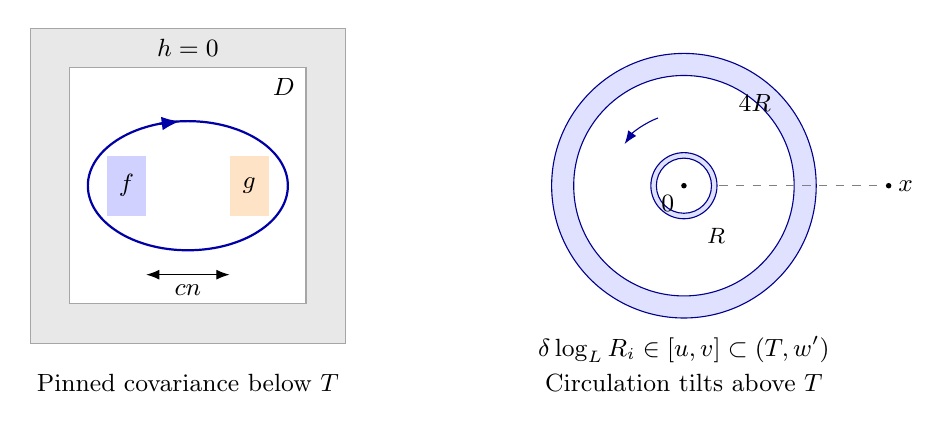
\begin{tikzpicture}[>=Latex,font=\small]
\begin{scope}[xshift=2.3cm,yshift=2.3cm]
 \fill[gray!18] (-2,-2) rectangle (2,2);
 \fill[white] (-1.5,-1.5) rectangle (1.5,1.5);
 \draw[gray!70] (-2,-2) rectangle (2,2);
 \draw[gray!70] (-1.5,-1.5) rectangle (1.5,1.5);
 \node at (0,1.75) {$h=0$};
 \node[anchor=north east] at (1.48,1.48) {$D$};
 \fill[blue!18] (-1.03,-.38) rectangle (-.53,.38);
 \fill[orange!22] (.53,-.38) rectangle (1.03,.38);
 \node at (-.78,0) {$f$};
 \node at (.78,0) {$g$};
 \draw[blue!65!black,thick] (0,0) ellipse[x radius=1.27cm,y radius=.82cm];
 \draw[->,blue!65!black,thick] (-.36,.786)--(-.1,.818);
 \draw[<->] (-.53,-1.13)--(.53,-1.13) node[midway,below] {$c n$};
 \node[align=center] at (0,-2.5) {Pinned covariance below $T$};
\end{scope}
\begin{scope}[xshift=8.6cm,yshift=2.3cm]
 \fill[blue!12,even odd rule] (0,0) circle (1.68) (0,0) circle (1.4);
 \fill[blue!12,even odd rule] (0,0) circle (.42) (0,0) circle (.35);
 \draw[blue!55!black] (0,0) circle (1.4);
 \draw[blue!55!black] (0,0) circle (1.68);
 \draw[blue!55!black] (0,0) circle (.35);
 \draw[blue!55!black] (0,0) circle (.42);
 \fill (0,0) circle (.035) node[below left] {$0$};
 \fill (2.6,0) circle (.035) node[right] {$x$};
 \draw[dashed,gray] (.45,0)--(2.53,0);
 \node at (.9,1.05) {$4R$};
 \node[below right,font=\footnotesize] at (.17,-.42) {$R$};
 \draw[->,blue!60!black] (-.33,.86) arc[start angle=111,end angle=145,radius=.92];
 \node[align=center] at (0,-2.08) {$\delta\log_LR_i\in[u,v]\subset(T,w')$};
 \node[align=center] at (0,-2.5) {Circulation tilts above $T$};
\end{scope}
\end{tikzpicture}
\caption{Two finite geometries for the mass comparison. Left: a primary pin region of positive width surrounds $D$. A loop contributing to the covariance of two separated density smears must have diameter at least their separation. The displayed loop is schematic. Right: geometrically spaced annuli surround one spin insertion and remain inside the separation scale of the other. Only two annuli are drawn. Their logarithmic scales lie in an interval where the height coefficient vanishes, so a fixed circulation tilt has arbitrarily small fluctuation cost on each annulus.}
\label{fig:mass-geometry}
\end{figure}


Choose a nonnegative, nonzero smooth radial function \(\chi\)
supported in \((1,2)\), and let
\[
       p(z)=\chi(|z|)\nabla\arg z,
       \qquad
       D=\int_{\R^2}p(z)\cdot\nabla\arg z\,dz>0.
\]
This is a smooth divergence-free form, compactly supported in the
unit annulus.  Choose its radial stream function \(\psi\), constant
on each complementary component, with \(\nabla^\perp\psi=p\).
At scale \(R\), sample \(\psi_R(z)=\psi(z/R)\) on the faces of
the primary height graph and take its rotated discrete difference.
Denote the resulting edge form by \(\eta_R\), choosing its sign
to agree with the positive source.  Thus, on an edge with midpoint
\(z_e\), its corresponding coordinate is
\(R^{-1}p(z_e/R)+O(R^{-2})\).
It has zero discrete divergence,
\begin{equation}\label{eq:mass-annulus-form}
 \max_e|\eta_R(e)|\le C/R,\qquad
 \sum_e|\eta_R(e)|^2\le C.
\end{equation}
For any affine height difference \(\nabla h+\alpha\) representing
the unit spin twist at \(0,x\), discrete summation by parts gives
\begin{equation}\label{eq:mass-deterministic-circulation}
 \sum_e\eta_R(e)(\nabla h+\alpha)_e=D_R,
                       \qquad D_R\longrightarrow D>0.
\end{equation}
Indeed the gradient part pairs to zero.  The remaining pairing is
the difference of the stream-function values at the two source
faces, multiplied by their circulations \(\pm2\pi\).
The stream function is constant near each source, so there is no
dependence on the height configuration or on the path chosen for
\(\alpha\).  The convergence in
\eqref{eq:mass-deterministic-circulation} also follows directly by
Riemann sums; its error is uniform here because the second source
lies outside every annulus.  Fix \(d_{\rm circ}>0\) so that \(D_R\ge d_{\rm circ}\)
for all sufficiently large radii.

We make the partition-ratio estimate at fixed \(k,x\) in a finite
free spin box large enough to contain all these annuli in its
interior.  Write \(Z_\alpha\) and \(Z_0\) for the twisted and
centered height sums, both with exterior face height zero.
Free-boundary duality gives \(C_{G,b_k}(0,x)=Z_\alpha/Z_0\).
For any fixed \(\lambda>0\), insertion of the deterministic tilt
from \eqref{eq:mass-deterministic-circulation} gives the exact identity
\begin{equation}\label{eq:mass-tilted-ratio}
 e^{\lambda\sum_{R\in\mathcal R_k}D_R}C_{G,b_k}(0,x)
 =\frac{Z_\alpha\left(
       e^{\lambda\sum_R(\eta_R,\nabla h+\alpha)}\right)}{Z_0}.
\end{equation}
Here \(Z_\alpha(F)\) means the unnormalized twisted sum with
insertion \(F\).  We will bound the right side independently of
the outer spin box.

Fix a small relative cell size \(t>0\).  Cover the support of each
\(\eta_R\) by square primary cells of side
\(m_R=\lfloor tR\rfloor\), with disjoint vertex sets, leaving
individual edges between cells as seam increments.  The support
of \(\chi\) has positive distance from the annular boundary.
Thus for sufficiently small fixed \(t\), every cell meeting this
support lies inside the annulus, avoids both sources, and is
simply connected.  There are \(O(t^{-2})\) such cells at each
radius.  Edges not in a retained cell and carrying a nonzero tilt
number \(O_t(R)\).

Release the endpoint constraints between these cells and the seam
increments, and release all remaining constraints outside the
cells.  The tilted affine-to-centered comparison
\cite[Lemma~2.2(ii)]{X} bounds the normalized expression in
\eqref{eq:mass-tilted-ratio} by the product of the cell transforms
and the independent whole-edge seam transforms.  Untilted factors
on the rest of the graph have affine-to-centered ratio at most
one.  On a retained cell the connection is an integral gradient,
\(\alpha=\nabla\kappa\); reindexing \(h'=h+\kappa\) removes it
from both the weight and the statistic being tilted.  Accordingly
the factor for that cell is the centered free transform
\[
             \E_{Q,b_k}^{\rm free}
                     \exp\{\lambda(\eta_R,\nabla h)_Q\}.
\]
In particular, this gauge change introduces no additional real
exponential factor.  Released constant modes are taken modulo
common translations; the edge-difference tests annihilate every
such constant.  Equivalently, one can retain vanishing quadratic
penalties on these constants in both sectors and cancel their
identical factors before removing them.  No outer-box normalizer
is present in the resulting bound.

We now estimate the factors for one annulus.  The total squared
coefficient cost of its seam increments is \(O_t(R^{-1})\) by
\eqref{eq:mass-annulus-form}.  The Bessel increment transform is
\(\exp\{b_k(\cosh(2\pi s)-1)\}\), so their combined logarithmic
cost is \(O_{t,\lambda}(R^{-1})\), uniformly in \(k\).
On each retained square replace \(\eta_R\) by its value at a
chosen point of the square.  Smoothness of \(p\) makes the total
squared cost of the coefficient error over all cells
\(O(t^2)+o_R(1)\).  The bounded-flow estimate \eqref{eq:bounded-flow-mgf} and
H\"older's inequality with exponent two therefore give
\begin{align}
 &\sum_Q\log\E_{Q,b_k}^{\rm free}
                  e^{\lambda(\eta_R,\nabla h)_Q}
 \notag\\[-2pt]
 &\qquad\le
 \frac12\sum_Q\log\E_{Q,b_k}^{\rm free}
                    e^{2\lambda(\bar\eta_{R,Q},\nabla h)_Q}
                       +C_\lambda t^2+o_{t,\lambda,R}(1),
 \label{eq:mass-affine-cell-reduction}
\end{align}
where \(\bar\eta_{R,Q}\) is the constant coefficient on \(Q\).
The error coefficients multiplied by the fixed tilt are uniformly
bounded, as required by \eqref{eq:bounded-flow-mgf}.  That estimate
bounds each error transform by its squared coefficient cost.
Summing the costs gives the total \(C_\lambda t^2\) in
\eqref{eq:mass-affine-cell-reduction}.

Each constant test in the sum is a linear combination of the two
square affine observations defining \(a_{m_R}(b_k)\).  Its
coefficient vector has size at most \(C_\lambda m_R/R\le C_\lambda t\).
Translations of the square do not change its law.  Moreover,
\[
       \delta_k\log_Lm_R
            =\delta_k\log_LR+\delta_k\log_Lt+o(1).
\]
Thus these scales lie in a slightly enlarged compact subinterval
of \((T,w')\) for all large \(k\).  By
Corollary~\ref{cor:profile-zero-uniform}, the transforms of these
affine tests tend uniformly to one, uniformly also in their
bounded coefficient vectors.  Since the number of cells is uniformly bounded
once \(t\) is fixed, their total logarithmic cost is \(o_k(1)\)
uniformly over \(R\in\mathcal R_k\).
The reference estimates and \(\min\mathcal R_k\to\infty\) also
make all seam and discretization errors uniform.  We obtain,
for every fixed \(\lambda,t\), the per-annulus bound
\begin{equation}\label{eq:mass-annulus-cost}
           \log(\text{product of its transforms})
                             \le C_\lambda t^2+o_k(1).
\end{equation}

Choose \(\lambda\) first, and then \(t\) so small that
\(C_\lambda t^2\le\lambda d_{\rm circ}/4\).  For all sufficiently large
\(k\), the uniform error in \eqref{eq:mass-annulus-cost} is at most
\(\lambda d_{\rm circ}/4\).  Equations~\eqref{eq:mass-tilted-ratio} and
\eqref{eq:mass-annulus-count} imply
\[
                    C_{G,b_k}(0,x)
                         \le\exp\{-\lambda d_{\rm circ}N_k/2\}.
\]
This estimate holds uniformly in every sufficiently large outer
spin box, at the fixed values of \(b_k,r_k,x\).  We may therefore
first take the prescribed free-box thermodynamic limit.  The
resulting estimate for \(C_{b_k}(x)\) is uniform in the indicated
range of \(x\).  Finally choose the fixed \(\lambda\) large enough
that \(\lambda d_{\rm circ}q/4>K\).  Equation~\eqref{eq:mass-annulus-count}
then gives \eqref{eq:mass-polynomial}.
\end{proof}

\subsection{A finite-size criterion and completion of the proof}

The Lieb--Rivasseau inequality for plane rotators
\cite{Lieb,Rivasseau}, in the form stated in
\cite[Lemma~17]{vEL}, says that for a finite subgraph \(H\subset G\),
\(u\in H\), and \(v\notin H\),
\begin{equation}\label{eq:mass-lieb-rivasseau}
 C_{G,b}(u,v)\le\sum_{z\in\partial H}
                       C_{H,b}(u,z)C_{G,b}(z,v).
\end{equation}
Here \(\partial H\) is the set of vertices of \(H\) adjacent to a
vertex outside \(H\); the first factor is the correlation with
free boundary on \(H\).  We give the iteration so its conclusion
refers to exactly the axis mass of this paper.

\begin{lemma}\label{lem:mass-finite-size}
Let \(H_r=[-r,r]^2\cap\Z^2\), and put
\[
                 S_{r,b}=\sum_{z\in\partial H_r}C_{H_r,b}(0,z).
\]
If \(S_{r,b}\le1/2\), then \(m(b)\ge(\log2)/r\).
\end{lemma}

\begin{proof}
At fixed \(b,r\), take the free-box thermodynamic limit in
\eqref{eq:mass-lieb-rivasseau}.  For a target \(se_1\), apply the
inequality successively in translates of \(H_r\) centered at the
boundary point reached in the previous step.  Each step moves the
center by at most \(r\) in the supremum norm.  Hence at least
\(\lfloor s/r\rfloor-1\) iterations are possible before the target
can belong to the next translated square.  Translation invariance
and \(C_b\le1\) give
\[
                   C_b(se_1)\le
                    S_{r,b}^{\lfloor s/r\rfloor-1}.
\]
Taking \(-s^{-1}\log\) and then \(s\to\infty\) proves the claim.
\end{proof}

\begin{proposition}\label{prop:mass-upper-length}
Along the extracted sequence,
\begin{equation}\label{eq:mass-limsup}
                 \limsup_k\delta_k\log_L\frac1{m(b_k)}\le T.
\end{equation}
\end{proposition}

\begin{proof}
Fix \(w'>T\), and set \(r_k=\lfloor L^{w'/\delta_k}\rfloor\).
Proposition~\ref{prop:mass-polynomial}, with any fixed \(K>1\),
and finite-to-infinite monotonicity imply
\[
 S_{r_k,b_k}\le\sum_{z\in\partial H_{r_k}}C_{b_k}(z)
                     \le8r_k\,r_k^{-K}<\frac12
\]
for all sufficiently large \(k\).  Thus
Lemma~\ref{lem:mass-finite-size} yields
\(m(b_k)\ge(\log2)/r_k\).  Consequently
\[
 \limsup_k\delta_k\log_L\frac1{m(b_k)}
 \le\lim_k\delta_k\log_L\frac{r_k}{\log2}=w'.
\]
Letting \(w'\downarrow T\) proves \eqref{eq:mass-limsup}.
\end{proof}

\begin{proof}[Proof of Theorem~\ref{thm:main}]
Start with any sequence \(b_k<b_c\) tending to \(b_c\).
The construction in Sections~\ref{sec:trajectory} and
\ref{sec:profile} admits a subsequence with the profile
\eqref{eq:mass-profile}.  Its transition point is
\[
                       T=\frac{\pi}{\sqrt{3\mathcal P}},
\]
where \(\mathcal P\in(0,\infty)\) is independent of the extracted
sequence.  Propositions~\ref{prop:mass-lower-length} and
\ref{prop:mass-upper-length} prove
\eqref{eq:mass-scale-goal} on that subsequence.
If the asserted limit failed for the original parameter approach,
there would be a sequence on which its distance from \(T\) stayed
bounded below; applying the same extraction to that sequence
would give a contradiction.  Therefore the logarithmic-scale
limit holds as \(b\uparrow b_c\) without extraction.
Converting from base \(L\) to natural logarithms gives
\[
 \lim_{b\uparrow b_c}\sqrt{b_c-b}\log\frac1{m(b)}
       =(\log L)\,T
       =\frac{\pi\log L}{\sqrt{3\mathcal P}}
       =:A_{\rm XY}\in(0,\infty).
\]
All spin correlations used above are limits of the prescribed
free spin boxes before their separation tends to infinity.  Thus
the mass in this identity is exactly the mass in
Theorem~\ref{thm:main}.
\end{proof}

\begin{thebibliography}{99}
\raggedright

\bibitem{AHPS}
M.~Aizenman, M.~Harel, R.~Peled, and J.~Shapiro,
Depinning in integer-restricted Gaussian fields and BKT phases of
two-component spin models,
preprint, revised May 27, 2022.
\href{https://arxiv.org/abs/2110.09498v3}{arXiv:2110.09498v3}.

\bibitem{BPR1}
R.~Bauerschmidt, J.~Park, and P.-F.~Rodriguez,
The Discrete Gaussian model, I. Renormalisation group flow at high temperature,
\emph{The Annals of Probability} \textbf{52} (2024), 1253--1359.
\href{https://doi.org/10.1214/23-AOP1658}{doi:10.1214/23-AOP1658}.

\bibitem{BPR2}
R.~Bauerschmidt, J.~Park, and P.-F.~Rodriguez,
The Discrete Gaussian model, II. Infinite-volume scaling limit at high temperature,
\emph{The Annals of Probability} \textbf{52} (2024), 1360--1398.
\href{https://doi.org/10.1214/23-AOP1659}{doi:10.1214/23-AOP1659}.

\bibitem{Berezinskii}
V.~L.~Berezinskii,
Destruction of long-range order in one-dimensional and two-dimensional
systems having a continuous symmetry group. I. Classical systems,
\emph{Soviet Physics JETP} \textbf{32} (1971), 493--500.
\href{https://www.jetp.ras.ru/cgi-bin/dn/e_032_03_0493.pdf}{English translation}.

\bibitem{DurandLammers}
T.~Durand and P.~Lammers,
The BKT transition and surface tension differentiability,
preprint, May 27, 2026.
\href{https://arxiv.org/abs/2605.28473v1}{arXiv:2605.28473v1}.

\bibitem{Falco}
P.~Falco,
Critical exponents of the two dimensional Coulomb gas at the
Berezinskii--Kosterlitz--Thouless transition,
preprint, revised November 25, 2013.
\href{https://arxiv.org/abs/1311.2237v2}{arXiv:1311.2237v2}.

\bibitem{FS}
J.~Fr\"ohlich and T.~Spencer,
The Kosterlitz--Thouless transition in two-dimensional Abelian spin systems
and the Coulomb gas,
\emph{Communications in Mathematical Physics} \textbf{81} (1981), 527--602.
\href{https://doi.org/10.1007/BF01208273}{doi:10.1007/BF01208273}.

\bibitem{Ginibre}
J.~Ginibre,
General formulation of Griffiths' inequalities,
\emph{Communications in Mathematical Physics} \textbf{16} (1970), 310--328.
\href{https://doi.org/10.1007/BF01646537}{doi:10.1007/BF01646537}.

\bibitem{Kosterlitz}
J.~M.~Kosterlitz,
The critical properties of the two-dimensional XY model,
\emph{Journal of Physics C: Solid State Physics} \textbf{7} (1974), 1046--1060.
\href{https://doi.org/10.1088/0022-3719/7/6/005}{doi:10.1088/0022-3719/7/6/005}.

\bibitem{KT}
J.~M.~Kosterlitz and D.~J.~Thouless,
Ordering, metastability and phase transitions in two-dimensional systems,
\emph{Journal of Physics C: Solid State Physics} \textbf{6} (1973), 1181--1203.
\href{https://doi.org/10.1088/0022-3719/6/7/010}{doi:10.1088/0022-3719/6/7/010}.

\bibitem{Lammers}
P.~Lammers,
Bijecting the BKT transition,
preprint, revised April 18, 2023.
\href{https://arxiv.org/abs/2301.06905v2}{arXiv:2301.06905v2}.

\bibitem{Lieb}
E.~H.~Lieb,
A refinement of Simon's correlation inequality,
\emph{Communications in Mathematical Physics} \textbf{77} (1980), 127--135.
\href{https://doi.org/10.1007/BF01982712}{doi:10.1007/BF01982712}.

\bibitem{Lupu}
T.~Lupu,
From loop clusters and random interlacements to the free field,
\emph{The Annals of Probability} \textbf{44} (2016), 2117--2146.
\href{https://doi.org/10.1214/15-AOP1019}{doi:10.1214/15-AOP1019}.
Author's version:
\href{https://arxiv.org/abs/1402.0298v7}{arXiv:1402.0298v7}.

\bibitem{X}
OpenAI,
The critical correlation exponent of the planar XY model,
OpenAI Math Release preprint
\href{https://github.com/openai/math/blob/main/preprints/The-critical-correlation-exponent-of-the-planar-XY-model-September-24-2026/paper.pdf}{OAI:The-critical-correlation-exponent-of-the-planar-XY-model-September-24-2026},
2026.

\bibitem{F}
OpenAI,
The critical logarithmic correction for the planar XY model,
OpenAI Math Release preprint
\href{https://github.com/openai/math/blob/main/preprints/The-critical-logarithmic-correction-for-the-planar-XY-model-October-5-2026/paper.pdf}{OAI:The-critical-logarithmic-correction-for-the-planar-XY-model-October-5-2026},
2026.

\bibitem{RSD}
O.~Regev and N.~Stephens-Davidowitz,
An inequality for Gaussians on lattices,
\emph{SIAM Journal on Discrete Mathematics} \textbf{31} (2017), 749--757.
\href{https://doi.org/10.1137/15M1052226}{doi:10.1137/15M1052226}.

\bibitem{Rivasseau}
V.~Rivasseau,
Lieb's correlation inequality for plane rotors,
\emph{Communications in Mathematical Physics} \textbf{77} (1980), 145--147.
\href{https://doi.org/10.1007/BF01982714}{doi:10.1007/BF01982714}.

\bibitem{vEL}
D.~van Engelenburg and M.~Lis,
An elementary proof of phase transition in the planar XY model,
\emph{Communications in Mathematical Physics} \textbf{399} (2023), 85--104.
\href{https://doi.org/10.1007/s00220-022-04550-3}{doi:10.1007/s00220-022-04550-3}.

\end{thebibliography}

\end{document}
